% This must be in the first 5 lines to tell arXiv to use pdfLaTeX, which is strongly recommended.
\pdfoutput=1
% In particular, the hyperref package requires pdfLaTeX in order to break URLs across lines.

\documentclass[11pt]{article}

% Change "review" to "final" to generate the final (sometimes called camera-ready) version.
% Change to "preprint" to generate a non-anonymous version with page numbers.
\usepackage[preprint]{acl}

% Standard package includes
\usepackage{times}
\usepackage{latexsym}

% For proper rendering and hyphenation of words containing Latin characters (including in bib files)
\usepackage[T1]{fontenc}
% For Vietnamese characters
% \usepackage[T5]{fontenc}
% See https://www.latex-project.org/help/documentation/encguide.pdf for other character sets

% This assumes your files are encoded as UTF8
\usepackage[utf8]{inputenc}

% This is not strictly necessary, and may be commented out,
% but it will improve the layout of the manuscript,
% and will typically save some space.
\usepackage{microtype}

% This is also not strictly necessary, and may be commented out.
% However, it will improve the aesthetics of text in
% the typewriter font.
\usepackage{inconsolata}

%Including images in your LaTeX document requires adding
%additional package(s)
\usepackage{graphicx}

\usepackage{amsmath}
\usepackage{booktabs}
\usepackage{amsfonts}
\usepackage{enumerate}
\usepackage{lipsum}
\usepackage{enumitem}
\usepackage{multirow}
\usepackage{pifont}
\usepackage{hyperref}

\newcommand{\zxy}[1]{{\color{blue} [#1 – Xy]}}
\newcommand{\zc}[0]{{\color{blue} [cite]}\xspace}
 % for Prof. Zhao
\newcommand{\w}[1]{{\color{orange}[#1]}} % Yejing
\newcommand{\fzc}[1]{{\color{red} #1}} % Zichuan
\newcommand{\swt}[1]{{\color{green} #1}} % Wentao


% \usepackage{xcolor}
% \pagecolor[rgb]{0,0,0} %black
% \color[rgb]{0.7,0.7,0.7} %grey

% If the title and author information does not fit in the area allocated, uncomment the following
%
%\setlength\titlebox{<dim>}
%
% and set <dim> to something 5cm or larger.

\title{Sliding Window Attention Training for Efficient Large Language Models}
% Long-Context Handling

% Author information can be set in various styles:
% For several authors from the same institution:
% \author{Author 1 \and ... \and Author n \\
%         Address line \\ ... \\ Address line}
% if the names do not fit well on one line use
%         Author 1 \\ {\bf Author 2} \\ ... \\ {\bf Author n} \\
% For authors from different institutions:
% \author{Author 1 \\ Address line \\  ... \\ Address line
%         \And  ... \And
%         Author n \\ Address line \\ ... \\ Address line}
% To start a separate ``row'' of authors use \AND, as in
% \author{Author 1 \\ Address line \\  ... \\ Address line
%         \AND
%         Author 2 \\ Address line \\ ... \\ Address line \And
%         Author 3 \\ Address line \\ ... \\ Address line}

% \author{First Author \\
%   Affiliation / Address line 1 \\
%   Affiliation / Address line 2 \\
%   Affiliation / Address line 3 \\
%   \texttt{email@domain} \\\And
%   Second Author \\
%   Affiliation / Address line 1 \\
%   Affiliation / Address line 2 \\
%   Affiliation / Address line 3 \\
%   \texttt{email@domain} \\}

% \author{
%  \textbf{Zichuan Fu\textsuperscript{1}},
%  \textbf{Wentao Song\textsuperscript{2}},
%  \textbf{Yejing Wang\textsuperscript{1}},
%  \textbf{Xian Wu\textsuperscript{3,†}},
% \\
%  \textbf{Yefeng Zheng\textsuperscript{3,4}},
%  \textbf{Yingying Zhang\textsuperscript{5}},
%  \textbf{Derong Xu\textsuperscript{1,6}},
%  \textbf{Xuetao Wei\textsuperscript{7}},
% \\
%  \textbf{Tong Xu\textsuperscript{6,†}},
%  \textbf{Xiangyu Zhao\textsuperscript{1,†}},
%  \textbf{Ziheng Zhang\textsuperscript{3}},
%  \textbf{Zhihong Zhu\textsuperscript{8}},
% \\
%  \textbf{Zhenxi Lin\textsuperscript{3}},
%  \textbf{Qidong Liu\textsuperscript{1,2}},
%  \textbf{Wanyu Wang\textsuperscript{1}},
%  \textbf{Yuyang Ye\textsuperscript{1}},
%  \textbf{Enhong Chen\textsuperscript{6}}
% \\
%  \textsuperscript{1}City University of Hong Kong, Hong Kong, China,
%  \textsuperscript{2}Xi'an Jiaotong University, Xi'an, China,
% \\
%  \textsuperscript{3}Jarvis Research Center, Tencent YouTu Lab, Shenzhen, China,
% \\
%  \textsuperscript{4}Medical Artificial Intelligence Lab, Westlake University, Shenzhen, China,
% \\
%  \textsuperscript{5}Tencent, Shenzhen, China,
%  \textsuperscript{6}University of Science and Technology of China, Hefei, China,
% \\
%  \textsuperscript{7}Southern University of Science and Technology, Shenzhen, China,
%  \textsuperscript{8}Peking University, Beijing, China
% \\
%  \small{
%    \textbf{Correspondence:} \href{mailto:xy.zhao@cityu.edu.hk}{xy.zhao@cityu.edu.hk}
%  }
% }

% \author{
%  Zichuan Fu\textsuperscript{1}, Wentao Song\textsuperscript{2}, Yejing Wang\textsuperscript{1}, Xian Wu\textsuperscript{3,†},
%  Yefeng Zheng\textsuperscript{3,4}, Yingying Zhang\textsuperscript{5}, 
%  Derong Xu\textsuperscript{1,6}, Xuetao Wei\textsuperscript{7},
%  Tong Xu\textsuperscript{6,†}, Xiangyu Zhao\textsuperscript{1,†}, Ziheng Zhang\textsuperscript{3}, Zhihong Zhu\textsuperscript{8},
%  Zhenxi Lin\textsuperscript{3}, Qidong Liu\textsuperscript{1,2}, Wanyu Wang\textsuperscript{1}, Yuyang Ye\textsuperscript{1},
%  Enhong Chen\textsuperscript{6}
% \\
% \\
%  \textsuperscript{1}City University of Hong Kong, Hong Kong, China, \textsuperscript{2}Xi'an Jiaotong University, Xi'an, China,
%  \textsuperscript{3}Jarvis Research Center, Tencent YouTu Lab, Shenzhen, China, \textsuperscript{4}Medical Artificial Intelligence Lab, Westlake University, Shenzhen, China,
%  \textsuperscript{5}Tencent, Shenzhen, China, \textsuperscript{6}University of Science and Technology of China, Hefei, China,
%  \textsuperscript{7}Southern University of Science and Technology, Shenzhen, China, \textsuperscript{8}Peking University, Beijing, China
% \\
%  Correspondence: xy.zhao@cityu.edu.hk
% }

\author{
  \textbf{Zichuan Fu\textsuperscript{1,\thanks{Work was conducted during the internship of Zichuan Fu at Tencent YouTu Lab.}}},
  \textbf{Wentao Song\textsuperscript{2}},
  \textbf{Yejing Wang\textsuperscript{1}},
  \textbf{Xian Wu\textsuperscript{3}},
  \textbf{Yefeng Zheng\textsuperscript{3,4}},\\
  \textbf{Yingying Zhang\textsuperscript{3}},
  \textbf{Derong Xu\textsuperscript{1,5}},
  \textbf{Xuetao Wei\textsuperscript{6}},
  \textbf{Tong Xu\textsuperscript{5}},
  \textbf{Xiangyu Zhao\textsuperscript{1,\thanks{Corresponding author.}}},
\\
\\
  \textsuperscript{1} City University of Hong Kong
  \textsuperscript{2} Xi'an Jiaotong University \\
  \textsuperscript{3} Jarvis Research Center, Tencent YouTu Lab 
  \textsuperscript{4} Westlake University \\
  \textsuperscript{5} University of Science and Technology of China \\
  \textsuperscript{6} Southern University of Science and Technology
\\
  \small{
   \href{mailto:zc.fu@my.cityu.edu.hk}{zc.fu@my.cityu.edu.hk},
   \href{mailto:xy.zhao@cityu.edu.hk}{xy.zhao@cityu.edu.hk}
  }
}



%\author{
%  \textbf{First Author\textsuperscript{1}},
%  \textbf{Second Author\textsuperscript{1,2}},
%  \textbf{Third T. Author\textsuperscript{1}},
%  \textbf{Fourth Author\textsuperscript{1}},
%\\
%  \textbf{Fifth Author\textsuperscript{1,2}},
%  \textbf{Sixth Author\textsuperscript{1}},
%  \textbf{Seventh Author\textsuperscript{1}},
%  \textbf{Eighth Author \textsuperscript{1,2,3,4}},
%\\
%  \textbf{Ninth Author\textsuperscript{1}},
%  \textbf{Tenth Author\textsuperscript{1}},
%  \textbf{Eleventh E. Author\textsuperscript{1,2,3,4,5}},
%  \textbf{Twelfth Author\textsuperscript{1}},
%\\
%  \textbf{Thirteenth Author\textsuperscript{3}},
%  \textbf{Fourteenth F. Author\textsuperscript{2,4}},
%  \textbf{Fifteenth Author\textsuperscript{1}},
%  \textbf{Sixteenth Author\textsuperscript{1}},
%\\
%  \textbf{Seventeenth S. Author\textsuperscript{4,5}},
%  \textbf{Eighteenth Author\textsuperscript{3,4}},
%  \textbf{Nineteenth N. Author\textsuperscript{2,5}},
%  \textbf{Twentieth Author\textsuperscript{1}}
%\\
%\\
%  \textsuperscript{1}Affiliation 1,
%  \textsuperscript{2}Affiliation 2,
%  \textsuperscript{3}Affiliation 3,
%  \textsuperscript{4}Affiliation 4,
%  \textsuperscript{5}Affiliation 5
%\\
%  \small{
%    \textbf{Correspondence:} \href{mailto:email@domain}{email@domain}
%  }
%}

\begin{document}


\maketitle
\begin{abstract}
Recent advances in transformer-based Large Language Models (LLMs) have demonstrated remarkable capabilities across various tasks. However, their quadratic computational complexity concerning sequence length remains a significant bottleneck for processing long documents. As a result, many efforts like sparse attention and state space models have been proposed to improve the efficiency of LLMs over long sequences. 
While these approaches achieve efficiency, they often require complex architectures and parallel training techniques.
This calls for a simple yet efficient model that preserves the fundamental Transformer architecture. 
To this end, we introduce \textbf{SWAT}, which enables efficient long-context handling via \textbf{S}liding \textbf{W}indow \textbf{A}ttention \textbf{T}raining. 
Specifically, SWAT replaces softmax with the sigmoid function for efficient information compression and retention. Then it utilizes balanced ALiBi and Rotary Position Embedding to stabilize training process. 
During inference, SWAT maintains linear computational complexity through sliding window attention while preserving model performance, achieving state-of-the-art (SOTA) results on eight commonsense reasoning benchmarks compared to mainstream linear recurrent architectures.
Code is available at \href{https://anonymous.4open.science/r/SWAT-attention}{this link}.

% and utilize a balanced ALiBi and Rotary Position Embedding
% This paper first attributes the inefficiency of Transformers to the attention sink phenomenon resulting from the high variance of softmax operation. Then, we replace softmax with the sigmoid function and utilize a balanced ALiBi and Rotary Position Embedding for efficient information compression and retention. 
    %This motivates us to design a simple yet efficient model that preserves the fundamental transformer architecture.
    %This paper introduces \textbf{SWAT}, which enables efficient long-context handling via \textbf{S}liding \textbf{W}indow \textbf{A}ttention \textbf{T}raining. 
    % Through experimental analysis, we reveal that Transformers suffer from attention sink phenomenon due to the variance brought by softmax. 
   
    % To address these issues, we replace softmax with the sigmoid function and utilize a balanced ALiBi and Rotary Position Embedding for efficient information compression and retention.
    
    % Our approach enables efficient long-context processing without requiring complex architectural changes or inference-time adjustments, providing a practical solution for developing more efficient LLMs. 

\end{abstract}

Stochastic systems have been used extensively in several areas including  verification~\cite{FKNP11}, learning theory~\cite{AJKS21}, epidemic processes~\cite{Lef81} to name a few. Several real-world systems however do not work with a centralised control. Therefore, modelling using stochastic systems with multiple agents makes for more faithful abstractions of such systems without a centralised control. Some examples of fields in which multi-agents stochastic modelling include cyber physical systems~\cite{SEC16}, distributed and probabilistic computer programs~\cite{dAHJ01}, probabilistic planning~\cite{TKI10}. In such cases, the problem of reasoning about multiple agents with several, often times orthogonal objectives, becomes important. % However, for situations that are modelled as graph games, Nash equilibria come with its own down-sides and therefore several notions of equilibria have emerged in turn-based games on graphs to circumvent the problems posed by the natural definitions of Nash equilibira, like subgame-perfect equilibira, Stackleberg-equilibria. 
For multi-agent systems modelled with stochasticity on the underlying arena, a fundamental question to ask is the existence or finding of an equilibrium.
The most popular equilibria in literature are Nash equilibria~\cite{Nas50}. However, those come with their own downsides. The computational complexity for studying Nash equilibria over multi-agent systems is prohibitively expensive, and even undecidable in the general case, where systems have $10$ or more players~\cite{UW11}. 
Further, even if Nash equilibria could be computed efficiently, they do not faithfully model the agents in real world settings
%as each agent might perceive risk differently. With randomness arising from both the strategies of other agents, as well as the underlying model of the system, this might mean that risk-averse or risk-loving agents might have an incentive to deviate since their perceived values of outcome is different from expected value of the game.
since they do not consider their tolerance or averseness to risk.

Let us consider a $1$-player game where a protagonist is proposed two options: (a) earning \$1; (b) playing a lottery in which, with probability $\frac{1}{40}$, she gets \$40, and with probability $\frac{39}{40}$, she does not earn anything.
Classically, rational strategies would be maximising the expected payoff. From this perspective, both options yield an expected payoff of \$1, making them equivalent.
This approach is particularly justified when the game represents a scenario that can be repeated many times: the law of large numbers ensures that, in the long run, the average payoff will converge to the expected payoff. However, when the game is played only once, the protagonist may prioritise immediate needs. If she urgently requires \$1, the guaranteed option (a) becomes preferable.

Conversely, if she is a risk-taker or finds herself in a situation where only the \$40 can make a significant difference, she may prefer the high-risk option (b).
Although this choice might appear irrational, it mirrors the behaviour of millions of people who participate everyday in games with a negative expected payoff, driven by the allure of a potentially life-changing win, and generating an annual turnover of USD 536 billions~\cite{GamblingNewspaper23} for the gambling industry.
That industry, on the other hand, operates on a large scale where expected payoff becomes the key metric. 
This contrast underscores the importance of alternative measures to expected payoff that account for each agent's risk tolerance.%, offering a more nuanced understanding of decision-making in uncertain scenarios.

%We thus have an example of a two-player interaction, with apparently zero-sum payoffs, but where both players express a preference for the same option, because the context gives them a different tolerance to risk: this paradox underscores the importance of alternative measures to expected payoff that account for an agent's risk tolerance, offering a more nuanced understanding of decision-making in uncertain scenarios.
% This contrast underscores the relevance of generalising the notion of Nash equilibria: in a multi-agent system, the agents may have diverging perception of which risks can be taken.
% It makes sense, then, to study \emph{risk-sensitive equilibria}, in which players do not necessarily maximise their expected payoff, but their perception of what their payoff will be according to different risk measures.\leon{I'm actually not satisfied with this, I will modify it and move it.}


% Classically, we consider that a rational strategy would consist in maximising the expected payoff: from that perspective, the two choices are equivalent.
% Such an approach is justified especially when the game models a situation that can be repeated a large number of times, in which case the law of large numbers guarantees that the average payoff converges to the expected payoff.
% But when the game models a situation that is played only once, the protagonist may consider that she really needs her euro, and that the possibility of earning 40\$ is too unlikely to be taken into account: she would then have a justifiable preference for the option (a).
% On the contrary, if she is more of a gambler, or if she finds herself in a desperate situation in which only earning those 40\$ could save her, she could go all out and express a strict preference for option (b)\footnote{Even though this case seems more irrational, it explain why millions of people play everyday games in which they know that their expected payoff is negative.
% On the other side, the companies with whom they interact repeat the experience often enough to consider expected payoff as the relevant measure --- generating a yearly turnover of 536 billions of US\$.}.
% Hence the relevance of alternatives to expected payoff, that take into account the tolerance of the agent to risk.

\subparagraph*{Risk Measures.}
A \emph{risk measure} captures the perception that a player has of what their payoff will be. In that sense, they generalise the notion of expected payoff.
Various risk measures exist in the literature, and have been used extensively in the field of economics and finance. 
Some of these risk measures include expected shortfall (ES), value at risk (VaR)~\cite{Aue18}, variance~\cite{Bra99}, entropic risk measure (ER)~\cite{FS02}. 

%However, since the introduction of the characteristic of risk measure called \emph{coherence}~\cite{ADJH99}, it was expected that a ``good'' a risk measure must be coherent. A risk measure is coherent if it is monotonic, homogeneous, translational-invariance, and sub-additive.
%This automatically weeds out several of the above risk measures listed above like  Value at Risk or variance as a risk measure. 
A lot of work has been done in considering these risk measures over MDPs which use variance (along with mean) as a risk-measure~\cite{FK89, PSB22,MT11}, ES~\cite{RRS15,KM18,Meg22} (also referred to as conditional value at risk (CVaR), average value at risk (AVaR), expected tail loss (ETL), and superquantile in literature) and ER~\cite{HM72,BR14,BCMP24}. % have also been studied. 
Studying the entropic risk measure in MDPs appears more practical compared to expected shortfall  or using variance-penalised risk-measures. This impracticability of ES and variance-penalised measure in particular is due to the intractable exponential memory~\cite{HK15} and time required to compute optimal strategies~\cite{PSB22}, even for the one agent system of Markov decision processes (MDPs). On the other hand, when the risk measure used is ER, players have optimal positional strategies in MDPs~\cite{How72}, which makes it a prime candidate for consideration in multi-agent settings.

\subparagraph*{Entropic Risk Measure.}
The entropic risk measure is computed by assigning to each agent a risk parameter, i.e., a value $\rho \in \Rb$.
%Based on this risk parameter $\rho$, this measure first computes the expectation of the exponential function of the random variable and then re-normalises this.  
The entropic risk measure of a random variable $X$ is then defined as
$\re_\rho[X] = -\frac{1}{\rho} \log_e \left( \Eb \left[ e^{-\rho X}\right] \right)$. 
%For computational reasons, instead of the Euler's constant $e$, we use different bases sometimes.
If the risk parameter $\rho$ is positive, then more weight will be given to the bad payoffs: the corresponding player can then be considered as risk-averse.
Conversely, players with a negative $\rho$ are more risk-loving.
When $\rho$ tends to $0$, the entropic risk measure converges to the classical expectation $\Eb[X]$.

The game depicted by Figure~\ref{fig:example_gamma} extends the lottery example we discussed earlier. 
Black vertices are stochastic, and the circle vertex is controlled by player $\Circle$.
A play can be seen as an infinite sequence of moves of a token along the edges of the graph, starting from $a$: from a stochastic vertex, it takes one of the outgoing edges with the probabilities indicated on those, and from a vertex controlled by the player, she chooses which edge it takes.
The payoff $40$, $0$, or $1$ is obtained when the terminal vertex $t_1$, $t_2$, or $t_3$ is reached, respectively.
If no terminal vertex is reached, then the payoff is $0$.
Taking the red edge corresponds to option (a): then, her risk entropy is always $1$, for every risk parameter $\rho$.
But if she chooses option (b), that is, if she takes the blue edge, her risk entropy is $\re_\rho[\mu_{\circ}] = -\frac{1}{\rho} \log \left( \Eb \left[ e^{-\rho \mu_{\circ}}\right] \right) = -\frac{1}{\rho} \log \left(  e^{-40\rho } + \frac{39}{40} \right)$.
Both cases are illustrated with red and blue curves in \cref{fig:example_plot}.
The curves cross at abscissa $\rho = 0$, where the entropic risk measure corresponds to the expectation. Note that other strategies are possible if \emph{randomisation} is allowed---the player could, for example, toss a coin and participate in the lottery if the outcome is heads. The perceived reward of randomising between outermost red and blue edges are illustrated in the intermediate cases with mixtures of red and blue in \cref{fig:example_plot}.

%For this example, we  replace Euler's constant $e$ with instead the constant $2$, which makes $\re_\rho[X] = -\frac{1}{\rho} \log_2 \left( \Eb \left[ 2^{-\rho X}\right] \right)$.

%Player $\Circle$ gets the payoff $11$ if she reaches the terminal vertex $t_1$, the payoff $1$ if she reaches $t_2$, the payoff $2$ if she reaches $t_3$, and the payoff $0$ if she reaches none of those terminal states (i.e., if she loops on the vertex $a$ forever).

%If the player's strategy is to choose the red edge, she gets payoff $1$ with probability $1$.
%Therefore, her risk measure is equal to $1$ for every risk parameter $\rho$.

%If her strategy is to choose the blue edge going to $c$, then she gets the payoff $11$ with probability $\frac{1}{10}$, and $1$ with probability $\frac{9}{10}$.
%Thus her risk entropy is
%$\re_\rho[\mu_{\circ}] = \frac{1}{\rho} \log_2\left(\frac{1}{3} 2^{-4\rho} + \frac{2}{3} 2^{-1\rho}\right)$.
 
\begin{figure}[h] 
			\centering
            \begin{subfigure}[t]{0.4\textwidth}
			\begin{tikzpicture}[->,>=latex,shorten >=1pt, initial text={}, scale=1, every node/.style={scale=1}]
				\node[initial left, stoch] (a) at (0, 0) {$a$};
				\node[state] (b) at (1.5, 0) {$b$};
                \node[stoch] (c) at (2.5, 1) {$c$};
                \node (t1) at (4, 2) {$t_1:~\stack{\circ}{40}$};
                \node (t2) at (4, 0) {$t_2:~\stack{\circ}{0}$};
                \node (t3) at (3, -1) {$t_3:~\stack{\circ}{1}$};
                \path (a) edge[loop above] node[above] {$\frac{1}{2}$} (a);
				\path (a) edge node[above] {$\frac{1}{2}$} (b);
                \path (b) edge[blue, thick] (c);
                \path (b) edge[red, thick] (t3);
				\path (c) edge node[above] {$\frac{1}{40}$} (t1);
				\path (c) edge node[below] {$\frac{39}{40}$} (t2);
			\end{tikzpicture}
			\caption{A stochastic MDP}
			\label{fig:example_gamma}
            \end{subfigure}
            \begin{subfigure}[t]{0.55\textwidth}
			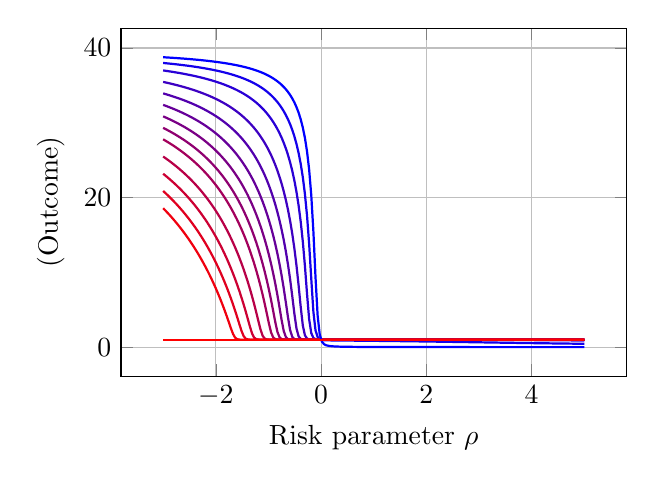
\begin{tikzpicture}
              \begin{axis}[
                xlabel={Risk parameter $\rho$},
                ylabel={$\re(\text{Outcome})$},
                domain=-3:5,
                samples=200,
                    width=8cm,
                   height=6cm,
                grid=major,
                ]
                \addplot [
                  red!8!blue,
                  thick
                ]
                {-1/x * log2((9/10)*e^(-1*x) + (1/400) * e^(-40*x) + (39/400))/log2(e)};
                \addplot [
                  red!16!blue,
                  thick
                ]
                {-1/x * log2((199/200)*e^(-1*x) + (1/8000) * e^(-40*x) + (39/8000))/log2(e)};
                \addplot [
                  red!24!blue,
                  thick
                ]
                {-1/x * log2((19999/20000)*e^(-1*x) + (1/800000) * e^(-40*x) + (39/800000))/log2(e)};
                \addplot [
                  red!32!blue,
                  thick
                ]
                {-1/x * log2((1999999/2000000)*e^(-1*x) + (1/80000000) * e^(-40*x) + (39/80000000))/log2(e)};
                \addplot [
                  red!40!blue,
                  thick
                ]
                {-1/x * log2((199999999/200000000)*e^(-1*x) + (1/8000000000) * e^(-40*x) + (39/8000000000))/log2(e)};
                \addplot [
                  red!48!blue,
                  thick
                ]
                {-1/x * log2((19999999999/20000000000)*e^(-1*x) + (1/800000000000) * e^(-40*x) + (39/800000000000))/log2(e)};
                \addplot [
                  red!56!blue,
                  thick
                ]
                {-1/x * log2((1999999999999/2000000000000)*e^(-1*x) + (1/80000000000000) * e^(-40*x) + (39/80000000000000))/log2(e)};
                \addplot [
                  red!64!blue,
                  thick
                ]
                {-1/x * log2((199999999999999/200000000000000)*e^(-1*x) + (1/8000000000000000) * e^(-40*x) + (39/8000000000000000))/log2(e)};
                \addplot [
                  red!72!blue,
                  thick
                ]
                {-1/x * log2((199999999999999999/200000000000000000)*e^(-1*x) + (1/8000000000000000000) * e^(-40*x) + (39/8000000000000000000))/log2(e)};
                \addplot [
                  red!80!blue,
                  thick
                ]
                {-1/x * log2((199999999999999999999/200000000000000000000)*e^(-1*x) + (1/8000000000000000000000) * e^(-40*x) + (39/8000000000000000000000))/log2(e)};
                \addplot [
                  red!88!blue,
                  thick
                ]
                {-1/x * log2((199999999999999999999999/200000000000000000000000)*e^(-1*x) + (1/8000000000000000000000000) * e^(-40*x) + (39/8000000000000000000000000))/log2(e)};
                \addplot [
                  red!94!blue,
                  thick
                ]
                {-1/x * log2((199999999999999999999999999/200000000000000000000000000)*e^(-1*x) + (1/8000000000000000000000000000) * e^(-40*x) + (39/8000000000000000000000000000))/log2(e)};
                \addplot [
                  blue,
                  thick
                ]
                {-1/x * log2((1/40) * e^(-40*x) + (39/40))/log2(e)};
                \addplot [
                  red,
                  thick
                ]
                {+1};
              \end{axis}
            \end{tikzpicture}
			\caption{Each curve represents the perceived reward of a player choosing only blue strategy, only red, or  randomising between both strategies. The percieved payoff for a player with risk parameter $\rho \in (-3,5)$ for these strategies are represented.}
			\label{fig:example_plot}
            \end{subfigure}
        \caption{Entropic risk measure}\label{fig:example_re}
\end{figure}
%\end{example}
Unfortunately, even for two player zero-sum stochastic games with total-reward objectives (payoff is the sum of the rewards seen along the way), computing optimal strategies can only be done in $\PSPACE$, when the base $e$ is replaced by an algebraic number; and if $e$ is the base of the exponent, then it is decidable only subject to Shanuel's conjecture~\cite{BCMP24}. % and inputs where the risk is computed using ER. 
Solving the two-player zero-sum case is a specific case of finding equilibria in two-agent systems where the payoffs of the two agents are exactly the negation of each others and so are the risk parameters of each of the agents.
Therefore, reasoning about multi-agent systems with ER also has potential to be computationally intractable.%\leon{I'm not sure I understand this sentence}


% \subparagraph*{Equilibria}
% Our example involves only one player.
% However, one might model it with a second player: the company that sells the lottery ticket, and therefore that made the choice of making the game possible.
% Of course, in the real world, companies only enable such games when its expected payoff is positive, that is, when the player's expected payoff is negative; which does not prevent millions of players to participate in such lotteries everyday, generating an annual turnover of USD 536 billion~\cite{h2_gambling_2023}.
% This can be explained by the fact that players are ready to take an important risk there, because they play a small number of times, and their likely loss remains acceptable, while their possible earning would be huge: in other words, players are efficiently modelled by a negative risk parameter.
% On the other hand, the company repeats the game a very large number of times, which is why, from its perspective, the expected payoff is the relevant metric.
% %This contrast underscores the importance of alternative measures to expected payoff that account for an agent's risk tolerance, offering a more nuanced understanding of decision-making in uncertain scenarios.
% This contrast underscores the relevance of generalising the notion of Nash equilibria: in a multi-agent system, the agents may have diverging perception of which risks can be taken.
% It makes sense, then, to study \emph{risk-sensitive equilibria}, in which players do not necessarily maximise their expected payoff, but their perception of what their payoff will be according to different risk measures.\leon{I'm actually not satisfied with this, I will modify it and move it.}



\subparagraph*{Extreme Risk Measure.} We introduce a new risk measure called extreme risk measure (XR) to identify tractable risk parameters. %\leon{Do we actually use that notation?} 
% If they have to choose between two options: (a) one which always gives him an outcome of 1, and the other option (b) that gives him a positive probability $p$ of 100, but  probability $(1-p)$ of -1, he would always chose option (a), 
%
%Let us say in a stochastic system, one agent is tasked with a safety-critical objective and wishes to avoid any positive probability of getting a payoff below some threshold, say $0$.
Consider an agent who wishes to maximise the lowest payoff received with positive probability.
In our example, 
by choosing option (a) her only payoff is $\$1$, whereas by choosing option (b), the payoffs that she receives with positive probability are $\$40$ and $\$0$. 
This agent would choose the option (a) since, then, the lowest reward she gets is $\$1$, instead of $\$0$. This would be her choice regardless of the probabilities or if the lottery amount in option (b) is increased.
%Even when the probabilities are changed for option (b) or if the lottery amount is increased, she would still prefer option (a).
Such agents can be considered ``extreme pessimists'' because
their perceived payoff can be thought of as the minimum among all the possible payoffs.
%We define the perceived reward of an extreme pessimist as the infimum of the payoffs that they get with positive probability. Therefore, extreme pessimists aim to maximise the smallest payoff that they receive with positive probability, and might be willing to deviate to achieve this objective.  
Similarly, one can define ``extreme optimists''  whose perceived reward is the best payoff that can be obtained with positive probability.
In the above scenario, an extreme optimist posed with the same options would choose option (b), no matter how small the probability is of receiving that payoff.

Extreme pessimists can be used to model safety-critical agents, where any positive probability of low reward or failure is unacceptable.
On the other hand, extreme optimists model naturally the opponents of such agents.
In a multiplayer setting, they can be an accurate modelling of agents like hackers in a system, who are happy with a small probability of success, or agents that have the possibility to restart their interactions with the same system, so that as long as there is a non-zero probability of achieving a high reward, they are guaranteed to receive that high reward. %\theju{If at all we discuss motivation here is the space.}





%\begin{example}
% Consider the same example game as in \cref{fig:example_gamma}. Here, the reward that the player perceives in the MDP can perceive on using the red strategy is exactly $2$ since that is the only payoff the player can get with a positive probability.
% However, if using the blue strategy, the perceived reward depends on if the player is an optimist or a pessimist. If the players is a pessimist, then the perceived reward is $4$, and if instead the player is an extreme pessimist, then the perceived reward is $1$.
%\end{example}
% \thejaswini{Introduce with examples some systems that need to be designed where some agent needs sure reward, and agents that some agents are happy with non-zero probability of reward}

%We capture this concept of extreme optimism and pessimism by introducing a new risk measure of pessimistic expectation and optimistic expectation.
\subparagraph*{Our results.}
We consider the problem of finding equilibria in a multiplayer stochastic game, that is, a game in which the payoffs that the players receive depend on the \emph{terminal vertex} that is reached, and in which an infinite play is associated to the zero payoff vector.

Our contributions are four fold. 
Firstly, we consider the problem of finding equilibria where entropic risk measure is used to determine the perceived reward of each player.  Each player has their own risk-sensitivity parameter, and we wish to find an equilibrium where no player has the incentive to deviate and increase their risk measure. We show that, when the rewards are all non-negative, such an equilibrium always exists.
We conjecture that this remains true when rewards can be negative.
Although some equilibria exist, not all equilibria are made the same, with some equilibria being more desirable than the others. One might want to find an equilibrium that maximises the overall social welfare, or want to minimise it for certain agents. A reasonably general setting is providing an interval for the risk measure for each agent and to check if there is an equilibrium satisfying these constraints. We call this problem \emph{constrained existence problem of risk-sensitive equilibria} (RSEs). 
We show (in \cref{sec:ERM}) that this problem is undecidable when the risk parameters of the players are rational values, with undecidability results extending from the constrained existence problem for Nash equilibria in the work of Ummels and Wojtczak~\cite{UW11}. However, we find restrictions on strategies to recover decidability. % for risk-sensitive equilibria in the cases where the risk parameters are finite.
If we restrict the memory requirements of each player, then for (small) finite memory strategies, we can solve the problem by encoding it using the existential theory of reals with exponentiation, giving us decidability subject to Shanuel's conjecture, and $\PSPACE$ algorithms when the base of the exponents are encoded as small algebraic instances, reminiscent of the two-player zero-sum case by Baier et al.~\cite{BCMP24}. 
%(\cref{proposition:Undecidable}).

Secondly, since the general problem is undecidable, and even in restricted cases, we obtain complexities that are $\PSPACE$ or higher, we pivot to searching for a more tractable risk measure that can be used to find equilibria in multi-agent systems. We define extreme risk measure (XR) as a novel risk measure to consider in multi-agent stochastic systems. We show (in \cref{sec:XR}) that our new definition is robust, since it exactly captures the well-studied entropic risk measure when the risk parameters tend to $\pm \infty$.
%This result (\cref{thm:RE=PEorOE}) in turn ensures that our risk measure is a robust definition since it is the limit of a well-studied risk measure. 
We further show the existence of 
such equilibria for games with non-negative rewards. Moreover, there exists a stationary strategy profile that can be algorithmically constructed in polynomial time. We conjecture, again, that this remains true when negative rewards are involved.
One further advantage of XR as a risk measure is that it is indifferent to the exact probabilities of the underlying stochastic model, since it only deals with events that occur with a positive probability and, therefore, can also be used in systems where the underlying probabilities are unknown. 

Thirdly, we show that the constrained existence problem of RSEs is decidable and also $\NP$-complete when the perceived payoff is calculated using XR, where each agent is either an extreme optimist or pessimist. The $\NP$ membership is nontrivial and follows several steps. First, we show that if there is a strategy that satisfies the constraints, then there is a finite abstraction of this strategy. Later, we show that this finite abstraction of the strategy has a polynomial representation. 
With this polynomial representation of the strategy, we show that verifying whether a given polynomially represented strategy is a risk-sensitive equilibrium that satisfies the constraints can also be done in polynomial time. 
Finally, we show that if all players are extreme optimists, this problem is $\PTIME$-complete.%, and provide a polynomial time algorithm for the constrained existence problem.
%\thejaswini{We add to this list by introducing a new risk measure that captures the above situation of extreme optimism and pessimism.}
%\thejaswini{We argue that our definition is robust, since this exactly captures the ERisk measure when the parameters are set to $-\infty$ and $+\infty$}
% \thejaswini{When the parameters are anywhere that are not $\pm\infty$, we show that computing Equilibria where ERisk is the outcome is undecidable. }
% \thejaswini{Argue that however, computational costs of precisely computing RSE for such values for stochastic games are undecidable}
% \thejaswini{This makes our definition the only decidable fragment for finding equilibria with entropic risk as a measure decidable}

\section{Understanding Transformer's Attention}


\begin{figure*}[ht]
    \hfill
    \includegraphics[width=\linewidth]{imgs/figure2.pdf}
    \caption{The $\log_{10}$ perplexity of four LLMs (Llama-2-7b, Llama-3.1-8B, Qwen2-7B and Mistral-7B-v0.1) on the third book of PG-19 test set using SWA inference. The window sizes are set not to exceed their respective training sequence lengths. The x-axis represents the sliding window size, and the y-axis represents the evaluation sequence length. For a fixed window size, perplexity increases (color shifts to blue) as the evaluation length grows.}
    \label{fig:open-llms}
\end{figure*}

\begin{figure*}[ht]
    \centering
    \includegraphics[width=\linewidth]{imgs/figure3.pdf}
    \caption{Heatmaps of attention scores (top four squares) and token embedding variance (bottom four lines) across different layers of Qwen2-7B. Higher token variance corresponds to stronger attention, highlighting their correlation. The two color bars indicate respective scales.}
    \label{fig:variance}
\end{figure*}

This section introduces concepts of the SWA mechanism and its potential capability in handling long sequences. We then analyze why current LLMs with SWA inference fail to achieve the expected theoretical advantages. 
% fail to perform SWA inference despite its theoretical advantages.

\subsection{Sliding Window Attention}

The self-attention layer in Transformers typically has $O(N^2)$ computational complexity, where $N$ is the input sequence length. 
To reduce this complexity while preserving the sequential information, sliding window attention (SWA) is introduced in Longformer~\cite{Longformer}. 
SWA restricts each token to only attend the attention calculation of its neighboring tokens within a fixed-size window.
% SWA restricts each token to attend only to its neighboring tokens within a fixed-size window.
With a window size of $\omega \ll N$, the computation cost per token is reduced to $O(\omega)$, leading to an overall linear complexity $O(N \cdot \omega)$, which is more efficient than vanilla attention.

We visualize the SWA mechanism in Figure~\ref{fig:swa}, where the window size is three ($\omega=3$) and the depth is two ($L=2$).
We define the tokens that are visible to the current window as active tokens (the red block in the figure, corresponding active tokens are ``a dear little'').
For invisible tokens, also referred to as evicted tokens, we further categorize them as residual and past tokens. 
Residual tokens are not visible to the sliding window at the embedding layer. However, their information will passed to the neighboring $\omega -1$ tokens with a transformer layer (this information transition is represented as yellow lines in the figure), thus partially preserved for the prediction. For example, the information of the token `a' (the orange ball at the embedding layer) can be retained in the other token `a' (the red ball at the second transformer layer) in our visualization. Theoretically, the information range of a single token at the $l^{th}$ transformer layer is $1+(\omega-1) \cdot l$ and the maximum range is $1+(\omega-1) \cdot L$, i.e., $1+2\cdot2=5$ in the figure.

% Among them, the information on the active tokens is fully accessible to the model since their embeddings are still within the attention window. For the latter two categories, referred to as evicted tokens, their embeddings have been discarded and are no longer visible to the model. However, residual tokens' information is preserved in the higher transformer layers, allowing the model to utilize this retained information during inference. With each additional transformer layer, the residual tokens retained in the higher layers expand by $(\omega-1)$ tokens. Therefore, the theoretical maximum range of information coverage in a SWA-based transformer is $(\omega-1) \cdot L + 1$, where $L$ denotes the number of transformer layers.

% Therefore, theoretically, evicted tokens (i.e., tokens whose key-value cache is discarded) are not indispensable for maintaining the model's performance as long as their information is effectively retained and propagated through the higher layers of the transformer. Empirically, larger window sizes, deeper models, and longer training sequences result in better performance.

\subsection{LLMs with SWA Inference}
%\subsection{Why current LLMs fail using SWA?}
\label{ssec:why}


Although current open-source LLMs are structurally capable of conducting SWA inference, they fail to achieve stable improved results. As shown in Figure~\ref{fig:open-llms}, we analyzed the perplexity (PPL) of four open-source LLMs~\cite{llama2,llama3,mistral-7b,qwen2} using different sliding window sizes on the PG-19~\cite{pg19} test set. The experimental results reveal that these LLMs achieve optimal performance only when operating within their training sequence length. For instance, for Llama-2-7b model in Figure~\ref{fig:open-llms}(a), when the window size is fixed at 1,024, the perplexity gradually increases as the evaluation length grows, as indicated by the color transition from blue to red in the heatmap.
This suggests that Transformers inherently learn contextual patterns specific to their training length and fail to extend to variable-length texts during inference.
% This limitation suggests that transformers inherently learn attention patterns specific to their training context length, making them poorly suited for processing variable-length texts during inference.

We suggest that this failure can be attributed to two major issues:
(1) the attention sink phenomenon, where models become overly dependent on initial tokens, 
and (2) information loss that past tokens are discarded.

The attention sink phenomenon~\cite{streamingllm}, where LLMs allocate excessive attention to initial tokens in sequences, has emerged as a significant challenge for SWA inference in Transformer architectures. Previous work has made two key observations regarding this phenomenon. First, the causal attention mechanism in Transformers is inherently non-permutation invariant, with positional information emerging implicitly through token embedding variance after softmax normalization~\cite{variance}. Second, studies have demonstrated that removing normalization from the attention mechanism can effectively eliminate the attention sink effect~\cite{whensinkemerge}.

% \textbf{Lemma 1:} The causal attention in Transformers is not permutation invariant inherently. The positional information emerges from the variance of token embeddings after the normalization operation of the softmax function~\cite{variance}.

% \textbf{Lemma 2:} \citet{whensinkemerge} demonstrates that removing normalization from attention eliminates the attention sink phenomenon~\cite{streamingllm}.

Based on these insights, we analyze the attention patterns and hidden state statistics of Qwen2-7B, as shown in Figure~\ref{fig:open-llms}. Our results reveal a strong correlation between token variance and attention sink magnitude---the variance of hidden states for the first token is significantly higher than for subsequent tokens. \textit{This finding provides strong evidence that attention sink manifests through variance propagation via normalization.} Notably, even though models like Qwen2 incorporate explicit relative position embeddings (e.g., RoPE), they still learn and rely on this implicit absolute positional information through the normalization mechanism.

Beyond the attention sink problem, softmax also leads to significant information loss during sliding window inference. Consider the following example of how softmax transforms attention scores:
\begin{equation}
\begin{bmatrix}
1.5 \\
5.0 \\
2.4 \\
0.5 \\
1.3
\end{bmatrix}
\to \text{Softmax}(x_i) = \frac{e^{x_i}}{\sum_{j} e^{x_j}} \to
\begin{bmatrix}
0.03 \\
0.88 \\
0.07 \\
0.01 \\
0.02
\end{bmatrix}
\end{equation}
As shown above, the exponential nature of softmax dramatically amplifies differences between logits, causing most of the probability mass to concentrate on the highest-scoring token (0.88 in this case) while severely suppressing other tokens (all below 0.07). A detailed mathematical proof of this sparsification property is provided in Appendix~\ref{app:sparsity}.
% Although this sparsity can help the model achieve high prediction accuracy when no tokens are dropped, it results in severe information loss in the context of SWA.

In summary, while softmax's sparsification is beneficial for full-context Transformers, it becomes limiting in SWA scenario where the aggressive filtering impedes the model's ability to retain historical information within the sliding window.

% In summary, while softmax's aggressive filtering mechanism proves effective in vanilla Transformers with full context access, it becomes problematic in sliding window attention. During SWA inference, where context is inherently limited, softmax's strong normalization hinders the model's ability to retain historical information within the constrained window. This suggests that effective sliding window attention requires a more balanced approach to information filtering, especially when operating with limited context.


\section{Sliding Window Attention Training}

In this section, we explore the advantages of SWA training over traditional Transformer training with a new paradigm for processing long sequences. Additionally, we provide a detailed explanation of our proposed SWAT attention layer. This simple yet effective attention layer combines Sigmoid~\cite{sigmoid}, ALiBi, and RoPE to address the information retention challenges of SWA.

\subsection{Information Transmission}

Traditional Transformer training involves processing entire sequences of tokens, allowing the model to capture long-range dependencies through global attention mechanisms. In contrast, SWA operates within a limited context, necessitating new approaches to preserve information continuously. As shown in Figure~\ref{fig:att}, SWA training enables two distinct learning paradigms for LLMs, short and long sequence attentions.

In conventional Transformer training, the sequence length is smaller than the window size. New tokens can acquire and integrate information from all tokens, even the very first tokens in the text. Therefore, the model keeps essential information in each token embedding and enhances the ability to extract information, which is also strengthened by the softmax function.

SWA training introduces a new training paradigm, where each window shift requires careful historical context management. In particular, the old token embedding is discarded after sliding. However, in the upper layers of the Transformer, the new token's embedding still retains the old token's embedding with a certain weight. Hence, the model tends to retain all past embeddings in the upper-level model to prevent information loss caused by sliding windows, strengthening the model's ability to compress information. The experimental results demonstrating how SWA training enhances the model's capabilities are presented in Sections~\ref{ssec:swat} and \ref{ssec:ablation}.


\subsection{Attention Computation}
\label{ssec:Attention-Computation}

\begin{figure}[t]
    \centering
    \includegraphics[width=\linewidth]{imgs/figure4.pdf}
    \caption{The demonstration of the SWA mechanism in Transformers, where the model's information coverage includes residual and active tokens, depending on the model depth and window size.}
    \label{fig:att}
\end{figure}

In this subsection, we propose SWAT, a modified attention mechanism that combines sigmoid activation with integrated position embeddings. The input consists of queries, keys, and values with dimension of $d$. Instead of using softmax normalization, we apply sigmoid activation to the scaled dot products to obtain attention weights, preventing mutual suppression between tokens:
\begin{equation}
\text{Attention}(\boldsymbol{Q}, \boldsymbol{K}, \boldsymbol{V}) = \sigma (\frac{\boldsymbol{Q}\boldsymbol{K}^T}{\sqrt{d}})\boldsymbol{V}
\end{equation}
where $\boldsymbol{Q} \in \mathbb{R}^{N \times d}$, $\boldsymbol{K} \in \mathbb{R}^{N \times d}$, and $\boldsymbol{V} \in \mathbb{R}^{N \times d}$ are packed matrices of queries, keys, and values, respectively; $\sigma ( \cdot )$ is the sigmoid function. More detailed analysis can be found in Appendix~\ref{app:density}.


To introduce discriminative bias in the dense attention patterns of sigmoid activation and better differentiate token representations within sliding windows, we propose balanced ALiBi, a bidirectional extension of the original ALiBi mechanism. For an input subsequence within a window, we add position-dependent biases to the attention scores:
\begin{equation}
\text{Attention}(\boldsymbol{Q}, \boldsymbol{K}, \boldsymbol{V}) = \sigma (\frac{\boldsymbol{Q}\boldsymbol{K}^T}{\sqrt{d}} + s \cdot (m-n))\boldsymbol{V}
\end{equation}
where $m$ and $n$ ($m >le n$) denote the index of tokens in the sequence and $s$ denotes the slope.
Unlike the original ALiBi, which uses only negative slopes to enforce a directional inductive bias, we use both positive and negative slopes across different attention heads. For a model with $h$ heads, we assign positive slopes to $h/2$ heads and negative slopes to the remaining heads. The magnitude of slopes follows a geometric sequence similar to ALiBi, but in both directions:
\begin{equation}
s_k = \begin{cases}
-2^{-k} & \text{for forward-looking heads} \\
2^{-k} & \text{for backward-looking heads}
\end{cases}
\label{eq:-+}
\end{equation}
where $k$ ranges from 1 to $h/2$ for each direction. This bidirectional slope design allows attention heads to specialize in different temporal directions, with forward-looking heads focusing on recent context and backward-looking heads preserving historical information.



After replacing softmax with sigmoid, the implicit position information through normalization is lost, leading to training instability. Furthermore, while balanced ALiBi provides positional variance through attention weights, its positional signals remain weak. To address this issue, we further incorporate RoPE to enhance explicit positional information. Finally, SWAT attention calculates the attention output as follows:
\begin{equation}
    \begin{aligned}
        & \text{Attention}(\boldsymbol{Q}, \boldsymbol{K}, \boldsymbol{V})_m = {\textstyle \sum_{n=m-\omega+1}^{m}}  \\
        & \sigma \Bigg( 
        \frac{(\boldsymbol{R}_{\Theta, m}^d \boldsymbol{q}_m)^T (\boldsymbol{R}_{\Theta, n}^d \boldsymbol{k}_n)}
        {\sqrt{d_k}}  \quad + s \cdot (m-n) \Bigg) \boldsymbol{v}_n
    \end{aligned}
\end{equation}
where $\boldsymbol{R}_{\Theta, m}^d$ and $\boldsymbol{R}_{\Theta, n}^d$ are the same rotation matrices as Equation 15 in \cite{rope}. To ensure SWA training, note that $m-n < \omega$.

This combination of sigmoid activation, balanced ALiBi, and RoPE makes up for the sparsity of the vanilla Transformer. It ensures the stability of training and strengthens the information contained in a single token embedding.


\subsection{Network Efficiency}

Since SWAT's architecture is nearly identical to a standard attention layer, the per-token computation cost remains almost the same under an equivalent attention length—apart from the additional overhead of computing the ALiBi. However, the overall computation becomes linear due to the use of a sliding window. Thus, the inference computational complexity can be expressed as:
\begin{equation}
\mathrm{Cost} =N  \omega \times ( 1+\delta_{\text{ALiBi}}), 0 < \delta_{\text{ALiBi}} \ll 1
\end{equation}
where $\delta_{\text{ALiBi}}$ represents the extra cost of ALiBi.





\section{Experiments}
\label{experiments}

\begin{table*}[t]
\tiny
% \caption{Overall comparison of SWAT and other models on eight common-sense reasoning tasks. (-) denotes negative slopes (i.e., ALiBi slope),  (+) denotes positive slopes, while (-+) means half of the attention heads have negative slopes and half have positives. Optimal values are marked in bold, and second-best values are underlined.}
\caption{Overall comparison of SWAT and other models on eight common-sense reasoning tasks. Bold values represent optimal performance, while second-best values are underlined. ``\textbf{{ *}}'' indicates the statistically significant improvements (i.e., two-sided t-test with $p<0.05$) over the best baseline. $\uparrow$: higher is better. $\downarrow$: lower is better.}
\label{tab:overall} 
\resizebox{\textwidth}{!}{
\begin{tabular}{@{}lccccccccccc@{}}
\toprule
\multicolumn{1}{l|}{Model} & \begin{tabular}[c]{@{}c@{}}Wiki.\\ ppl $\downarrow$\end{tabular} & \multicolumn{1}{c|}{\begin{tabular}[c]{@{}c@{}}LMB. \\ ppl $\downarrow$\end{tabular}} & \begin{tabular}[c]{@{}c@{}}LMB. \\ acc $\uparrow$\end{tabular} & \begin{tabular}[c]{@{}c@{}}PIQA\\ acc $\uparrow$\end{tabular} & \begin{tabular}[c]{@{}c@{}}Hella. \\ acc\_n $\uparrow$\end{tabular} & \begin{tabular}[c]{@{}c@{}}Wino. \\ acc $\uparrow$\end{tabular} & \begin{tabular}[c]{@{}c@{}}ARC-e\\ acc $\uparrow$\end{tabular} & \begin{tabular}[c]{@{}c@{}}ARC-c\\ acc\_n $\uparrow$\end{tabular} & \begin{tabular}[c]{@{}c@{}}SIQA\\ acc $\uparrow$\end{tabular} & \begin{tabular}[c]{@{}c@{}}BoolQ\\ acc $\uparrow$\end{tabular} & \begin{tabular}[c]{@{}c@{}}Avg.\\ $\uparrow$\end{tabular} \\ \midrule \midrule
\multicolumn{12}{c}{340M params / 15B tokens} \\ \midrule
\multicolumn{1}{l|}{Transformer++} & 31.52 & \multicolumn{1}{c|}{41.08} & 30.76 & 62.98 & 34.76 & 50.53 & 45.21 & 24.05 & 36.81 & 58.24 & 42.92 \\
\multicolumn{1}{l|}{RetNet} & 32.50 & \multicolumn{1}{c|}{49.73} & 28.24 & 62.61 & 34.15 & 50.91 & 44.27 & 23.62 & 36.79 & 59.72 & 42.54 \\
\multicolumn{1}{l|}{GLA} & 28.51 & \multicolumn{1}{c|}{43.02} & 28.73 & 64.05 & 35.96 & 50.00 & 54.19 & 24.29 & 37.13 & 58.39 & 44.09 \\
\multicolumn{1}{l|}{Mamba} & 30.83 & \multicolumn{1}{c|}{40.21} & 29.94 & 63.79 & 35.88 & 49.82 & 49.24 & 24.56 & 35.41 & 60.07 & 43.59 \\
\multicolumn{1}{l|}{DeltaNet} & 28.65 & \multicolumn{1}{c|}{47.30} & 28.43 & 63.52 & 35.95 & 49.63 & 52.68 & 25.37 & \underline{37.96} & 58.79 & 44.04 \\
\multicolumn{1}{l|}{TTT} & 27.44 & \multicolumn{1}{c|}{34.19} & 30.06 & 63.97 & 35.71 & 50.08 & 53.01 & 26.11 & 37.32 & 59.83 & 44.51 \\
\multicolumn{1}{l|}{Gated DeltaNet} & \underline{27.01} & \multicolumn{1}{c|}{\underline{30.94}} & \underline{34.11} & 63.08 & 38.12 & \underline{51.60} & 55.28 & 26.77 & 34.89 & 59.54 & 45.42 \\
\multicolumn{1}{l|}{Titans} & \textbf{26.18} & \multicolumn{1}{c|}{\textbf{29.97}} & \textbf{34.98} & 64.73 & \textbf{39.61} & \textbf{51.85} & 55.60 & \underline{28.14} & 34.52 & 59.99 & \underline{46.17} \\
\multicolumn{1}{l|}{SWAT (-)} & 33.32 & \multicolumn{1}{c|}{36.75} & 32.80 & \textbf{ 65.94*} & \underline{38.99} & 50.12 & \textbf{ 59.68*} & \textbf{ 28.24*} & \textbf{ 38.69*} & \underline{60.55} & \textbf{ 46.88*} \\
\multicolumn{1}{l|}{SWAT (+)} & 37.47 & \multicolumn{1}{c|}{49.15} & 29.59 & 65.40 & 36.92 & 50.43 & 54.55 & 26.88 & 37.67 & 58.93 & 45.05 \\
\multicolumn{1}{l|}{SWAT (-+)} & 35.53 & \multicolumn{1}{c|}{45.06} & 29.96 & \underline{65.67} & 37.39 & 50.91 & \underline{56.99} & 27.05 & 36.75 & \textbf{ 62.11*} & 45.85 \\ \midrule
\multicolumn{12}{c}{760M params / 30B tokens} \\ \midrule
\multicolumn{1}{l|}{Transformer++} & 25.21 & \multicolumn{1}{c|}{27.64} & 35.78 & 66.92 & 42.19 & 51.95 & 60.38 & 32.46 & 39.51 & 60.37 & 48.69 \\
\multicolumn{1}{l|}{RetNet} & 26.08 & \multicolumn{1}{c|}{24.45} & 34.51 & 67.19 & 41.63 & 52.09 & 63.17 & 32.78 & 38.36 & 57.92 & 48.46 \\
\multicolumn{1}{l|}{Mamba} & 28.12 & \multicolumn{1}{c|}{23.96} & 32.80 & 66.04 & 39.15 & 52.38 & 61.49 & 30.34 & 37.96 & 57.62 & 47.22 \\
\multicolumn{1}{l|}{Mamba2} & 22.94 & \multicolumn{1}{c|}{28.37} & 33.54 & 67.90 & 42.71 & 49.77 & 63.48 & 31.09 & 40.06 & 58.15 & 48.34 \\
\multicolumn{1}{l|}{DeltaNet} & 24.37 & \multicolumn{1}{c|}{24.60} & 37.06 & 66.93 & 41.98 & 50.65 & 64.87 & 31.39 & 39.88 & 59.02 & 48.97 \\
\multicolumn{1}{l|}{TTT} & 24.17 & \multicolumn{1}{c|}{23.51} & 34.74 & 67.25 & 43.92 & 50.99 & 64.53 & \underline{33.81} & \textbf{40.16} & 59.58 & 47.32 \\
\multicolumn{1}{l|}{Gated DeltaNet} & \underline{21.18} & \multicolumn{1}{c|}{22.09} & 35.54 & 68.01 & 44.95 & 50.73 & \textbf{66.87} & 33.09 & 39.21 & 59.14 & 49.69 \\
\multicolumn{1}{l|}{Titans} & \textbf{20.04} & \multicolumn{1}{c|}{21.96} & 37.40 & 69.28 & \underline{48.46} & 52.27 & \underline{66.31} & \textbf{35.84} & \underline{40.13} & \textbf{62.76} & \underline{51.56} \\
\multicolumn{1}{l|}{SWAT (-)} & 23.41 & \multicolumn{1}{c|}{\underline{21.05}} & \textbf{ 40.81*} & \textbf{ 69.80*} & \textbf{ 48.65*} & 51.69 & 65.15 & 33.53 & 39.95 & 61.07 & \textbf{ 51.85*} \\
\multicolumn{1}{l|}{SWAT (+)} & 23.91 & \multicolumn{1}{c|}{\textbf{21.05}} & 39.01 & 69.59 & 47.64 & \underline{53.43} & 64.73 & 32.34 & 39.15 & 57.95 & 50.48 \\ 
\multicolumn{1}{l|}{SWAT (-+)} & 23.34 & \multicolumn{1}{c|}{21.36} & \underline{39.08} & \underline{69.70} & 48.16 & \textbf{53.91*} & 65.15 & 31.06 & 39.41 & \underline{61.62} & 51.01 \\
% \midrule
% \multicolumn{12}{c}{1.3B params / 100B tokens} \\ \midrule
% \multicolumn{1}{l|}{Transformer++} & 18.53 & \multicolumn{1}{c|}{18.32} & 42.60 & 70.02 & 50.23 & 53.51 & 68.83 & 35.10 & 40.66 & 57.09 & 52.25 \\
% \multicolumn{1}{l|}{RetNet} & 19.08 & \multicolumn{1}{c|}{17.27} & 40.52 & 70.07 & 49.16 & 54.14 & 67.34 & 33.78 & 40.78 & 60.39 & 52.02 \\
% \multicolumn{1}{l|}{Mamba} & 17.92 & \multicolumn{1}{c|}{15.06} & 43.98 & 71.32 & 52.91 & 52.95 & 69.52 & 35.40 & 37.76 & 61.13 & 53.12 \\
% \multicolumn{1}{l|}{DeltaNet} & 17.71 & \multicolumn{1}{c|}{16.88} & 42.46 & 70.72 & 50.93 & 53.35 & 68.47 & 35.66 & 40.22 & 55.29 & 52.14 \\
% \multicolumn{1}{l|}{Gated DeltaNet} & 16.42 & \multicolumn{1}{c|}{12.17} & 46.65 & 72.25 & 55.76 & 57.45 & 71.21 & 38.39 & 40.63 & 60.24 & 55.32 \\
% \multicolumn{1}{l|}{SWAT (-)} & 18.41       & \multicolumn{1}{c|}{12.85} & 39.01 & 72.63 & 56.47 & 56.67 & 73.36 & 40.19 & 41.91 & 60.37 & 55.08 \\
% \multicolumn{1}{l|}{SWAT (+)} & \multicolumn{1}{l}{} & \multicolumn{1}{l|}{} & \multicolumn{1}{l}{} & \multicolumn{1}{l}{} & \multicolumn{1}{l}{} & \multicolumn{1}{l}{} & \multicolumn{1}{l}{} & \multicolumn{1}{l}{} & \multicolumn{1}{l}{} & \multicolumn{1}{l}{} & \multicolumn{1}{l}{} \\
% \multicolumn{1}{l|}{SWAT (-+)} &  & \multicolumn{1}{c|}{} &  &  &  &  &  &  &  &  &  \\ 
\bottomrule
\end{tabular}
}
\end{table*}



\subsection{Experiment Settings}

% In preliminary experiments, we compare our model with the vanilla Transformer~\cite{llama2}. In the overall performance comparison, we utilize the experimental results from Titans~\cite{titans} and Gated DeltaNet~\cite{gateddeltanet}. The experiments are based on two GitHub repositories nanoGPT\footnote{\url{https://github.com/karpathy/nanoGPT}} and flash-linear-attention.\footnote{\url{https://github.com/fla-org/flash-linear-attention}}
\paragraph{Datasets.}

For the overall comparison, models are trained on the 100BT subset of FineWeb-Edu~\cite{fineweb-edu}, which is a high-quality educational dataset designed for LLM pre-training.

% In preliminary experiments, we employed three datasets for model pre-training and evaluation: OpenWebText~\cite{openwebtext}, OpenOrca~\cite{OpenOrca}, and PG-19~\cite{pg19}. We utilized OpenWebText as the training dataset, while all three datasets were incorporated into the validation phase. 
% We extended the input sequence length to 16,384 tokens for OpenWebText and PG-19, while for OpenOrca, we specifically selected questions with the longest context segments to validate long-context processing ability.

% OpenWebText, with its shorter texts, evaluates fundamental language modeling. PG-19, based on book-length texts, tests information compression in long-form contexts. OpenOrca, a question-answering dataset, helps evaluate the model's ability to retain information across extended sequences. 


\paragraph{Baselines.}

Our baselines include state-of-the-art models including both vanilla Transformer and recurrent models. Specifically, we compare our approach against Transformer++~\cite{llama2}, RetNet~\cite{retnet}, Gated Linear Attention (GLA)~\cite{gla}, Mamba~\cite{mamba}, DeltaNet~\cite{deltanet}, TTT~\cite{ttt}, Gated DeltaNet~\cite{gateddeltanet}, and Titans~\cite{titans}. 


\paragraph{Implementation Details.}

We pre-train SWAT with model sizes of 340M and 760M parameters on 15B and 30B tokens, respectively. The training uses the same vocabulary as Llama 2~\cite{llama2}, with a sequence length of 4096 tokens and a batch size of 0.5M tokens.

% RMSNorm~\cite{RMSNorm} for normalization.

\paragraph{Evaluation Metrics.}

We evaluate model performance using perplexity (ppl), accuracy (acc), and normalized accuracy (acc\_n). Perplexity measures language modeling ability, where lower values indicate better predictions. Accuracy assesses classification performance by calculating the proportion of correct predictions. Normalized accuracy is adjusts for dataset difficulty variations, ensuring fair comparisons across different evaluation settings. 


\begin{table*}[t]
\caption{Performance comparison of language models pretrained with and without sliding windows.}
\label{tab:performance_comparison}  % 设置标签
\resizebox{\textwidth}{!}{
\begin{tabular}{@{}l|ccc|cccc|cccc|c@{}}
\toprule
\multirow{2}{*}{\textbf{Models}} & \multirow{2}{*}{\textbf{\begin{tabular}[c]{@{}c@{}}Training\\ Window\end{tabular}}} & \multirow{2}{*}{\textbf{\begin{tabular}[c]{@{}c@{}}Training \\  Length\end{tabular}}} & \multirow{2}{*}{\textbf{\begin{tabular}[c]{@{}c@{}}Eval\\ Window\end{tabular}}} & \multicolumn{4}{c|}{\textbf{OpenWebText (Eval Length=)}} & \multicolumn{4}{c|}{\textbf{PG-19 (Eval Length=)}} & \textbf{OpenOrca} \\ \cmidrule(l){5-13} 
 &  &  &  & 128 & 1,024 & 4,096 & 16,384 & 128 & 1,024 & 4,096 & 16,384 & - \\ \midrule
Vanilla A & 128 & 128 & 128 & \textbf{3.2490} & 3.6536 & 3.6761 & 4.8414 & 4.9682 & 5.2139 & 5.1529 & 5.6949 & 6.0084 \\
Sliding Window A & 128 & 1,024 & 128 & 3.3619 & 3.1286 & 3.0766 & 3.0051 & 5.1785 & 4.8164 & 4.7510 & 4.7663 & 7.7471 \\
Vanilla B & 1,024 & 1,024 & 128 & 3.3395 & 3.3042 & 3.2856 & 3.2379 & 5.6052 & 5.0742 & 5.0797 & 5.1336 & 7.9706 \\
Vanilla B & 1,024 & 1,024 & 1,024 & 3.3395 & \textbf{2.9716} & \textbf{2.9541} & 2.9636 & 5.6052 & 5.3429 & 5.1517 & 5.0274 & 7.9706 \\
Vanilla B & 1,024 & 1,024 & 16,384 & 3.3395 & \textbf{2.9716} & 3.5534 & 3.0786 & \textbf{3.3395} & \textbf{2.9716} & 5.4912 & 5.2372 & 7.9706 \\
Sliding Window B & 1,024 & 4,096 & 1,024 & 3.4380 & 3.0197 & 2.9638 & \textbf{2.9128} & 5.0880 & 4.6587 & 4.5107 & \textbf{4.4383} & \textbf{5.8802} \\
Vanilla C & 4,096 & 4,096 & 4,096 & 3.3788 & 2.9784 & 2.9705 & 2.9518 & 5.1519 & 4.5444 & \textbf{4.4366} & 4.4938 & 5.9315 \\
Vanilla D (Upper Bond) & 16,384 & 16,384 & 16,384 & \multicolumn{4}{c|}{OOM} & \multicolumn{4}{c|}{OOM} & OOM \\ \bottomrule
\end{tabular}
}
\end{table*}


\begin{table*}[t]
\caption{Performance comparison of language models with different activation functions and position embeddings.}
\label{tab:table3}  % 设置标签
\resizebox{\textwidth}{!}{
\begin{tabular}{@{}l|c|ccccc|cccc@{}}
\toprule
\textbf{No.} &
  \textbf{\begin{tabular}[c]{@{}c@{}}Model \\ Type\end{tabular}} &
  \textbf{\begin{tabular}[c]{@{}c@{}}Activation\\ Function\end{tabular}} &
  \textbf{\begin{tabular}[c]{@{}c@{}}Position\\ Embedding\end{tabular}} &
  \textbf{\begin{tabular}[c]{@{}c@{}}Training\\ Window\end{tabular}} &
  \textbf{\begin{tabular}[c]{@{}c@{}}Training \\ Length\end{tabular}} &
  \textbf{\begin{tabular}[c]{@{}c@{}}Eval\\ Window\end{tabular}} &
  \textbf{OpenWebText} &
  \textbf{PG-19} &
  \textbf{OpenOrca} &
  \textbf{Avg.} \\ \midrule
1  & Vanilla & Softmax & RoPE        & 128  & 128  & 128  & 4.8414          & 5.6949          & 6.0085          & 5.5149          \\
2  & Vanilla & Sigmoid & RoPE        & 128  & 128  & 128  & 14.2562         & 15.4765         & 1.9906          & 10.5744         \\
3  & Sliding & Softmax & RoPE        & 128  & 1,024 & 128  & 3.0140          & 4.7839          & 6.9671          & 4.9217          \\
4  & Sliding & Sigmoid & ALiBi-12:0  & 128  & 1,024 & 128  & 3.0073          & 4.6895          & 0.1631          & 2.6200          \\
5  & Sliding & Sigmoid & ALiBi-8:4   & 128  & 1,024 & 128  & 3.0391          & 4.6435          & 0.2650          & 2.6492          \\
6  & Sliding & Sigmoid & ALiBi-6:6   & 128  & 1,024 & 128  & 3.0484          & 4.9920          & \textbf{0.1420} & 2.7275          \\
7  & Sliding & Sigmoid & ALiBi-6:6   & 128  & 2,048 & 128  & 3.0634          & 5.0384          & 0.1712          & 2.7577          \\
8  & Sliding & Sigmoid & AliRope-6:6 & 128  & 1,024 & 128  & 3.0486          & \textbf{4.3103} & 0.1709          & \textbf{2.5099} \\
9  & Sliding & Sigmoid & AliRope-6:6 & 1,024 & 1,024 & 1,024 & 2.9716          & 4.3915          & 0.5304          & 2.6312          \\
10 & Vanilla & Softmax & RoPE        & 1,024 & 1,024 & 1,024 & \textbf{2.9631} & 4.5447          & 5.4702          & 4.3260          \\
11 & Vanilla & Sigmoid & ALiBi       & 1,024 & 1,024 & 1,024 & 2.9659          & 5.0681          & 0.1717          & 2.7352          \\ \bottomrule
\end{tabular}
}
\end{table*}

\subsection{Overall Performance}



% In the overall experiment, we compare models on eight common-sense reasoning tasks in Table~\ref{tab:overall}, including Wikitext~\cite{wikitext}, Lambada~\cite{lambada}, PIQA~\cite{PIQA}, Hellaswag~\cite{Hellaswag}, WinoGrande~\cite{WinoGrande}, ARC-easy \& ARC-challenge (ARC-e \& ARC-c)~\cite{arc}, SIQA~\cite{siqa} and BoolQ~\cite{boolq}. 

In this section, we evaluate the performance of SWAT on eight commonsense reasoning benchmarks, as detailed in Appendix~\ref{app:benchmarks}. The comparison is conducted on 340M and 760M parameter models. 
For our SWAT, (-) denotes negative slopes (i.e., the negative ALiBi slope to look forward in Equation~\ref{eq:-+}); (+) denotes positive slopes, which use the opposite slope of ALiBi (i.e., the positive slope in Equation~\ref{eq:-+} looking backward); and (-+) indicates that half of the attention heads have negative slopes and half have positive slopes. 
% For our SWAT, as defined in \eqref{eq:-+}, 
% (-) denotes the configuration using only negative slopes (i.e., traditional ALiBi slopes $s_k = -2^{-k}$)
% (+) denotes the configuration using only positive slopes (i.e., $s_k = 2^{-k}$)
% (-+) denotes our bidirectional configuration where:
% Half of the attention heads ($h/2$ heads) use negative slopes $s_k = -2^{-k}$
% The other half use positive slopes $s_k = 2^{-k}$
% For both directions, $k$ ranges from 1 to $h/2$


As shown in Table~\ref{tab:overall}, SWAT (-) achieves state-of-the-art  (SOTA) performance on average (46.88\%) across eight common sense reasoning tasks, surpassing all other baselines. This is mainly attributed to the short-text benchmarks, such as PIQA and Hellaswag, where SWAT (-) focuses more on the information from newly input tokens.
Although SWAT (-) initially shows higher perplexity than other baselines at 340M parameters, when scaled to 760M parameters, it demonstrates strong decreases in perplexity on Wiki and LMB. This suggests a performance improvement trend for larger models with the sigmoid function.
On the contrary, the purely forward-looking SWAT (+) shows weaker performance, suggesting that forward slopes work best combined with backward attention. 

The balanced configuration SWAT (-+), where attention heads are evenly split between looking forward and backward, achieves more uniform performance across different tasks by effectively processing both recent and historical information. Specifically, SWAT (-+) achieves the best performance (62.11\%) on BoolQ, a question-answering dataset where historical context is crucial for accurate predictions. This result aligns with our findings in Section~\ref{ssec:ablation}, where balanced attention heads demonstrate superior performance on both OpenOrca and PG-19 datasets, confirming the importance of balanced historical information processing for complex reasoning tasks. Meanwhile, due to the allocation of some attention heads for remembering information from older tokens, SWAT (-+) shows a slight performance compromise on shorter benchmarks. However, this issue is alleviated as the model scales from 340M to 760M.
The results remain consistent at 760M parameters, showing robustness across model sizes.
% SWAT (-+) strengths on longer contexts, specifically on BoolQ passages requiring comprehension, achieve 62.11\% accuracy with the 340M model, showing enhanced long-context reasoning with its balanced bidirectional slopes. 


% As shown in Table~\ref{tab:overall}, SWAT (-) achieves state-of-the-art (SOTA) performance on avgerage(46.88\% across eight common-sense reasoning tasks) for the 340M parameter model, surpassing all other models across evaluated tasks. This is because the benchmark samples have relatively shorter text lengths, which align well with normal ALiBi slopes. 
% Although SWAT (-) initially shows higher perplexity on Wiki and LMB compared to some baselines at 340M parameters, when scaling to 760M parameters, it demonstrates strong improvement in both metrics (21.05 on LMB perplexity, matching the best performance). This suggests that the sliding window attention training becomes increasingly effective at larger model scales. 
% SWAT (-+) shows particular strengths in tasks involving longer contexts - notably on BoolQ, which primarily consists of longer passages requiring comprehensive reading comprehension, where it achieves 62.11\% accuracy with the 340M parameter model, demonstrating its enhanced long-context reasoning capabilities through balanced bidirectional slopes. 
% Meanwhile, SWAT (+) with purely positive slopes shows competitive but generally lower performance compared to the other variants, suggesting that while forward-looking attention can be beneficial, it works best when combined with traditional backward-looking attention mechanisms. 
% When scaling to 760M parameters, the results remain consistent, reinforcing the effectiveness of the approach across different model sizes.

% However, when scaling to 760M parameters, SWAT's performance slightly declines. This is because the larger model can fully memorize the 4096-length training text, reducing its reliance on information transmission. This change weakens its ability to retain long-context information, diminishing the effectiveness of the sliding window mechanism.

% Among both 340M and 760M models, SWAT demonstrates strong performance across evaluated tasks. SWAT (-) excels in tasks requiring immediate context understanding, while SWAT (+) performs well in tasks like BoolQ and SIQA, where historical context is crucial. The balanced configuration SWAT (-+) achieves uniform performance across tasks by processing both recent and long-term information. 

% For notation, we use ``-" to denote conventional ALiBi with negative slopes where attention heads focus on earlier tokens, ``+" for our reversed ALiBi with positive slopes that attend to newer tokens, and ``-+" indicates balanced slopes where half the heads use negative slopes and half use positive slopes.

% Among 340M models, SWAT achieves the best overall performance across the evaluated tasks with an average score of 46.88.Different slope configurations of SWAT show distinct characteristics. SWAT (-) with conventional ALiBi negative slopes demonstrates strong overall performance, particularly excelling in tasks requiring immediate context understanding. SWAT (+), which focuses more on historical information through positive slopes, shows advantages in tasks where background context plays a crucial role, such as BoolQ and SIQA. The balanced configuration SWAT (-+), where attention heads are evenly split between looking forward and backward, achieves more uniform performance across different tasks by effectively processing both recent and historical information. 

% Specifically, SWAT (-+) achieves the best performance (62.11\%) on BoolQ, a question-answering dataset where historical context is crucial for accurate predictions. This result aligns with our findings in Section~\ref{ssec:ablation}, where balanced attention heads demonstrate superior performance on both OpenOrca and PG-19 datasets, confirming the importance of balanced historical information processing for complex reasoning tasks.

% Among 760M models, SWAT continues to demonstrate strong performance. SWAT (-) achieves the highest overall accuracy, excelling particularly in tasks that require immediate context comprehension. SWAT (+) performs well in tasks like WinoGrande and BoolQ, where broader contextual reasoning is essential. SWAT (-+) maintains stable and competitive results across various tasks, leveraging both recent and long-term information processing to ensure robust generalization.

% \textbf{Scaling to 1.3B Parameters.}


% Overall, SWAT stands out not only for its impressive performance on common reasoning benchmarks but also for its consistent success across different tasks. Insights from Table~\ref{tab:overall} show that SWAT's innovative attention mechanisms, and for slope modifications, yield measurable benefits in commonsense reasoning tasks. Moreover, its competitive performance against state-of-the-art baselines like Titans and Gated DeltaNet suggests that SWAT is well-suited for real-world applications requiring robust reasoning capabilities. common-sense reasoning capabilities.



\subsection{Sliding Window Attention Training}
\label{ssec:swat}

To verify the effectiveness of SWA training, we conduct experiments comparing vanilla Transformers pre-trained with and without SWAT training across three datasets. Using Llama2-based models~\cite{llama2} pretrained on OpenWebText, we investigate the impact of varying sliding window sizes and sequence lengths, with results shown in Table~\ref{tab:performance_comparison}. In the table, vanilla Transformers are which training length are the same as their training window size, and the labels A, B, C, and D represent the model identifiers. 

When the sliding window mechanism is applied, we observe a notable improvement in performance, particularly with longer evaluation sequence lengths. For instance, in the Sliding Window A configuration, when the evaluation length is 16,384, Sliding Window A achieves a performance of 3.0051 on OpenWebText, surpassing the 4.8414 achieved by Vanilla A. Additionally, Sliding Window B achieves the best performance across all three datasets when the evaluation length is 16,384. Note that all results are from models trained for 80,000 steps. If training continues, the attention sink issue is likely to worsen, further degrading vanilla model performance.

Based on our experimental results, we draw two key conclusions: 
% 1) Vanilla transformer models (Vanilla A, B, and C) trained with different sequence lengths demonstrate optimal performance primarily on sequences matching their training length. Their performance degrades notably when processing sequences longer than their training length, indicating a clear length-dependent behavior.
% 2) While SWA pretrained models show slightly higher loss than vanilla transformers trained on specific lengths, they exhibit more stable performance across varying input lengths. The model performance improves and stabilizes as text length reaches the sliding window's coverage range, suggesting better generalization to longer sequences without input length constraints. 
% 3) Despite the benefits of sliding window training, the inherent limitations of the transformer architecture still lead to information loss. This is evidenced by consistently high loss values on the OpenOrca dataset, which likely stems from information loss caused by the softmax operation.
(1) Wtih the same model structure, SWA training significantly improves performance, especially with longer evaluation sequence lengths. This is likely because SWA training forces the model to retain memory of older information across long sequences, while vanilla models struggle with memory as they retain all historical tokens.
(2) The vanilla Transformers perform optimally only when the evaluation length matches the training length, whereas the SWA trained models maintain consistent performance across varying sequence lengths. This is likely because vanilla Transformers heavily attend to initial tokens due to attention sink, while SWA models learn to focus primarily on the current window, ensuring stable performance across different sequence lengths.




\begin{figure}[t]
    \centering
    \includegraphics[width=\linewidth]{imgs/figure5.pdf}
    \caption{The training loss of models with different modules including Sigmoid, RoPE, and ALiBi, with the balanced slopes.}
    \label{fig:loss}
\end{figure}



\subsection{Ablation Study}
\label{ssec:ablation}



This section evaluates the impact of activation functions, position embeddings, and ALiBi slopes.
We systematically test 11 different configurations (No.1-11) to understand how different combinations of model components affect long-context performance, as shown in Table~\ref{tab:table3} and Figure~\ref{fig:loss}.


Comparing No.1 and No.2, directly replacing softmax with sigmoid in vanilla Transformer leads to significant performance degradation, likely due to overloaded information in token embeddings without mutual suppression. However, using ALiBi stabilizes training by distinguishing subtle differences in token embeddings based on position information (No.10 and No.11). Furthermore, the slope configuration plays a key role, with No.5 and No.6 outperforming No.4, suggesting a better balance between recent and past information. However, Figure~\ref{fig:loss} shows that training instability persists at later stages (ALiBi-6:6 Sigmoid), indicating that ALiBi alone provides weak positional information. AliRope-6:6 Sigmoid (No.8) achieves the lowest loss values among all variants, with 2.51 on average, while demonstrating more stable training pattern as shown in Figure~\ref{fig:loss}. Finally, comparing No.7 and No.6, extending the training length from 1,024 to 2,048 while keeping the number of layers and window size fixed does not help with the loss.

% Table~\ref{tab:table3} presents results from pretraining models with varying configurations, while Table~\ref{fig:loss} visualizes validation curves for several representative models.



% \paragraph{Activation Functions.}
% Models using the sigmoid activation function perform worse. For instance, Vanilla (Sigmoid+RoPE) shows higher loss values across all tasks compared to Vanilla (Softmax+RoPE), particularly on the OpenWebText and PG-19 datasets, where the losses are 14.2562 and 15.4765, respectively, versus 4.8414 and 5.6949 for Vanilla (Softmax+RoPE). This indicates that sigmoid function causes information overload in hidden states, making it difficult to extract key features for the next token predictions.



% Models using the sigmoid activation function perform worse. For instance, Vanilla (Sigmoid+RoPE) shows higher loss values across all tasks compared to Vanilla (Softmax+RoPE), particularly on the OpenWebText and PG-19 datasets. This indicates that the sigmoid function causes information overload in hidden states, making it difficult to extract key features for the next token predictions.

% \paragraph{Position Embeddings.} 

% Using ALiBi stabilizes training by introducing position-dependent biases that help differentiate token embeddings. The slope configuration plays a key role, with No.5 and No.6 outperforming No.4, suggesting a better balance between local and global dependencies. 
% However, training instability persists at later stages, indicating that ALiBi alone provides weak positional information. No.8 reduces these fluctuations, leading to more stable training and improved performance with a loss of 4.3103 on PG-19.

% When using ALiBi, the training process becomes stable, possibly because ALiBi introduces position-dependent biases that help differentiate token embeddings at different positions, enabling more complex representations to complement the sigmoid function. Meanwhile, the slope configuration (e.g., ALiBi-12:0, ALiBi-8:4, ALiBi-6:6) significantly influences model performance. Both ALiBi-6:6 and ALiBi-8:4 configurations perform better than ALiBi-12:0, which suggests that a balanced attention head configuration—where half of the heads focus forward and half backward—provides a better trade-off between local and global dependencies, enabling the model to memorize more information from long-context sequences.

% Although the combination of the sigmoid function and the balanced ALiBi already achieves promising results, we observe training instability even at the late training stages(as shown in Figure~\ref{fig:loss}). This suggests that ALiBi alone provides relatively weak positional information. After incorporating RoPE into our model (Sigmoid+AliRope-6:6), these performance fluctuations are significantly reduced, leading to more stable training and better performance with a loss of 4.3103 on PG-19.




% Moreover, the performance of Sigmoid+AliRope-6:6 configuration stands out, achieving a loss of 4.3103 on PG-19, the best across all models. This demonstrates that adjusting the slope configuration to allow flexible capturing of dependencies at different ranges improves model effectiveness.

% RoPE (Rotary Position Embedding)~\cite{rope} is a position encoding method that typically improves model performance. For example, Vanilla (Softmax+RoPE) and Sliding (Softmax+RoPE) demonstrate lower loss values, especially on the OpenWebText and PG-19 datasets, suggesting that RoPE helps the model better capture positional relationships in long-range dependencies.
% ALiBi (Attention with Linear Biases)~\cite{alibi} directly introduces position biases into the attention matrix. When used in Sliding (Sigmoid+ALiBi), particularly with the ALiBi-6:6 configuration, the model shows a significant reduction in loss, especially on OpenOrca, where the loss drops to 0.1420, outperforming other configurations. This indicates that ALiBi effectively captures positional information in long text sequences when properly configured.


% In summary, models without sliding windows struggle with long texts, particularly in tasks involving multi-paragraph or cross-sentence reasoning. In contrast, sliding window techniques ensure stable performance. The best results are obtained when half of the attention heads look forward and half look backward, effectively balancing local and global dependencies. These findings underscore that a balanced activation function, appropriate ALiBi configuration, and an effective sliding window strategy are key to improving Transformer models’ performance in long text processing.

% \subsection{Attention Score Visualization}
% % 这段现在可能不能实现了,因为
% % 随便写的,随便删
% The objective of this experiment is to analyze the interpretability of the attention mechanism in models trained with a sliding window approach. The setup involves comparing the attention scores with the corresponding input text. Theoretical results suggest that in models trained with sliding windows, the attention sink shifts from the initial tokens to key tokens located in the middle of the text, such as newline characters ('\\n').






\section{Related Works}
\label{related-works}

\subsection{Efficient Transformers}


While architectural innovations offer one path to efficiency, research also focuses on optimizing the Transformer itself, particularly through sparse attention patterns to reduce computational cost.

Early work in this direction focused on structured sparsity patterns. Sparse Transformer~\cite{sparsetransformer} demonstrated that using fixed sparse attention patterns could maintain model performance while significantly reducing computation. This idea was further developed by Longformer~\cite{Longformer} and BigBird~\cite{bigbird}, which introduced more sophisticated attention patterns combining local windows with global tokens to capture dependencies effectively. 
These models, however, still rely on predefined attention patterns, which can limit flexibility. \swt
% Our work builds upon these insights but takes a fundamentally different approach. Rather than adapting pre-trained models for sliding window inference, we address the attention sink problem directly during training, enabling simpler and more efficient inference without the need for complex token retention strategies.

\subsection{Efficient LLMs}

To address the quadratic complexity of Transformers, researchers have proposed various efficient models categorized into the following categories:

\textbf{Linear Recurrent Models} achieve $O(n)$ complexity through different approximation techniques. Linear Transformer~\cite{lineartransformer} replaces softmax attention with kernel functions, while Performer~\cite{performers} employs random feature approximation. Recent works like GLA~\cite{gla} introduce forgetting mechanisms to prevent information explosion, while Gated Delta Networks~\cite{gateddeltanet} focus memory updates to enable both precise memory updates and quick resets when needed. Models like Mamba~\cite{mamba} and RWKV~\cite{rwkv} take a fundamentally different approach by utilizing state space models (SSMs) instead of attention, providing an alternative way to capture sequential patterns.

\textbf{Memory-Augmented Architectures} enhance Transformers' ability to handle long sequences by incorporating explicit memory mechanisms. For example, Transformer-XL~\cite{transformer-xl} pioneered the use of cached computations from previous segments with relative positional embeddings. More recent works like Memorizing Transformers~\cite{memorizingtransformers} and Focused Transformer~\cite{focusedtransformer} try to store and retrieve relevant historical information.

While these models achieve better efficiency, their complex architectures often lead to more challenging optimization compared to standard Transformers, which benefit from simple and well-established training procedures.



% StreamingLLM~\cite{streamingllm} and LM-Infinite~\cite{lm-infinite} found that maintaining a small set of initial tokens within the sliding window could preserve model performance, which revealed the attention sink phenomenon. Further analysis found that removing normalization operations eliminates the attention sink~\cite{whensinkemerge}.


% While these approaches have shown promising results in improving the efficiency of transformers, they often come at the cost of increased architectural complexity. Many introduce sophisticated memory mechanisms or hybrid architectures that can be challenging to implement and optimize in practice. This growing complexity motivates our exploration of simpler, more practical approaches to handling long sequences in transformers.



\section{Conclusion}
\label{sec:conclusion}

This paper introduces SWAT, a new architecture for efficient LLMs via sliding window attention training, which maintains the core Transformer architecture. By replacing softmax with sigmoid and combining balanced ALiBi with RoPE, SWAT addresses the attention sink issue and ensures stable training. SWAT enables effective information compression and retention across sliding windows without complex architectural changes. Experimental results show that SWAT outperforms other models across eight common-sense reasoning benchmarks, excelling in tasks that require long-range comprehension. Future work could explore adaptive window sizes for more flexible text processing.


\section{Limitations}

While our architectural design ensures relatively robust training stability, SWAT's performance exhibits significant sensitivity to hyperparameter configuration. Critical parameters including window size, model depth, and the distribution of ALiBi slopes substantially impact model efficacy. This necessitates comprehensive hyperparameter exploration to optimize the model architecture.

Additionally, as the model scales, it may encounter diminishing returns in retaining long-context information. In particular, larger models may fully memorize training data, reducing the need for information transmission, which in turn weakens the effectiveness of mechanisms designed to handle extended contexts. Future experiments will need to keep cache from previous steps during training to address this problem.

Finally, despite SWAT's strong overall performance, the model exhibits an inherent limitation in its attention mechanism. Specifically, SWAT's maximum attention distance is constrained by the product of window size and model depth. Although extending these parameters can theoretically increase the attention span, information loss remains inevitable when processing ultra-long sequences. For applications requiring complete information retention over extensive contexts, alternative approaches such as hybrid architectures or explicit memory retrieval mechanisms may be necessary to complement SWAT's capabilities.









\input{6Acknowledgments}

% Bibliography entries for the entire Anthology, followed by custom entries
%\bibliography{anthology,custom}
% Custom bibliography entries only
\bibliography{custom}


\label{appendix}
% \section{Appendix}
\section{Multimodal Large Language Model}
\label{Appendix_MLLM}
\subsection{Model Innovation}

\label{appendix_MLLM_MI}

\subsubsection{Framework Innovation}

Chaoya Jiang et al.~\cite{jiang2024maven} introduced the multi-granularity hybrid visual encoding framework MaVEn, which combines discrete visual symbol sequences representing abstract, coarse-grained semantic concepts with traditional continuous representation sequences that simulate fine-grained features. This combination enhances the model's ability to understand visual information in images.

Zhuofan Zong et al.~\cite{zong2024mova} proposed the MoVA framework, which incorporates coarse-grained context-aware expert routing and fine-grained expert fusion. This framework adaptively routes and fuses visual experts for specific tasks through a coarse-to-fine mechanism, thereby mitigating the bias of the CLIP visual encoder and enhancing the model's ability to understand and process diverse image content.

Leyang Shen et al.~\cite{shen2024mome} proposed a multimodal expert mixing framework, MoME, which combines the visual expert mixture model (MoVE) and the language expert mixture model (MoLE) to reduce task interference.

Byung-Kwan Lee et al.~\cite{lee2024meteor} proposed the Meteor model, based on the Mamba architecture, which enhances the comprehension and response capabilities of large language and vision models through multifaceted reasoning.

Hao Ma et al.~\cite{ma2024coevolving} proposed the sequential cooperative multi-agent reinforcement learning framework, CORY, which enhances the stability and performance of multimodal large models in reinforcement learning fine-tuning by leveraging the inherent collaborative evolution and emergent capabilities of multi-agent systems.

Yang Jiao et al.~\cite{jiao2024lumen} proposed a vision-centric multimodal large model framework, Lumen, which strengthens multimodal content understanding by decoupling task-agnostic and task-specific learning. This framework enables flexible adaptation to various vision tasks, enhancing the LMM's capabilities in visual perception and instruction following.

Chuyang Zhao et al.~\cite{zhaooctopus} proposed the "Parallel Recognition → Sequential Understanding" MLLM framework, Octopus. This framework achieves parallel recognition of object queries at the lower LLM layers and passes the results to the top LLM layers for sequential understanding, thereby improving the efficiency and accuracy of MLLMs.

Yikai Zhang et al.~\cite{zhang2024wings} proposed the Wings framework, which introduces additional modules and mechanisms to compensate for attention shifts. This allows the model to effectively process visual information while maintaining focus on textual information.

Timin Gao et al.~\cite{gao2024cantor} proposed the Cantor framework, which integrates visual inputs with logical reasoning and leverages the advanced cognitive functions of MLLMs. By acting as a multifaceted expert, it directly acquires higher-level information, thereby improving decision-making quality.

Daqin Luo et al.~\cite{luo2024autom3l} proposed the AutoM3L framework, based on the AutoML architecture, which automates the construction of multimodal training pipelines, feature engineering, and model selection using LLMs, thereby reducing manual intervention.

Yunfeng Fan et al.~\cite{fan2024detached} proposed the DI-MML framework, which addresses modality competition in multimodal learning by independently training modality encoders. They introduced a shared classifier and DUC loss to facilitate cross-modal interaction and knowledge transfer, thereby mitigating the modality competition issue in multimodal learning.

Xinwei Liu et al.~\cite{liu2024multimodal} proposed the multi-step error minimization framework, MEM, which optimizes by combining image noise and text triggers. This approach misleads the model into learning shortcuts, thereby protecting data privacy.

Jinxu Zhang et al.~\cite{zhang2024cream} proposed the CREAM framework, which integrates high-performance retrieval enhancement, multi-image and multimodal processing, and efficient instruction tuning. This effectively addresses the challenges in document-based VQA tasks.

Li Zheng et al.~\cite{zheng2024self} proposed the Adaptive Multimodal Data Augmentation framework, SLUDA, which generates fine-grained data, optimizes the utilization of unlabeled data, and employs adaptive selection strategies and dynamic threshold adjustments. This approach addresses the issues of insufficient labeled data and the underutilization of unlabeled data.

Tao Wu et al.~\cite{wu2024semantic} proposed the SAM model, which enhances semantic associations between images by introducing a bidirectional semantic guidance mechanism. This improves the semantic alignment ability of multimodal instructions.

Shichen Lu et al.~\cite{lu2024collaborative} proposed the Tiny-Large collaborative training framework, CTVLMs, which leverages knowledge distillation and multimodal alignment to enable large models to transfer knowledge to smaller models. This approach achieves a dual improvement in both performance and efficiency.

Minsu Kim et al.~\cite{kim2024efficient} proposed the Bloom framework, which uses bidirectional modality transformation and adaptive cross-modal fusion. It pretrains a VSR (Visual Speech Recognition) model with visual and speech units and introduces a curriculum learning strategy to enhance training efficiency and multilingual recognition performance.

Yunshan Ma et al.~\cite{ma2024cirp} proposed the CIRP framework, which uses a multimodal encoder and cross-item contrastive loss to learn individual item semantics and relationships. By introducing a relationship pruning module, this framework enhances the ability to align cross-modal information and capture cross-item relationships in cold-start items.

Puyi Wang et al.~\cite{wang2024large} proposed the multimodal large model-assisted artificial intelligence-generated image quality assessment framework, MA-AGIQA. By combining multimodal models with traditional DNNs, and utilizing semantic information extraction and a mixture of experts (MoE) structure, the framework dynamically integrates quality perception features. This significantly improves the quality assessment performance of AGIs, particularly excelling in reducing the false-negative rate.

Zhiqi Ge et al.~\cite{ge2024worldgpt} proposed a novel cognitive framework, WorldGPT, which includes memory offloading, knowledge retrieval, and a Context Reflector to enhance the model's performance in specific scenarios and long-term tasks.

Haoning Wu et al.~\cite{wu2023q} proposed the ONEALIGN model, which unifies IQA, IAA, and VQA tasks, thereby enhancing the model's cross-task generalization ability.

Zixin Zhang et al.~\cite{zhangenhancing} proposed the M2FEDSA framework, which combines segmentation learning and multimodal federated learning. By introducing dual-adaptive fine-tuning and dual knowledge transfer strategies, the framework improves both computational and storage efficiency, as well as performance, when deploying large-scale multimodal models in federated learning settings.

Ruisi Cai et al.~\cite{cai2024flextron} proposed an elastic architecture called Flextron, which supports adaptive subnetwork selection. By using routers to choose different sub-models or subnetworks, Flextron addresses the deployment challenges of multimodal large models in resource-constrained environments.

Shengqiong Wu et al.~\cite{wu2023next} proposed an end-to-end Any-to-Any multimodal large model framework, which achieves efficient cross-modal understanding and generation through lightweight alignment techniques and modality-switching instruction tuning.

\subsubsection{Method Innovation}

Xiaotong Li et al.~\cite{li2024densefusion} proposed a comprehensive multimodal perception fusion method that integrates visual experts, thereby enhancing the visual perception capability of MLLMs.

Jiaqing Zhang et al.~\cite{zhang2024e2e} proposed a novel end-to-end algorithm for multimodal fusion detection, achieving high performance through a single training phase and simplifying the overall process.

Junfeng Fang et al.~\cite{fangtowards} proposed a neuron attribution method tailored for MLLMs, called NAM. NAM reveals the modality-specific semantic knowledge learned by neurons in MLLMs and highlights certain neuron characteristics that collectively elucidate the internal workings of MLLMs.

Jayneel Parekh et al.~\cite{parekh2024concept} proposed a concept extraction method based on dictionary learning to interpret the internal representations of large multimodal models. They innovatively defined multimodal concepts and validated their effectiveness in interpreting models and understanding test sample representations.

Junho Kim et al.~\cite{kim2024code} proposed CODE, which utilizes self-generated descriptions as contrastive references to dynamically adjust the information flow, enhancing the coherence and informativeness of responses. This approach addresses the hallucination problem in MLLMs when generating visual content.

Samyadeep Basu et al.~\cite{basu2024understanding} proposed the model editing algorithm MULTEDIT, which can correct errors and insert new information. They also introduced a multimodal causal tracking method, extending the research on information storage to other domains.

Jingjing Xie et al.~\cite{xie2024advancing} proposed the Quantized Scale Learning Method (QSLAW), which effectively reduces quantization errors, prevents overfitting, and improves model adaptability and efficiency by learning the group scale factors of quantized weights and employing a multimodal pretraining strategy.

Yabing Wang et al.~\cite{wang2024multimodal} proposed the MLLM-enhanced cross-lingual, cross-modal retrieval method LECCR. This approach leverages MLLMs to generate visual descriptions, which are then aggregated into multi-view semantic slots to enhance the semantic richness of visual features. By incorporating English feature guidance, it improves the quality of cross-modal alignment.

Zihao Liu et al.~\cite{liu2024adaptively} proposed a visual perception adapter and fine-grained tri-modal contrastive learning method. By aligning tokens across modalities, they reduce semantic gaps, thereby improving the performance of multimodal video tasks.

Weixiang Han et al.~\cite{han2024erl} proposed the ERL-MR strategy, which uses Euler transformations and multimodal constraint loss to transform inter-modal competition into cooperation, thereby achieving performance improvement.

Qiang Wang et al.~\cite{wang2024bilateral} proposed a bilateral adaptive cross-modal fusion prompt learning paradigm, Bloom, which achieves more flexible cross-modal interaction and alignment through bidirectional modal transformation and adaptive fusion functions. This significantly enhances the performance of CLIP on a variety of generalization tasks.

Zongqian Wu et al.~\cite{wu2024adaptive} proposed an adaptive multimodal prompt learning method, AMMPL, which effectively handles meaningless image patches and enhances the model's generalization ability through image prompts and cross-modal interaction learning.

Minghe Gao et al.~\cite{gao2024fact} proposed the Fact paradigm, which teaches MLLMs by generating Faithful, Concise, and Transferable multimodal rationales, enhancing the model's performance and reasoning ability across various visual tasks.

Lincan Cai et al.~\cite{cai2024enhancing} proposed the PaRe method, which enhances the stability and transferability of cross-modal fine-tuning by progressively generating intermediate modalities and replacing modality-agnostic fragments.

Wei Li et al.~\cite{liimproving} proposed the Multimodal Combination Learning (MCL) method, which strengthens the mapping between visual and language modalities. By leveraging LLMs to automatically generate multimodal learning samples, they introduced a stacked retrieval mechanism to extract diverse multimodal information.

Christian Schlarmann et al.~\cite{schlarmann2024robust} proposed the FARE unsupervised adversarial fine-tuning scheme, which enhances the robustness of the CLIP model while preserving its original performance, without the need for retraining on downstream tasks.

Zhuo Huang et al.~\cite{huang2023machine} proposed the DICL strategy, which leverages MLLM knowledge to enhance the robustness of visual models and align MLLMs with visual tasks. This approach enables unsupervised fine-tuning, improving performance in out-of-distribution (OOD) scenarios.

Runpeng Yu et al.~\cite{yu2025attention} proposed the API technique, which enhances model perception through attention heatmaps guided by text queries. This approach enables model self-reflection and integration, improving performance on visual-linguistic tasks and addressing the limitations of traditional visual prompting techniques.

Kai Huang et al.~\cite{huang2025ivtp} proposed the Instruction-guided Visual Token Pruning method (IVTP), which includes an intra-group Token Pruning (GTP) module and cross-modal instruction-guided pruning. This approach effectively reduces the number of visual tokens and lowers computational complexity, while maintaining model performance.



\subsubsection{Module Innovation}



Wenfang Yao et al.~\cite{sun2024chattracker} proposed a novel reflection-based prompt optimization module, leveraging multimodal large language models to generate high-quality language descriptions to improve tracking performance. By iteratively refining the vague and inaccurate descriptions of targets through tracking feedback, this approach addresses the issue of frequent ambiguous language descriptions in annotations.

Zaijing Li et al.~\cite{li2024optimus} proposed a hybrid multimodal memory module that transforms knowledge into a hierarchical directed knowledge graph, enabling agents to explicitly represent and learn world knowledge. Additionally, historical information is summarized into an abstract multimodal experience pool, providing agents with rich contextual learning references. This approach addresses the challenge of general agents struggling to complete long-term tasks in open-world environments.

Jiachen Li et al.~\cite{li2024cumo} enhanced model capabilities by integrating sparse gated Top-K MoE (Mixture-of-Experts) blocks in the visual encoder and MLP connectors, and by introducing MoE blocks during the visual instruction fine-tuning phase. This approach improves the performance of MLLMs on multimodal tasks.

Haogeng Liu et al.~\cite{liu2024visual} innovatively identified visual anchors and proposed a novel vision-language connector, AcFormer. By utilizing visual anchors to aggregate information, this approach significantly enhances the accuracy and computational efficiency of MLLMs.

Ziyuan Huang et al.~\cite{huang2024accelerating} proposed the Chain-of-Sight module, which captures visual details at different spatial scales through a multi-scale visual resampler. This module enables flexible expansion of the number of visual tokens after pretraining, accelerating the pretraining process while maintaining or improving model performance.

Huanjin Yao et al.~\cite{yao2024dense} proposed a new connector, the Dense Connector, which enhances the visual perception ability of MLLMs by integrating multi-layer visual features. It is characterized by high computational efficiency and ease of integration, addressing the issue of existing MLLMs underutilizing the visual encoder while overly emphasizing the language modality.

Haibo Wang et al.~\cite{wang2024weakly} designed the Gaussian Contrastive Localization (GCG) module, which learns to represent the temporal structure of videos and selects key frames relevant to the question. This approach addresses the issue in video question answering where large multimodal models neglect question-related visual cues and lack key timestamp annotations.

Hanzi Wang et al.~\cite{wang2024q} proposed a query-based hybrid expert connector, Q-MoE, which utilizes text-driven routing and an optimal expert path training strategy to achieve precise extraction and processing of task-specific visual information. This approach addresses the issue in MLLMs where the connection structure struggles to filter visual information according to task requirements in vision-language tasks.


\subsection{Benchmarks}

\label{appendix_benchmarks}

\subsubsection{ROPE: Recognition-based Object Probing Evaluation Benchmark}

\label{appendix_rope}

Despite the impressive performance of MLLMs in various downstream applications, they often encounter the issue of object hallucination~\cite{rohrbach2018object,dai2022plausible,li2023evaluating,zhang2024groundhog,zhai2023halle,liu2023mitigating,you2023ferret,zhou2023analyzing,wang2023llm}, where the model erroneously generates objects that do not exist in the image. Current benchmarks for evaluating object hallucination mainly focus on the presence of a single object category, rather than individual entities. 

Xuweiyi Chen et al.~\cite{chen2024multi} conducted a systematic study of the multi-object hallucination problem, examining how models misidentify objects when attending to multiple objects simultaneously (e.g., inventing non-existent objects or being distracted). They introduced an automated evaluation protocol called Recognition-based Object Probing Evaluation (ROPE), which considers the distribution of object categories within a single image during testing. By using visual reference to disambiguate, the protocol systematically analyzes multi-object hallucination, revealing the hallucination behaviors and influencing factors when models process multiple objects. In addition, ROPE designs multiple task prompts, including Default Multi-Object, Student-Forcing, Teacher-Forcing, and Single-Object. The dataset is divided into four subsets, each considering different object category distributions: 1) Homogeneous: All test objects belong to the same category. 2) Heterogeneous: All test objects belong to different categories. 3) In-the-Wild: A mixed object category distribution, with test objects randomly selected and ordered. 4) Adversarial: After multiple repetitions of the same category, a different category object is introduced. The dataset is further divided into Seen and Unseen based on whether the model has encountered these images during instruction tuning. 





More details of the overview of MLLM performance on the  ROPE are provided in table~\ref{rope}.

\begin{table*}[t]
\small
\centering
\caption{Averaged accuracy of baselines on the \textit{In-the-Wild, \textit{Homogeneous}, and \textit{Heterogeneous} splits.} \vspace{3mm}}
\begin{threeparttable}
\begin{tabular}{l|rrr|rrr|rrr|rrr}
\hline
\multicolumn{1}{c|}{\multirow{2}[4]{*}{Model}}
& \multicolumn{3}{c|}{Default Multi-Object}
& \multicolumn{3}{c|}{Student-Forcing}            & \multicolumn{3}{c|}{Teacher-Forcing}            & \multicolumn{3}{c}{Single-Object}             \\
\cmidrule(r){2-4}\cmidrule(r){5-7}\cmidrule(r){8-10}\cmidrule(r){11-13}
% \multirow{-2}{*}{Models}
& Wild
& Hom.
& Het.
& Wild
& Hom.
& Het.
& Wild
& Hom.
& Het.
& Wild 
& Hom.
& Het. \\ 
\hline
% \vspace{0.5mm}
\multicolumn{13}{c}{\textit{Seen}} \\ 
 \hline
Yi-VL-6B~\cite{young2024yi} & 2.95         & 5.65         & 1.99         & 3.44 & 6.80 & 3.78 & 5.45 & 26.25 & 4.36 & 0.19 & 0.30 & 0.13 \\
 
Yi-VL-34B~\cite{young2024yi}                  & 8.50         & 15.35        & 3.33         & 8.97   & 16.30                  & 4.23   & 10.09                  & 19.75   & 4.94   & 0.22   & 2.60   & 0.13   \\
 
LLaVA-7B~\cite{liu2024visual}   & 31.29  & 67.50 & 8.00 & 31.28  & 67.25 & 11.22  & 31.49  & 92.15   & {\color[HTML]{434343} 12.37} & 35.32  & 62.35  & 17.37  \\
 
LLaVA-13B~\cite{liu2024visual}                  & 31.54        & 67.63        & 12.64        & 31.49                  & 73.25                  & 11.54                  & 34.97                  & 94.25   & 16.03                  & 43.13                  & 80.60                  & 23.91                  \\
 
LLaVA-34B~\cite{liu2024visual}                  & 39.95        & 85.75        & 18.85        & \textbf{52.75}             & \textbf{85.20}             & \textbf{33.91}             & \textbf{56.41}             & \textbf{95.81}            & \textbf{25.31}             & 55.05                  & \textbf{86.50}             & 18.97                  \\
\hline
 
Qwen VL~\cite{bai2023qwen}    & 2.73         & 6.60         & 1.03         & 6.25   & 16.00                  & 3.65   & 18.74                  & 71.50   & 5.45   & 8.73   & 16.05                  & 5.58   \\
 
Qwen VL-C~\cite{bai2023qwen}                  & 8.72         & 16.90        & 6.67         & 5.26   & 8.60   & 4.10   & 12.11                  & 47.75   & 8.08   & 25.99                  & 43.40                  & 13.21                  \\
 
CogVLM~\cite{wang2023cogvlm}     & 0.04         & 0.00         & 0.00         & 0.00   & 0.00   & 0.00   & 0.10   & 0.95    & 0.00   & 0.00   & 0.00   & 0.00   \\
 
CogVLM-G~\cite{wang2023cogvlm}   & 0.00         & 0.00         & 0.00         & 9.86   & 13.50                  & 6.79   & 22.64                  & 75.45   & 0.45   & 11.25                  & 22.65                  & 7.12   \\
 
CogVLM-C~\cite{wang2023cogvlm}   & 12.89        & 22.75        & 7.18         & 25.37                  & 43.63                  & 12.03                  & 28.25                  & 72.80   & 17.50                  & 30.16                  & 56.00                  & 16.35                  \\
\hline

LLaVA-7B~\cite{liu2024visual}      &- &- &-   & 9.16               & 16.40              & 5.51        &- &- &-                & 11.68              & 23.55              & 9.36                  \\
GLaMM~\cite{rasheed2024glamm}      &- &- &-   & 27.11        & 53.35        & 13.01        &- &- &-                 & \textbf{63.81}                  & 81.75                  & 53.40                  \\
GroundHOG~\cite{zhang2024groundhog}     &- &- &-   & 23.57              & 30.80              & 24.23        &- &- &-               & 44.80              & 43.10              & 38.97                  \\
\hline
IDEFICS~\cite{laurenccon2024obelics}    & 0.00         & 1.45         & 0.13         & 6.25   & 18.70                  & 0.64   & 17.37                  & 76.15   & 10.06                  & 4.62   & 0.00   & 0.32   \\
IDEFICS~\cite{laurenccon2024obelics}    & 0.00         & 1.45         & 0.13         & 6.25   & 18.70                  & 0.64   & 17.37                  & 76.15   & 10.06                  & 4.62   & 0.00   & 0.32   \\
CogVLM-2~\cite{wang2023cogvlm}   & 21.51        & 37.55        & 17.31        & 37.02                  & 70.85                  & 12.69                  & 37.10                  & 73.50   & 17.44                  & 21.16                  & 38.75                  & 13.65                  \\
MiniCPM-V~\cite{hu2024minicpm}    & 34.75        & 59.91        & 17.37        & 31.62                  & 62.80                  & 13.65                  & 32.16                  & 68.05   & 16.79                  & 27.42                  & 55.35                  & 16.92                  \\
GPT-4V~\cite{achiam2023gpt}     & 53.80        & 77.55        & 40.83       &- &- &-   &- &- &-                 & 55.89                  & 78.25                  & 41.03                  \\
 
GPT-4O~\cite{hurst2024gpt}      & \textbf{71.27} & \textbf{89.25} & \textbf{66.03} &- &- &-   &- &- &-               & 60.77             & 73.92                  & \textbf{54.31}             \\
\hline
LLaVA-7B~\cite{liu2024visual}      & 21.26 & 52.40 & 7.69 &- &- &-   &- &- &-               & 30.59             & 60.85                  & 12.69            \\
+OPERA~\cite{huang2024opera}      & 24.07 & 58.65 & 7.35 &- &- &-   &- &- &-               & 30.44             & 60.85                  & 13.27            \\
\cmidrule(r){1-13}

\multicolumn{13}{c}{\textit{Unseen}} \\    \hline
Yi-VL-6B~\cite{young2024yi} & 2.74         & 3.88         & 1.14         & 3.18   & 4.24   & 5.20   & 4.04   & 10.90   & 10.57                  & 0.14   & 0.45   & 0.08   \\
 
Yi-VL-34B~\cite{young2024yi}                  & 7.77         & 15.63        & 4.23         & 10.28                  & 18.04                  & 7.97   & 11.24                  & 22.49   & 12.03                  & 0.46   & 2.37   & 0.41   \\
 
LLaVA-7B~\cite{liu2024visual}   & 30.56        & 68.12        & 10.33        & 30.55                  & 68.16                  & 10.24                  & 31.89                  & 90.33   & {\color[HTML]{434343} 13.25} & 34.88                  & 64.41                  & 16.18                  \\
 
LLaVA-13B~\cite{liu2024visual}                  & 27.56        & 63.10        & 8.37         & 27.41                  & 63.10                  & 8.37   & 35.65                  & 91.09   & 14.80                  & 42.66                  & 71.92                  & 23.41                  \\
 
LLaVA-34B~\cite{liu2024visual}                  & 29.30        &79.43        & 17.72        & 29.45                  & \textbf{91.18}             & 14.39             & \textbf{37.40}             & \textbf{95.51}            & 17.92                  & 51.71                  & 77.88                  & 30.81                  \\
\hline
 
Qwen VL~\cite{bai2023qwen}    & 2.80         & 1.95         & 7.06         & 7.17   & 16.41                  & 4.15   & 10.34                  & 58.00   & 4.07   & 17.73                  & 31.22                  & 9.51   \\
 
Qwen VL-C~\cite{bai2023qwen}                  & 18.86        & 30.73        & 8.78         & 16.16                  & 27.80                  & 7.72   & 21.81                  & 58.00   & 11.14                  & 34.20                  & 57.31                  & 15.37                  \\
 
CogVLM~\cite{wang2023cogvlm}     & 0.03         & 0.00         & 0.00         & 0.00   & 0.00   & 0.00   & 0.00   & 0.15    & 0.00   & 0.00   & 0.00   & 0.00   \\
 
CogVLM-G~\cite{wang2023cogvlm}   & 0.00         & 0.00         & 0.00         & 8.20   & 1.47   & 5.77   & 23.82                  & 81.20   & 1.81   & 10.32                  & 10.74                  & 9.11   \\
 
CogVLM-C~\cite{wang2023cogvlm}   & 15.56        & 26.57        & 5.53         & 17.18                  & 41.27                  & 6.02   & 22.81                  & 56.04   & 6.67   & 30.56                  & 52.00                  & 13.50                  \\
\hline
LLaVA-7B~\cite{liu2024visual}      &- &- &-  & 7.59               & 12.12              & 4.88       &- &- &-                 & 12.71              & 22.49              & 8.46                  \\
GLaMM~\cite{rasheed2024glamm}      &- &- &-   & 29.11        & 54.53        & 14.23        &- &- &-                & \textbf{68.65}             & 77.06                  & 52.28                  \\
GroundHOG~\cite{zhang2024groundhog}      &- &- &-   & 23.11              & 24.69              & \textbf{26.26}       &- &- &-                & 40.73              & 30.37              & 38.13                  \\
\hline
IDEFICS~\cite{laurenccon2024obelics}    & 0.39         & 0.37         & 0.33         & 9.03   & 24.45                  & 2.68   & 24.80                  & 83.02   & 7.64   & 4.62   & 3.67   & 6.50   \\
CogVLM-2~\cite{wang2023cogvlm}   & 20.99        & 35.06        & 15.93        & 24.64                  & 38.04                  & 23.17                 & 26.74                  & 46.04   & \textbf{26.59}             & 11.13                  & 30.94                  & 5.77   \\
MiniCPM-V~\cite{hu2024minicpm}    & 32.96        & 59.92        & 16.60        & \textbf{31.77}             & 58.98                  & 14.15                  & 31.87                  & 60.98   & 16.34                  & 25.56                  & 47.76                  & 14.39                  \\
GPT-4V~\cite{achiam2023gpt}      & 45.46        & 63.12        & 34.17        &- &- &-   &- &- &-                 & 47.34                  & 64.94                  & 35.45                  \\
 
GPT-4O~\cite{hurst2024gpt}      & \textbf{63.27} & \textbf{80.29} & \textbf{54.47} &- &- &-   &- &- &-                & 63.45                  & \textbf{79.84}             & \textbf{53.74}           \\  
\hline
LLaVA-7B~\cite{liu2024visual}      & 13.96 & 31.88 & 3.98 &- &- &-  &- &- &-                & 26.95                  & 54.41             & 11.06         \\  
+OPERA~\cite{huang2024opera}      & 13.20 & 37.14 & 3.82 &- &- &-   &- &- &-                 & 27.90                  & 56.69             & 11.22         \\  
\hline
\end{tabular}
\end{threeparttable}
% \vspace*{2pt}
\label{rope}
\end{table*}


\subsubsection{CVQA: Culturally-diverse Multilingual Visual Question Answering Benchmark}
\label{appendix_cvqa}


Visual Question Answering (VQA) is a crucial task in MLLMs, designed to test their understanding and reasoning capabilities across visual and textual data~\cite{antol2015vqa, mathew2021docvqa,masry2022chartqa,kafle2018dvqa,chen2021geoqa}. However, most existing VQA datasets primarily focus on English and a few major world languages, with images often being Western-centric. While recent efforts have expanded the linguistic coverage of VQA datasets, they still lack diversity in low-resource languages. Moreover, these datasets typically extend their language range through translation or other methods while keeping the images unchanged, leading to limited cultural representation. To address these limitations, David Romero et al.~\cite{wang2023llm} developed a new benchmark, CVQA, which aims to encompass rich linguistic and cultural diversity. This benchmark involves native speakers and cultural experts in the data collection process to ensure authenticity and inclusivity. 



Figure~\ref{cvqa_fig1} illustrates the scale and diversity of the CVQA benchmark, which includes 10,374 questions and languages from 30 different countries. This demonstrates how it covers a wide range of languages and cultures.


\begin{figure*}[htbp]
    \centering
    \includegraphics[width=0.96\linewidth,height=0.48\linewidth]{fig/cvqa_fig1.png}
    \caption{Statistics of the CVQA Benchmark.~\cite{mathew2021docvqa}}
    \label{cvqa_fig1}
\end{figure*} 


Figure~\ref{cvqa_fig23} shows the performance of different models across various country-language pairs, including question-option pairs in both English and local languages. The blue line in the figure represents performance separated by continents. Despite differences in scale, it highlights the similar behavior of all models in most cases. This figure reveals the challenges models face when handling questions in local languages, as well as the performance variations across different regions and languages.




% 插入两张并排的图片
\begin{figure*}[t]
\centering  %图片全局居中
\subfigure[image 1]{
\label{cvqa_fig2}
\includegraphics[width=0.4\linewidth,height = 0.4\linewidth]{fig/cvqa_fig2.png}}
\subfigure[image 2]{
\label{cvqa_fid3}
\includegraphics[width=0.4\linewidth,height = 0.4\linewidth]{fig/cvqa_fig3.png}}
\caption{Model performance per Country-Language pair. The blue lines indicate separation by continent. All models show similar behaviour in the majority of cases, despite having different sizes.~\cite{mathew2021docvqa}}
\label{cvqa_fig23}
\end{figure*}


Table~\ref{cvqa_tab1} shows the average performance of different MLLMs on the CVQA dataset using English prompts (EN) and local language prompts (LOC). These results indicate that even the best-performing open models, such as LLaVA-1.5-7B, significantly lag behind closed models on CVQA. Furthermore, their performance is poorer with local language prompts, highlighting the challenges models face when processing non-English prompts.


\begin{table*}[htbp]
 \setlength{\tabcolsep}{0pt}
 \renewcommand\arraystretch{1.4}
\centering
\belowrulesep=0pt
\aboverulesep=0pt
\caption{Average performance of MLLMs on our CVQA dataset with English prompts~(EN) and local language prompts~(LOC).~\cite{mathew2021docvqa}}
% \vspace{0.05in}
\resizebox{\textwidth}{!}{
\begin{tabular}{cc|cc|cc|cc|cc|cc|cc|ccccc}
\hline
\multicolumn{2}{c|}{\textbf{LLaVA-1.5-7B}~\cite{liu2024visual}} &\multicolumn{2}{c|}{\textbf{M-CLIP}~\cite{chen2023mclip}} & \multicolumn{2}{c|}{\textbf{CLIP}~\cite{radford2021learning}} & 
\multicolumn{2}{c|}{\textbf{mBLIP-mT0}~\cite{geigle2023mblip}} & \multicolumn{2}{c|}{\textbf{mBLIP-BLOOMZ}~\cite{geigle2023mblip}} & \multicolumn{2}{c|}{\textbf{InstructBLIP}~\cite{dai2023instructblipgeneralpurposevisionlanguagemodels}} &  \multicolumn{2}{c|}{\textbf{Gemini-1.5-Flash}~\cite{team2024gemini}} & \multicolumn{2}{c}{\textbf{GPT-4o}~\cite{hurst2024gpt}} \\
\cmidrule(r){0-2}\cmidrule(r){2-4}\cmidrule(r){4-6}\cmidrule(r){6-8}\cmidrule(r){8-10}\cmidrule(r){10-12}\cmidrule(r){12-14}\cmidrule(r){14-16}
\textbf{EN} & \textbf{LOC} &
\textbf{EN} & \textbf{LOC} &
 \textbf{EN} & \textbf{LOC} & \textbf{EN} & \textbf{LOC} & \textbf{EN} & \textbf{LOC} & \textbf{EN} & \textbf{LOC} & \textbf{EN} & \textbf{LOC} & \textbf{EN} & \textbf{LOC} \\
\hline
49.6 & 35.5 & 38.0 & 33.7 & 42.7 & 30.6 & 31.3 & 30.9 & 39.3 & 32.7 & 49.0 & 31.9 & 66.9 & 68.5 & 75.4 & 74.3 \\
\hline
\end{tabular}
}
\label{cvqa_tab1}
\end{table*}

Table~\ref{cvqa_tab2} compares the performance of LLaVA-1.5-7B and InstructBLIP on CVQA and other established English VQA benchmarks. The results show that while LLaVA-1.5-7B performs better on other English VQA benchmarks, it still faces challenges on CVQA, highlighting the difficulty of culturally specific questions in CVQA.

\begin{table*}[htbp]
\small
\centering
\belowrulesep=0pt
\aboverulesep=0pt
\caption{LLaVA-1.5-7B and InstructBLIP results on various VQA datasets.~\cite{mathew2021docvqa}}
\resizebox{\textwidth}{!}{
\begin{tabular}{l|c|c|c|c|c|c|cccc}
\hline
\textbf{Model} & \textbf{VQAv2} & \textbf{GQA} & \textbf{VizWiz} & \textbf{SciQA-IMG} & \textbf{TextVQA} & \textbf{CVQA~(EN)} & \textbf{CVQA~(LOC)}\\
\hline
LLaVA-1.5-7B~\cite{liu2024visual}& 78.5 & 62.0 & 50.0 & 66.8 & 58.2 & 48.9 & 36.5\\
InstructBLIP~\cite{dai2023instructblipgeneralpurposevisionlanguagemodels} & - & 49.2 & 34.5 & 60.5 & 50.1& 47.8 & 32.7\\
\hline
\end{tabular}}
\label{cvqa_tab2}
\end{table*}


Table~\ref{cvqa_tab3} presents the performance of models across 10 categories in CVQA. It shows that models achieve the highest accuracy in the "People" category, while the accuracy in the "Food" and "Pop Culture" categories is lower with local language prompts. This indicates that the diversity of food and pop culture across different cultures presents a challenge for the generalization of MLLMs.


\begin{table*}[htbp]
\centering
\caption{Accuracy of models across categories.~\cite{mathew2021docvqa}}
\resizebox{1\textwidth}{!}{
\begin{tabular}{@{}l|cc|cc|cc|cc|cc|cc@{}}
\hline
\multirow{2}{*}{\textbf{Categories}} & \multicolumn{2}{c|}{\textbf{LLaVA-1.5-7B}~\cite{liu2024visual}} & \multicolumn{2}{c|}{\textbf{M-CLIP}~\cite{chen2023mclip}} & \multicolumn{2}{c|}{\textbf{CLIP}~\cite{radford2021learning}} & \multicolumn{2}{c|}{\textbf{mBLIP-mT0}~\cite{geigle2023mblip}} & \multicolumn{2}{c|}{\textbf{mBLIP-BLOOMZ}~\cite{geigle2023mblip}} & \multicolumn{2}{c}{\textbf{InstructBLIP}~\cite{dai2023instructblipgeneralpurposevisionlanguagemodels}} \\
\cmidrule(r){2-3}\cmidrule(r){3-5}\cmidrule(r){5-7}\cmidrule(r){7-9}\cmidrule(r){9-11}\cmidrule(r){11-13}
 & \textbf{EN} & \textbf{LOC} & \textbf{EN} & \textbf{LOC} & \textbf{EN} & \textbf{LOC} & \textbf{EN} & \textbf{LOC} & \textbf{EN} & \textbf{LOC} & \textbf{EN} & \textbf{LOC} \\
\hline
Brands & \textbf{49.9} & 36.5 & 37.2& 35.7& 36.6& 29.7& 33.7 & 30.8 & 40.5 & 35.1 & 48.4 & 32.6 \\
Food & \textbf{45.4} & 31.9 & 34.5& 29.1& 39.2& 30.4& 28.1 & 27.6 & 37.7 & 29.8 & 44.4 & 30.6 \\
Geography & \textbf{47.1} & 38.2 & 37.1& 34.2& 41.8& 31.9& 30.6 & 31.6 & 35.0 & 32.3 & 45.3 & 33.2 \\
Objects & 51.8& 33.0& 39.4& 34.5 & 39.7& 25.4& 34.3 & 33.0 & 43.1 & 34.0 & \textbf{52.3}& 29.1 \\
People & 58.9& 38.1 & 45.0& 37.8& 46.8& 30.9& 35.3 & 34.7 & 46.3 & 36.7 & \textbf{59.8}& 34.0 \\
Plants \& Animals & \textbf{55.7}& 37.5 & 43.7& 32.0& 48.0& 27.2& 35.2 & 35.5 & 46.0 & 36.0 & 55.4 & 35.1 \\
Pop Culture & 44.5& 36.3 & 33.7& 31.5& \textbf{46.1}& 36.3& 28.8 & 29.9 & 35.7 & 30.7 & 45.1 & 34.6 \\
Sports & \textbf{50.7} & 39.1& 39.3& 33.3& 43.5& 32.4& 32.6 & 31.4 & 40.1 & 34.9 & 50.5 & 34.7 \\
Tradition & \textbf{50.4} & 35.8 & 37.0& 35.2& 41.9& 32.2& 31.6 & 31.5 & 39.0 & 32.2 & 47.9 & 30.8 \\
Vehicles & 50.6& 41.4& 39.5& 41.1& 44.6& 30.5& 35.6 & 33.9 & 42.0 & 34.0 & \textbf{55.0}& 33.0 \\
\hline
\end{tabular}
}
\label{cvqa_tab3}
\end{table*}


\subsubsection{II-Bench: Image Implication Understanding Benchmark}

\label{appendix_II-Bench}


Images often contain rich emotional and cultural narratives, and understanding their meaning and exploring the human emotions and cultural context they reflect requires attention to detail~\cite{bubeck2023sparks,achiam2023gpt,wachowiak2023does}. While MLLMs have made significant progress in understanding and generating cross-modal content, achieving new breakthroughs in benchmarks like image captioning~\cite{lin2014microsoft,sharma2018conceptual,sidorov2020textcaps,gurari2020captioning,pont2020connecting,agrawal2019nocaps} and visual question answering~\cite{antol2015vqa, mathew2021docvqa, masry2022chartqa,kafle2018dvqa,chen2021geoqa}, there has been insufficient exploration of their higher-order perceptual abilities. Ziqiang Liu et al.~\cite{liu2024ii} introduced a new benchmark, II-Bench, designed to evaluate MLLMs' ability to understand and reason about the complex implicit meanings in images, addressing the gap in existing benchmarks for assessing higher-order perceptual abilities in MLLMs.



II-Bench includes 1,222 images across six different domains: life, art, society, psychology, environment, and others. The images consist of various types, including illustrations, memes, posters, comics, logos, and paintings. Each image is accompanied by one to three multiple-choice questions, totaling 1,434 questions. Of these, 1,399 questions are used to construct the test set, and 35 questions are used for the development and validation sets.

Table~\ref{iibench_tab} presents the overall results of different MLLMs and human participants on the II-Bench benchmark. It shows model performance across various domains, such as life, art, society, psychology, and environment, as well as across different emotional categories (positive, neutral, and negative). The table lists the average and best accuracies for multiple open-source and closed-source MLLMs, alongside the performance of human participants.

\begin{table*}[!thp]
\renewcommand\arraystretch{1.2}
\centering
\caption{Overall results of different MLLMs and humans on different domains and emotions.~\cite{liu2024ii}}
\begin{tabular}{l|c|cccccc|ccc}
\hline
\textbf{Models} & \textbf{Overall} & \textbf{Life} & 
\textbf{Art} & \textbf{Society} & \textbf{Psy.} & \textbf{Env.} & \textbf{Others} & \textbf{Positive} & \textbf{Neutral} & \textbf{Negative} \\
 {} & (1,399) & (585) & (85) & (461) & (152) & (51) & (65) & (196) & (789) & (414) \\
\hline
\multicolumn{11}{c}{\textit{Open-source Models}} \\ 
\hline
InstructBLIP-T5-XL~\cite{dai2023instructblipgeneralpurposevisionlanguagemodels} & 47.3 & 45.6 & 48.2 & 48.8 & 44.7 & 52.9 & 50.8 & 46.9 & 48.3 & 45.4 \\
BLIP-2 FLAN-T5-XL~\cite{li2023blip2} & 52.8 & 53.0 & 58.8 & 52.5 & 42.8 & 64.7 & 58.5 & 56.1 & 52.9 & 51.0 \\
mPLUGw-OWL2~\cite{ye2023mplugowl2} & 53.2 & 54.0 & 56.5 & 50.5 & 52.0 & 60.8 & 56.9 & 55.6 & 52.6 & 53.1 \\
Qwen-VL-Chat~\cite{bai2023qwen}  & 53.4 & 53.2 & 49.4 & 52.1 & 50.0 & 60.8 & 72.3 & 56.1 & 52.6 & 53.6 \\
InstructBLIP-T5-XXL~\cite{dai2023instructblipgeneralpurposevisionlanguagemodels} & 56.7 & 56.2 & 58.8 & 58.6 & 45.4 & 64.7 & 64.6 & 63.3 & 56.1 & 54.6 \\
Mantis-8B-siglip-Llama3 & 57.5 & 56.8 & 61.2 & 57.5 & 53.9 & 64.7 & 61.5 & 59.2 & 58.0 & 55.6 \\
BLIP-2 FLAN-T5-XXL~\cite{li2023blip2} & 57.8 & 57.1 & 63.5 & 57.0 & 53.3 & 66.7 & 66.2 & 67.9 & 57.2 & 54.3 \\
DeepSeek-VL-Chat-7B~\cite{lu2024deepseekvl} & 60.3 & 59.0 & 58.8 & 58.4 & 61.8 & 68.6 & 76.9 & 65.8 & 60.1 & 58.0 \\
Yi-VL-6B-Chat~\cite{young2024yi} & 61.3 & 60.9 & 63.5 & 60.7 & 56.6 & 66.7 & 72.3 & 61.7 & 61.7 & 60.1 \\
InternLM-XComposer2-VL~\cite{dong2024internlmxcomposer2} & 62.1 & 61.7 & 62.4 & 62.3 & 58.6 & 70.6 & 66.2 & 65.8 & 63.0 & 58.7 \\
InternVL-Chat-1.5~\cite{chen2024far} & 66.3 & 63.6 & 65.9 & 68.5 & 65.8 & 64.7 & 76.9 & 73.5 & 65.4 & 64.5 \\
Idefics2-8B~\cite{laurenccon2024obelics} & 67.7 & 67.2 & \textbf{74.1} & 67.7 & 62.5 & 74.5 & 70.8 & 68.9 & 67.0 & 68.4 \\
Yi-VL-34B-Chat~\cite{young2024yi} & 67.9 & 67.5 & 70.6 & 67.7 & 63.8 & 70.6 & 76.9 & 74.0 & 68.2 & 64.5 \\
MiniCPM-Llama3-2.5~\cite{hu2024minicpm} & 69.4 & 68.4 & 71.8 & 69.4 & 64.5 & \textbf{80.4} & 78.5 & 75.0 & 69.3 & 66.9\\
CogVLM2-Llama3-Chat~\cite{hong2024cogvlm2} & 70.3 & 68.9 & 68.2 & 70.9 & 67.8 & 72.5 & \textbf{86.2} & 69.9 & 71.1 & 69.1 \\
LLaVA-1.6-34B~\cite{liu2024visual} & \textbf{73.8} & \textbf{73.8} & 71.8 & \textbf{73.3} & \textbf{71.1} & 78.4 & 81.5 & \textbf{79.1} & \textbf{72.9} & \textbf{72.9} \\
\hline
\multicolumn{11}{c}{\textit{Closed-source Models}} \\ 
\hline
GPT-4V~\cite{achiam2023gpt} & 65.9 & 65.0 & 69.4 & 65.3 & 59.9 & 76.5 & 80.0 & 69.4 & 66.0 & 64.0 \\
GPT-4o~\cite{hurst2024gpt} & 72.6 & 72.5 & 72.9 & 73.3 & 68.4 & 76.5 & 75.4 & 78.6 & 71.2 & 72.5 \\
Gemini-1.5 Pro~\cite{geminiteam2024} & 73.9 & 73.7 & \textbf{74.1} & 74.4 & 63.2 & \textbf{80.4} & 83.1 & \textbf{80.1} & 70.8 & \textbf{75.4} \\
Qwen-VL-MAX~\cite{bai2023qwen} & \textbf{74.8} & \textbf{74.7} & 71.8 & \textbf{74.6} & \textbf{73.0} & 76.5 & \textbf{84.6} & \textbf{80.1} & \textbf{74.5} & 72.9 \\ 
\hline
\multicolumn{11}{c}{\textit{Humans}} \\ 
\hline
Human\_avg~\cite{liu2024ii} & 90.3 & 90.0 & 88.2 & 91.4 & 86.6 & 96.1 & 92.3 & 84.7 & 89.1 & 92.2  \\ 
Human\_best~\cite{liu2024ii} & \textbf{98.2} & \textbf{97.9} & \textbf{98.8} & \textbf{98.3} & \textbf{97.4} & \textbf{100.0} & \textbf{100.0} & \textbf{98.0} & \textbf{98.0} & \textbf{98.8} \\ 
\hline
\end{tabular}%
\label{iibench_tab}
\end{table*}


\subsubsection{ConBench: MLLMs Answer Consistency Evaluation Benchmark}

\label{appendix_ConBench}

MLLMs have made rapid progress in visual information perception and reasoning. Although MLLMs are capable of generating high-quality task prompt responses, simply modifying the prompt can lead to contradictory answers, even when the correct answer is provided. Specifically, under different prompt space sizes, these models lack consistency in answers to the same knowledge point, which significantly undermines trust in these models~\cite{li2023benchmarking,lin2023generating}. To ensure that MLLMs can predict correct and consistent answers when faced with various query formats, Yuan Zhang et al.~\cite{zhang2024unveiling} proposed a multimodal benchmark tool, ConBench, designed to comprehensively assess the consistency of MLLMs—specifically, their ability to provide the same answer to the same knowledge point across different query formats.

ConBench evaluates MLLMs by offering a diverse set of question formats, including true/false questions, multiple-choice questions, and limited visual question answering (VQA) problems. It also introduces two multidimensional evaluation metrics: 1)Discriminative Domain Evaluation Metric (ConScore[D]): Assesses consistency based on the accuracy of the model's answers to discriminative questions. 2)Generative Domain Evaluation Metric (ConScore[C]): Evaluates consistency by comparing the coherence between the model-generated captions and the discriminative answers.




The specific structure of ConBench is shown in figure ~\ref{conbench_fig}, providing an overview of the 19 evaluation categories in ConBench. These categories are distributed across three core capabilities: Sensation, Cognition, and Knowledge. The benchmark comprehensively covers tasks of varying difficulty levels, thereby assessing the performance of MLLMs across different aspects.


\begin{figure}[htbp]
    \centering
    \includegraphics[width=0.9\linewidth,height=0.65\linewidth]{fig/ConBench_fig1.pdf}
    \caption{Overview of 19 evaluation detailed categories in ConBench.~\cite{zhang2024unveiling}}
    \label{conbench_fig}
\end{figure} 


Table~\ref{conbench_tab1} presents the performance evaluation results of different MLLMs on ConBench. These results are based on ConScore[D], which evaluates the correctness of the model's answers to discriminative questions. The table includes three types of questions: True/False (T), Multiple-Choice (C), and Limited Visual Question Answering (VQA) (V). It also shows the models' performance across the three core capabilities: Sensation, Cognition, and Knowledge.


\begin{table*}[t]
  \renewcommand\arraystretch{1.2}
    \centering
	\caption{\textbf{Evaluation[D] of mainstreams series of MLLMs on ConBench.} The detailed results of the Sensation, Cognition, and Knowledge core capabilities are listed below. T, C, and V represent true-false, multiple-choice, and limited VQA questions, respectively. The ranking can be found below the respective numbers. $\dagger$: \scriptsize{Due to safety considerations, GPT-4V declined to answer the celebrity category.}~\cite{zhang2024unveiling}}
	\label{conbench_tab1}
	\scriptsize
        \begin{center}
        \scalebox{1.05}{
	\begin{tabular}{l|c|cccc|cccc|cccc}
	    \shline
	    \multirow{2}{*}{\footnotesize{Method}} & \multirow{2}{*}{\footnotesize{ConScore[D]}} & \multicolumn{4}{c|}{\footnotesize{Sensation}} & \multicolumn{4}{c|}{\footnotesize{Cognition}} & \multicolumn{4}{c}{\footnotesize{Knowledge}}  \\
        \cmidrule(r){3-14}
          & & \multicolumn{1}{c}{\footnotesize{T}} & \multicolumn{1}{c}{\footnotesize{C}} & \multicolumn{1}{c}{\footnotesize{V}} & Con & \multicolumn{1}{c}{\footnotesize{T}} & \multicolumn{1}{c}{\footnotesize{C}} & \multicolumn{1}{c}{\footnotesize{V}} & Con & \multicolumn{1}{c}{\footnotesize{T}} & \multicolumn{1}{c}{\footnotesize{C}} & \multicolumn{1}{c}{\footnotesize{V}} & Con \\
	    \shline
	    \multicolumn{14}{c}{\textit{Closed-source Vision Language Models}}\\
        \hline
            GPT-4V$^\dagger$~\cite{achiam2023gpt}   & $29.20$ & $80.4$ & $79.0$ & $61.7$ & $48.3$ & $68.8$ & $53.2$ & $39.9$ & $20.4$ & $63.1$ & $57.2$ & $30.0$ & $14.2$ \\
            GPT-4-Omni~\cite{hurst2024gpt}  & $35.70$ & $89.2$ & $79.4$ & $64.4$ & $55.0$ & $71.8$ & $62.8$ & $44.9$ & $27.8$ & $64.7$ & $61.7$ & $39.7$ & $23.3$ \\
    	Gemini-Pro-Vision~\cite{geminiteam2024geminifamilyhighlycapable}  & $25.00$ & $85.2$ & $60.7$ & $63.4$ & $39.3$ & $71.8$ & $45.0$ & $44.2$ & $15.1$ & $65.0$ & $51.4$ & $39.7$ & $15.8$ \\
            Gemini-Ultra-Vision~\cite{geminiteam2024geminifamilyhighlycapable}  & $33.10$ & $78.9$ & $78.6$ & $66.3$ & $50.3$ & $68.1$ & $58.5$ & $47.9$ & $28.5$ & $62.9$ & $62.2$ & $44.7$ & $19.7$ \\
            Qwen-VL-Plus~\cite{bai2023qwen}  & $28.10$ & $82.7$ & $74.9$ & $60.4$ & $45.0$ & $64.2$ & $41.7$ & $30.8$ & $16.3$ & $63.6$ & $54.2$ & $33.3$ & $15.8$ \\
            Qwen-VL-Max~\cite{bai2023qwen} & $\mathbf{37.00}$ & $86.4$ & $80.7$ & $65.4$ & $\mathbf{56.3}$ & $72.9$ & $51.4$ & $51.3$ & $28.1$ & $68.3$ & $58.6$ & $38.9$ & $\mathbf{24.2}$ \\
	    \hline
	    \multicolumn{14}{c}{\textit{7B Vision Language Models}}\\
        \hline
            LLaVA-v1.5-7B~\cite{liu2024visual}  & $16.60$ & $79.3$ & $56.8$ & $44.3$ & $28.3$ & $51.4$ & $33.5$ & $15.8$ & $4.7$ & $61.7$ & $44.4$ & $16.9$ & $7.8$ \\
            Qwen-VL-Chat~\cite{bai2023qwen}  & $26.40$ & $81.0$ & $79.6$ & $54.2$ & $39.0$ & $55.0$ & $46.3$ & $33.2$ & $13.5$ & $60.3$ & $54.2$ & $28.9$ & $14.7$ \\
	    \hline
	    \multicolumn{14}{c}{$\sim$ \textit{13B Vision Language Models}}\\
        \hline
            LLaVA-v1.5-13B~\cite{liu2024visual}  & $24.00$ & $82.9$ & $77.1$ & $49.6$ & $39.5$ & $53.6$ & $37.8$ & $20.1$ & $10.4$ & $65.6$ & $50.3$ & $17.2$ & $9.7$ \\
            MiniGemini-13B~\cite{li2024minigemini}  & $21.80$ & $81.9$ & $69.7$ & $52.8$ & $39.3$ & $51.9$ & $38.2$ & $21.1$ & $6.9$ & $52.8$ & $36.7$ & $17.5$ & $9.2$ \\
            InternVL-v1.5-26B~\cite{chen2024far} & $31.40$ & $85.6$ & $84.8$ & $65.0$ & $54.3$ & $59.7$ & $58.6$ & $44.4$ & $19.4$ & $58.1$ & $55.8$ & $25.3$ & $12.2$ \\
	    \hline
	    \multicolumn{14}{c}{$\sim$ \textit{34B Vision Language Models}}\\
        \hline
            LLaVA-NeXT-34B~\cite{li2024llavanextinter} & $27.70$ & $82.4$ & $81.7$ & $55.6$ & $43.6$ & $50.7$ & $47.5$ & $25.6$ & $9.9$ & $60.4$ & $56.1$ & $27.8$ & $12.8$ \\
            MiniGemini-34B~\cite{li2024minigemini} & $23.00$ & $80.8$ & $76.8$ & $48.2$ & $39.7$ & $36.9$ & $30.7$ & $18.9$ & $6.0$ & $58.1$ & $42.3$ & $20.8$ & $8.2$ \\
            InternVL-v1.2P-40B~\cite{chen2024internvl} & $34.70$ & $83.7$ & $83.2$ & $66.6$ & $53.4$ & $74.2$ & $67.6$ & $57.1$ & $\mathbf{34.9}$ & $72.2$ & $58.3$ & $28.6$ & $13.6$ \\

	    \shline
	\end{tabular}
    }
         \end{center}
\end{table*}


Table~\ref{conbench_tab2} further evaluates the consistency between the captions generated by MLLMs and the discriminative answers (ConScore[C]). This includes the overall ConScore[C], as well as consistency scores for the three question types: True/False (T), Multiple-Choice (C), and Limited Visual Question Answering (VQA) (V).


\newcommand{\fg}[1]{\mathbf{\mathcolor{ForestGreen}{#1}}}
\newcommand{\fr}[1]{\mathbf{\mathcolor{Forestred}{#1}}}
\begin{table*}[t]
\renewcommand\arraystretch{1.2}
    \centering
	\caption{\textbf{Evaluation of Consistency between caption and three discriminative types of answer on ConBench.} The Con[$X$] is the Consistency ratio between discriminative answer type $X$ and caption. The "ordered" represents whether Con[T] $<$ Con[C] $<$ Con[V] is in its line.~\cite{zhang2024unveiling}}
	\label{conbench_tab2}
	% \footnotesize
	\scriptsize
	%\normalsize
    \begin{center}
    \scalebox{1.2}{
	\begin{tabular}{l|c|c|cccc}
	    \shline
        \footnotesize{Method} & \footnotesize{ConScore[C]} & \footnotesize{Con[T]} & \footnotesize{Con[C]} & \footnotesize{Con[V]} & \footnotesize{Ordered}\\
	    \shline
	    \multicolumn{6}{c}{\textit{Closed-source Vision Language Models}}\\ \hline
            GPT-4V~\cite{achiam2023gpt}  & 55.6 & $51.20$ & $56.50$ & $59.10$ & Y  \\
            GPT-4-Omni~\cite{hurst2024gpt}  & $\mathbf{62.2}$ & $58.00$ & $62.50$ & $66.10$ & Y \\
            Gemini-Pro-Vision~\cite{geminiteam2024geminifamilyhighlycapable}  & $48.4$ & $43.30$ & $45.20$ & $56.80$ & Y \\
            Gemini-Ultra-Vision~\cite{geminiteam2024geminifamilyhighlycapable} & $54.6$ & $47.80$ & $55.20$ & $60.70$ & Y \\
            Qwen-VL-Plus~\cite{bai2023qwen}  & $50.2$ & $47.10$ & $49.10$ & $54.30$ & Y \\
            Qwen-VL-Max~\cite{bai2023qwen}  & $ 58.4$ & $54.30$ & $58.00$ & $62.90$ & Y \\
	    \hline
    
	    \multicolumn{6}{c}{\textit{7B Vision Language Models}}\\     \hline
            LLaVA-v1.5-7B~\cite{liu2024visual}  & $38.4$ & $39.20$ & $36.60$ & $39.50$ & N\\
            Qwen-VL-Chat~\cite{bai2023qwen}    & $48.0$ & $42.00$ & $50.80$ & $51.30$ & Y\\
	    \hline
	    \multicolumn{6}{c}{$\sim$ \textit{13B Vision Language Models}}\\     \hline
            LLaVA-v1.5-13B~\cite{liu2024visual}   & $44.4$ & $41.50$ & $45.80$& $46.00$ & Y\\
            MiniGemini-13B~\cite{li2024minigemini}  & $41.7$ & $38.80$ & $42.90$ & $43.30$ & Y\\
            InternVL-v1.5-26B~\cite{chen2024far} & $50.9$ & $44.50$ & $53.90$& $54.20$ & Y\\
	    \hline
	    \multicolumn{6}{c}{$\sim$ \textit{34B Vision Language Models}}\\    \hline
            LLaVA-NeXT-34B & $48.3$ & $46.00$ & $52.20$ & $46.80$ & N\\
            MiniGemini-34B~\cite{li2024minigemini}  & $49.6$ & $56.80$ & $48.00$ & $44.10$ & N\\
            InternVL-v1.2P-40B~\cite{chen2024internvl} & $53.7$ & $49.80$ & $55.50$ & $55.80$ & Y\\

	    \shline
	\end{tabular}
    }
         \end{center}
\end{table*}


\subsubsection{COMPBENCH: Comparative Reasoning Benchmark}

\label{appendix_COMPBENCH}



The ability to compare objects, scenes, or situations is crucial for decision-making and problem-solving in everyday life~\cite{masry2022chartqa,hudson2019gqa,lu2022learn}. Although this ability is widespread in human cognition, it has not been fully explored in the field of Artificial General Intelligence (AGI). Jihyung Kil et al.~\cite{kil2024compbench} proposed a benchmark, COMPBENCH, designed to evaluate the comparative reasoning ability of MLLMs.



As show in table~\ref{COMPBENCH_tab1}. COMPBENCH questions are carefully crafted to distinguish relative features between two images, testing the models' performance across eight different comparative dimensions by providing image pairs and related questions. Table~\ref{COMPBENCH_tab2} presents the performance of recent MLLMs on the COMPBENCH benchmark.


\begin{table}[t]
\renewcommand\arraystretch{1.2}
\caption{Overall statistics of COMPBENCH.~\cite{kil2024compbench}}
\setlength{\tabcolsep}{3mm}{
\begin{tabular}{cccc}
\toprule
\multirow{2}{*}{Relativity} & \multirow{2}{*}{Dataset} &\multirow{2}{*}{Domain}  &\multirow{2}{*}{samples}\\ \\
\midrule
\multirow{5}{*}{Attribute} & MIT-States & Open & 0.2K \\
& Fashionpedia & Fashion & 2.4K \\
& VAW & Open & 0.9K \\
& CUB-200-2011 & Bird & 0.9K \\
& Wildfish++ & Fish & 0.9K \\
\cmidrule{1-4}
\multirow{2}{*}{Existence} & MagicBrush & Open & 0.9K \\
& Spot-the-diff & Outdoor Scene & 1.2K \\
\cmidrule{1-4}
\multirow{2}{*}{State} & MIT-States & Open & 0.6K \\
& VAW & Open & 0.5K \\
\cmidrule{1-4}
\multirow{2}{*}{Emotion} & CelebA & Face & 1.5K \\
& FER-2013 & Face & 3.8K \\
\cmidrule{1-4}
\multirow{2}{*}{Temporality} & SoccerNet & Sport & 8.3K \\
& CompCars & Car & 5K \\
\cmidrule{1-4}
Spatiality & NYU-Depth V2 & Indoor Scene & 1.9K \\
\cmidrule{1-4}
Quantity & VQAv2 & Open & 9.8K \\
\cmidrule{1-4}
Quality & Q-Bench2 & Open & 1K \\
\cmidrule{1-4}
Total & - & - & 39.8K \\
\bottomrule
\end{tabular}}
\label{COMPBENCH_tab1}
\end{table}



\begin{table*}[t]
\renewcommand\arraystretch{1.2}
\centering
\caption{Overall results on COMPBENCH test split. Evaluating four leading MLLMs across eight relative comparisons spanning sixteen tasks.~\cite{kil2024compbench}
}
\scalebox{0.9}{
\begin{tabular}{l|ccccc|cc|cc|cc|cc|c|c|c|c}
\hline
\multirow{2}{*}{Model} &
\multicolumn{5}{c|}{Attribute} &
\multicolumn{2}{c|}{Exist.} &
\multicolumn{2}{c|}{State} &
\multicolumn{2}{c|}{Emot.} &
\multicolumn{2}{c|}{Temp.} &
\multicolumn{1}{c|}{Spat.} &
Quan. &
Qual. & 
\multirow{2}{*}{Avg} \\

 \cmidrule(r){2-17}
%\cmidrule(r){2-6} \cmidrule(r){7-8} \cmidrule(r){9-10} \cmidrule(r){11-12} \cmidrule(r){13-14} \cmidrule(r){15-15} \cmidrule(r){16-16} \cmidrule(r){17-17}
& ST & FA & VA & CU & WF & MB & SD & ST & VA & CE & FE & SN & CC & ND & VQ & QB \\
%& MST & FAS & VAW & CUB & WFS & MBR & SPD & MST & VAW & CEA & FER & SCN & COC & NYD & VQA & QBE \\
\hline
GPT-4V~\cite{achiam2023gpt}                  & \textbf{91.8} & \textbf{89.0}    & 76.9 & 71.4 & \textbf{72.1}     & \textbf{58.3} & 41.9      & \textbf{92.2} & \textbf{87.8} & 91.8   & 83.4     & \textbf{71.4} & \textbf{73.7} & 56.1  & \textbf{63.8} & \textbf{73.0}     & \textbf{74.7}                 \\ 
Gemini1.0-Pro~\cite{geminiteam2024geminifamilyhighlycapable}              & 71.9 & 76.3    & 69.3 & 59.9 & 54.9     & 53.7 & \textbf{53.0}      & 81.8 & 70.7 & 60.6   & 71.2     & 55.1 & 58.2 & 56.6  & 54.6 & 59.5     & 63.0                 \\
LLaVA-1.6~\cite{liu2024visual}                & 84.9 & 72.1    & \textbf{77.7} & \textbf{72.6} & 68.7     & 26.5 & 20.7      & 89.7 & 79.3 & \textbf{96.2}   & \textbf{83.5}     & 51.0 & 50.2 & \textbf{67.2}  & 50.1 & 64.8     & 66.0                 \\
VILA-1.5~\cite{lin2024vila}                 & 69.9 & 66.2    & 70.9 & 55.9 & 52.0     & 49.5 & 36.8      & 71.9 & 74.5 & 57.1   & 55.6     & 51.1 & 52.9 & 51.8  & 47.7 & 64.8     & 58.0                 \\
Chance level~\cite{kil2024compbench} & 50.0 & 50.0    & 50.0 & 50.0 & 50.0     & 8.6 & 9.7      & 50.0 & 50.0 & 50.0   & 50.0     & 50.0 & 50.0 & 50.0  & 33.3 & 37.4     & 43.1 \\

\hline
\end{tabular}
}
%\vspace{-12pt}
\label{COMPBENCH_tab2}
\end{table*}

\subsubsection{Hallu-PI: Evaluating Hallucination in Multi-modal Large Language Models within Perturbed Inputs}

\label{appendix_Hallu-PI}

Similarly, in the context of the hallucination problem faced by MLLMs in visual-language understanding and generation tasks~\cite{rohrbach2018object,dai2022plausible,li2023evaluating,zhang2024groundhog,zhai2023halle,liu2023mitigating,you2023ferret,zhou2023analyzing,wang2023llm}, Peng Ding et al.~\cite{ding2024hallu} pointed out that previous studies have mainly focused on evaluating hallucinations on standard, undisturbed benchmarks, neglecting the prevalent interference inputs in the real world. This is crucial for a comprehensive evaluation of hallucinations in MLLMs. They proposed the first benchmark designed to evaluate hallucinations in MLLMs under disturbed inputs, called Hallu-PI, which includes seven types of disturbed scenarios: noise, blur, weather, digits, image stitching, image cropping, and prompt misdirection.


Table~\ref{hallupi_tab1} presents the performance of MLLMs under four basic disturbance types (noise, blur, weather, and digits). The "Before/After" columns compare the performance before and after the perturbation, using the ACC+ (Accuracy+) and CHAIR (Hallucinated Object Occurrence Rate) metrics to measure the level of hallucinations in the models.

\begin{table*}[htbp]
\renewcommand\arraystretch{1.2}
  \centering
  \caption{The results under noise, blur, weather, and digital perturbations. Before/After means before/after perturbation.~\cite{ding2024hallu}}
    \begin{tabular}{l|cc|cc|cc|cc|cc}
   \hline
    \multicolumn{1}{c|}{\multirow{3}[4]{*}{Model}} & \multicolumn{2}{c|}{\multirow{2}[1]{*}{Before}} & \multicolumn{8}{c}{After} \\

     \cmidrule(r){4-11}
          & \multicolumn{2}{c|}{} & \multicolumn{2}{c|}{Noise} & \multicolumn{2}{c|}{Blur} & \multicolumn{2}{c|}{Weather } & \multicolumn{2}{c}{Digital } \\
\cmidrule{2-11}          & \multicolumn{1}{l}{ACC+} & \multicolumn{1}{l|}{CHAIR} & \multicolumn{1}{l}{ACC+} & \multicolumn{1}{l|}{CHAIR} & \multicolumn{1}{l}{ACC+} & \multicolumn{1}{l|}{CHAIR} & \multicolumn{1}{l}{ACC+} & \multicolumn{1}{l|}{CHAIR} & \multicolumn{1}{l}{ACC+} & \multicolumn{1}{l}{CHAIR} \\
    \hline
    CogVLM~\cite{wang2023cogvlm} & \textbf{49.0}  & 62.0    & \textbf{48.5}  & 68.2 & \textbf{47.4} & 68.6 & 42.8 & 67.9 & \textbf{48.4} & 69.8 \\
    Multi-GPT~\cite{achiam2023gpt} & 13.3  & \textbf{73.5}  & 9.6  & 73.6 & 12.8 & \textbf{76.1} & 11.2 & \textbf{73.4} & 9.2  & \textbf{77.8} \\
    LLaVA~\cite{liu2024visual} & 6.3   & 68.5  & 4.33  & 67.7 & 5.0     & 70.6 & 4.17  & 69.8 & 3.6  & 74.2 \\
    LLaVA1.5~\cite{liu2024visual} & 43.0    & 68.9  & 42.6 & 70.1 & 42.4 & 68.7 & 43.3 & 68.0  & 36.8 & 74.5 \\
    MiniGPT-4~\cite{zhu2023minigpt} & 16.0    & 72.4  & 15.8 & 70.2 & 15.9 & 72.1 & 14.5  & 72.6 & 13.8 & 73.9 \\
    MiniGPT4-v2~\cite{chen2023minigpt} & 28.3  & 72.1  & 26.7 & \textbf{74.7} & 28.8 & 74.0  & 28.2 & 72.8 & 27.1 & 74.9 \\
    mPLUG2~\cite{xu2023mplug} & 38.0    & 65.0    & 33.3 & 67.6 & 33.1 & 69.1 & 35.3 & 66.9 & 32.3 & 73.6 \\
    Gemini~\cite{team2023gemini} & 46.0    & 57.3  & 44.2 & 60.0   & 45.1 & 59.7   & 44.8 & 58.5 & 37.5  & 61.3 \\
    GPT-4V~\cite{achiam2023gpt} & 47.3  & 66.1  & 42.3 & 66.9 & 41.8 & 68.4 & \textbf{47.8} & 60.9 & 34.0    & 65.4 \\
    \hline
    \end{tabular}%
  \label{hallupi_tab1}%
\end{table*}%


Table~\ref{hallupi_tab2} focuses on the performance of MLLMs under three additional disturbance types in Hallu-PI: Concat, Cropping, and Prompt Mislead. The PI-Score (a comprehensive evaluation metric) is used to assess the overall performance of the models under these specific disturbance scenarios.

\begin{table}[htbp]
\renewcommand\arraystretch{1.2}
\small
  \centering
  \caption{The results under image concatenation, image cropping, and prompt misleading perturbations.~\cite{ding2024hallu}}
  \setlength{\tabcolsep}{1mm}{
    \begin{tabular}{l|cc|cc|cc}
    \hline
    \multicolumn{7}{c}{PI-Score} \\
    \hline
    \multicolumn{1}{c|}{\multirow{2}[2]{*}{MLLMs}} & \multicolumn{2}{c|}{Concat} & \multicolumn{2}{c|}{Cropping} & \multicolumn{2}{c}{Prompt Mislead} \\
     \cmidrule(r){2-7}
          & \multicolumn{1}{l}{Before} & \multicolumn{1}{l|}{After} & \multicolumn{1}{l}{Before} & \multicolumn{1}{l|}{After} & \multicolumn{1}{l}{Before} & \multicolumn{1}{l}{After} \\
    \hline
    CogVLM~\cite{wang2023cogvlm} & \textbf{45.4}  & 22.5 & 10.0    & 5.0     & 39.6  & 11.4 \\
    Multi-GPT~\cite{achiam2023gpt} & 8.3   & 15.0    & 11.7  & 0.0     & 18.9  & 7.2 \\
    LLaVA~\cite{liu2024visual} & 6.5   & 2.2   & 3.4   & 6.7   & 14.4  & 5.2 \\
    LLaVA1.5~\cite{liu2024visual} & 32.4  & 5.9   & 10.0    & 8.4   & 26.4  & 8.1 \\
    MiniGPT-4~\cite{zhu2023minigpt} & 8.9   & 5.9   & 10.0    & 8.4   & 18.5  & 7.0 \\
    MiniGPT-v2~\cite{chen2023minigpt} & 15.8  & 12.3  & 16.7  & 15.0    & 26.4  & 11.3 \\
    mPLUG2~\cite{xu2023mplug} & 25.7  & 18.9  & 10.0    & 8.3   & 29.7  & 15.7 \\
    InternLM~\cite{cai2024internlm2} & 38.3  & \textbf{37.3}  & 8.3   & 10.0    & 34.4  & 28.0 \\
    Qwen-VL~\cite{bai2023qwen} & 46.3  & 19.6  & 20.0    & 11.7  & 53.2  & 38.2 \\
    VisualGLM~\cite{du2022glm} & 6.8   & 0.6   & 34.0    & 0.0     & 21.2  & 11.3 \\
    Gemini~\cite{team2023gemini} & 44.6  & 21.4  & \textbf{45.0}    & 26.7  & 59.2  & 39.4 \\
    GPT-4V~\cite{achiam2023gpt} & 42.0    & 18.0    & 43.4  & \textbf{30.0}    & \textbf{61.4}  & \textbf{48.2} \\
    \hline
    \end{tabular}
    }
  \label{hallupi_tab2}%
\end{table}%


Table~\ref{hallupi_tab3} provides the performance details of MLLMs in generation tasks under the Concat, Cropping, and Prompt Mislead disturbances. The metrics CHAIR, Cover, Hal, and Cog are used to evaluate the models' performance in generation tasks. These metrics help us understand the models' accuracy and hallucination tendencies when generating descriptions that are consistent with the image content.


\begin{table*}[htbp]
\renewcommand\arraystretch{1.2}
\small
  \centering
  \caption{The results of generative task on image concatenation, cropping, and prompt misleading.~\cite{ding2024hallu}
 }
 \scalebox{0.95}{
    \begin{tabular}{l|cc|cc|cc|cc|cc|cc}
    \hline
    \multicolumn{1}{c|}{\multirow{3}[6]{*}{MLLMs}} & \multicolumn{8}{c|}{Image Concatenation}                      & \multicolumn{2}{c|}{Image Cropping} & \multicolumn{2}{c}{Prompt Misleading} \\
\cmidrule{2-13}          & \multicolumn{2}{c|}{ CHAIR } & \multicolumn{2}{c|}{ Cover } & \multicolumn{2}{c|}{Hal } & \multicolumn{2}{c|}{Cog} & \multicolumn{2}{c|}{Hal} & \multicolumn{2}{c}{Hal} \\
\cmidrule{2-13}          & \multicolumn{1}{l}{Before} & \multicolumn{1}{l|}{After} & \multicolumn{1}{l}{Before} & \multicolumn{1}{l|}{After} & \multicolumn{1}{l}{Before} & \multicolumn{1}{l|}{After} & \multicolumn{1}{l}{Before} & \multicolumn{1}{l|}{After} & \multicolumn{1}{l}{Before} & \multicolumn{1}{l|}{After} & \multicolumn{1}{l}{Before} & \multicolumn{1}{l}{After} \\
    \hline
    CogVLM~\cite{wang2023cogvlm} & 62.0  & 69.0  & 55.3  & 48.3  & 58.3  & 97.1  & 4.3   & 5.9   & 80.0  & 90.0  & 36.7  & \textbf{93.3}  \\
    Multi-GPT~\cite{achiam2023gpt} & 73.5  & \textbf{97.5}  & 22.5  & 2.0   & 96.7  & 86.3  & \textbf{30.8}  & \textbf{77.1}  & 76.7  & \textbf{100.0}  & 63.3  & \textbf{93.3}  \\
    LLaVA~\cite{liu2024visual} & 68.5  & 92.3  & 38.8  & 7.4   & 93.3  & 96.7  & 4.3   & 14.9  & \textbf{93.3}  & 86.7  & \textbf{66.7}  & \textbf{93.3}  \\
    LLaVA1.5~\cite{liu2024visual} & 68.9  & 76.1  & 43.8  & 25.0  & 78.3  & 96.3  & 3.4 & 5.7   & 86.7  & 90.0  & 63.3  & 90.0  \\
    MiniGPT-4~\cite{zhu2023minigpt} & 72.4  & 89.3  & 46.5  & 24.8  & 98.3  & 95.8  & 5.1   & 8.2   & 80.0  & 83.3  & 63.3  & \textbf{93.3}  \\
    MiniGPT-v2~\cite{chen2023minigpt} & 72.1  & 88.9  & 49.6  & 32.5  & \textbf{100.0}  & 96.7  & 4.0   & 7.1   & \textbf{93.3}  & 93.3  & 53.3  & \textbf{93.3}  \\
    mPLUG2~\cite{xu2023mplug} & 65.0  & 82.3  & 44.6  & 14.3  & 86.7  & 89.6  & 6.2   & 6.4   & \textbf{93.3}  & 96.7  & 46.7  & 80.0  \\
    InternLM~\cite{cai2024internlm2} & 58.4  & 79.2  & 16.3  & 9.5   & 71.7  & 62.5  & 18.8  & 16.7  & 86.7  & 86.7  & 43.3  & 63.3  \\
    Qwen-VL~\cite{bai2023qwen}  & 58.2  & 56.3  & 35.8  & 32.3  & 46.7  & 79.2  & 9.8   & 11.1  & 83.3  & 93.3  & 6.7   & 16.7 \\
    VisualGLM~\cite{du2022glm} & \textbf{76.9}  & 89.1  & 45.0  & 29.6  & \textbf{100.0}  & \textbf{99.2}  & 4.4   & 9.2   & \textbf{93.3}  & \textbf{100.0}  & 46.7  & 66.7  \\
    Gemini~\cite{team2023gemini} & 57.3  & 63.4  & 50.2  & 43.7  & 56.7  & 90.8  & 3.6   & 4.5   & 26.7  & 56.7  & 12.1  & 30.0  \\
    GPT-4V~\cite{achiam2023gpt} & 66.1  & 63.6  & \textbf{66.6}  & \textbf{53.6}  & 63.3  & 98.3  & 1.6   & 1.9   & 33.3  & 73.3  & 1.1   & 3.3  \\
    \hline
    \end{tabular}%
    }
  \label{hallupi_tab3}%
\end{table*}%




Table~\ref{hallupi_tab4} presents the performance of MLLMs in discriminative tasks under image stitching, cropping, and prompt misdirection disturbances. The metrics ACC, ACC+, and F1 are used to measure the models' accuracy in discriminative tasks. These data provide insights into the models' ability to handle disturbed inputs in discriminative tasks.


\begin{table*}[htbp]
\renewcommand\arraystretch{1.2}
\small
  \centering
  \caption{The results of discriminative task on image concatenation, cropping, and prompt misleading.~\cite{ding2024hallu} }
  \setlength{\tabcolsep}{1mm}{
    \begin{tabular}{l|ccc|ccc|ccc|ccc|ccc}   
    \hline
    \multicolumn{1}{c|}{\multirow{3}[3]{*}{MLLMs}} & \multicolumn{5}{c}{Image Concatenation} &       & \multicolumn{5}{c}{Image Cropping}    &       & \multicolumn{3}{c}{Prompt Misleading} \\
\cmidrule{2-16}          & \multicolumn{3}{c|}{Before} & \multicolumn{3}{c|}{After} & \multicolumn{3}{c|}{Before} & \multicolumn{3}{c|}{After} & \multicolumn{3}{c}{After} \\

\cmidrule{2-16}
          & \multicolumn{1}{l}{ACC} & \multicolumn{1}{l}{ACC+} & \multicolumn{1}{l|}{F1} & \multicolumn{1}{l}{ACC} & \multicolumn{1}{l}{ACC+} & \multicolumn{1}{l|}{F1} & \multicolumn{1}{l}{ACC} & \multicolumn{1}{l}{ACC+} & \multicolumn{1}{l|}{F1} & \multicolumn{1}{l}{ACC} & \multicolumn{1}{l}{ACC+} & \multicolumn{1}{l|}{F1} & \multicolumn{1}{l}{ACC} & \multicolumn{1}{l}{ACC+} & \multicolumn{1}{l}{F1} \\
    \hline
    CogVLM~\cite{wang2023cogvlm} &  69.9  & \textbf{49.0}  &  74.4  & \textbf{67.2}  & \textbf{42.0}  & \textbf{73.1}  & 50.0  & 0.0   &  66.7  & 50.0  & 0.0   & \textbf{66.7}  & 56.7  & 33.3  & 51.9  \\
    Multi-GPT~\cite{achiam2023gpt} & 46.8  & 13.3  & 52.4  & 41.8  & 16.3  & 48.9  & 48.3  & 0.0   & 65.2  & 45.0  & 0.0   & 62.1  & 28.3  & 6.7   & 41.1  \\
    LLava~\cite{liu2024visual} & 51.5  & 6.3   & 57.2  & 50.3  & 1.0   & 54.0  & 50.0  & 0.0   &  66.7  & 50.0  & 0.0   & \textbf{66.7}  & 1.7   & 0.0   & 3.2  \\
    LLava1.5~\cite{liu2024visual} & \textbf{70.5}  & {43.0}  & \textbf{76.1}  & 51.7  & 8.0   & 61.7  & 51.7  & 6.7   & 56.7  & 48.3  & 6.7   & 45.6  & 40.0  & 3.3   & 5.2  \\
    MiniGPT-4~\cite{zhu2023minigpt} & 43.0  & 16.0  & 47.6  & 30.2  & 7.7   & 25.4  & 38.3  & 0.0   & 55.4  & 30.0  & 0.0   & 46.2  & 20.0  & 0.0   & 33.4  \\
    MiniGPT-v2~\cite{chen2023minigpt} & 55.8  & 28.3  & 56.4  & 48.2  & 21.3  & 41.3  & 55.0  &  26.7  & 62.0  & 48.3  & \textbf{23.3}  & 47.5  & 88.3  & 80.0  & 88.8  \\
    mPLUG2~\cite{xu2023mplug} & 62.3  & 38.0  & 68.3  & 51.5  & 27.3  & 54.5  & 50.0  & 13.3  & 62.5  & 48.3  & 13.3  & 59.7  & 43.3  & 13.3  & 34.6  \\
    InternLM~\cite{cai2024internlm2} & 68.2  & 48.3  & 70.8  &  61.2  & 37.0  & 55.9  & 50.0  & 3.3   & 60.5  &  51.7  & 6.7   & 61.3  & 75.0  & 50.0  & 68.1  \\
    Qwen-VL~\cite{bai2023qwen}  & 62.5  & 39.3  & 62.0  & 55.7  & 18.3  & 52.4  &  58.3  & 23.3  & 65.7  & 48.3  & 16.7  & 53.7  & 93.3 & 86.7  &  92.9  \\
    VisualGLM~\cite{du2022glm} & 46.3  & 5.3   & 50.9  & 43.3  & 0.3   & 45.0  & 50.0  & 0.0   &  66.7  & 50.0  & 0.0   & \textbf{66.7}  & 30.0  & 13.3  & 36.3  \\
    Gemini~\cite{team2023gemini} & 65.7  & 46.0  & 64.1  & 60.0  & 33.7  &  63.2 & {56.7}  & 16.7  & \textbf{67.5}  & 
\textbf{53.3}  & 10.0  & \textbf{66.7}  & 53.3  & 13.3  & 33.3  \\
    GPT-4V~\cite{achiam2023gpt} & 66.7  & 47.3  & 66.1  & 59.8  & 34.3  & 55.8  & \textbf{61.7}  & \textbf{33.3}  &  66.7  & \textbf{53.3}  &  20.0  & 62.5  & \textbf{95.0}  & \textbf{90.0}  & \textbf{94.7}  \\
    \hline
    \end{tabular}}
  \label{hallupi_tab4}%
\end{table*}%

\subsubsection{ReForm-Eval: Evaluating MLLMs via Unified Re-Formulation of Task-Oriented Benchmarks}

\label{appendix_ReForm-Eval}

MLLMs have made significant progress in understanding and reasoning about visual information~\cite{achiam2023gpt,zhu2023minigpt,liu2024visual,ye2023mplug,chen2023shikra}. However, this has posed challenges for the automatic evaluation of free-form text outputs from MLLMs. To leverage annotations from existing benchmarks and reduce the manual effort required to construct new benchmarks, Zejun Li et al.~\cite{li2024reform} proposed a method for reformatting existing benchmarks into a unified format compatible with MLLMs. Through systematic data collection and reformatting, they introduced the ReForm-Eval benchmark, which is designed to comprehensively and quantitatively assess the capabilities of MLLMs. This approach overcomes the structural differences between existing task-oriented multimodal benchmarks and MLLMs.


Figure~\ref{reform_eval_fig} illustrates the capabilities and task dimensions of the ReForm-Eval benchmark. It categorizes the evaluation dimensions into two major categories with eight subcategories: 1)Visual Perception Tasks: Coarse-Grained Perception (CG), Fine-Grained Perception (FG), Scene Text Perception (STP). 2)Visual Cognition Tasks: Visually Grounded Reasoning (VGR), Spatial Understanding (Spatial), Cross-Modal Inference (CMI), Visual Description (Desc), Multi-Turn Dialogue (Dialog).

These categories and subcategories comprehensively cover different aspects of MLLMs' visual understanding and reasoning capabilities, providing a comprehensive benchmark  for evaluating model performance.

\begin{figure}[htbp]
    \centering
    \includegraphics[width=0.9\linewidth,height=0.9\linewidth]{fig/reform_eval.pdf}
    \caption{Assessed capability dimensions and tasks in ReForm-Eval. ''Desc'' and ''Classif'' are respectively short for description and classification.~\cite{li2024reform}}
    \label{reform_eval_fig}
\end{figure} 


Table~\ref{reform_eval_tab} shows a comprehensive performance evaluation of 16 open-source MLLMs across different capability dimensions, based on the ReForm-Eval benchmark.


\begin{table*}[t]
\renewcommand\arraystretch{1.2}
    \centering
        \caption{General evaluation results of MLLMs across different capability dimensions. ``CG'', ``FG'', ``CMI'', and ``Desc'' are respectively short for coarse-grained perception, fine-grained perception, cross-modal inference, and description. ``$\bar{R}$'' represents the average rank across dimensions.~\cite{li2024reform}}
    \resizebox{\textwidth}{!}{
    \begin{tabular}{c|ccc|ccccc|c|cc|cccc|c}
    \hline
    &  \multicolumn{9}{c}{\textbf{Generation Evaluation}}
    &  \multicolumn{7}{c}{\textbf{Likelihood Evaluation}} \\ \cmidrule{2-17}  
    \textbf{Model}
    & \multicolumn{3}{c|}{\textbf{Perception}}
    & \multicolumn{5}{c|}{\textbf{Cognition}} 
    & \multirow{2}{*}{$\bar{R}$}
    & \multicolumn{2}{c|}{\textbf{Perception}}
    & \multicolumn{4}{c|}{\textbf{Cognition}} 
    & \multirow{2}{*}{$\bar{R}$}  \\  \cmidrule{2-9}  \cmidrule{11-16}  
    & CG & FG & STP  & Spatial & VGR  & Dialog & CMI & Desc 
    &    & CG & FG   & Spatial & VGR  & Dialog & CMI &  \\ \midrule
    $\text{BLIP-2}_F$~\cite{li2023blip} 			& 69.4 & 76.6 & 38.1  & 43.2 & 73.3 & \textbf{61.8} & 66.9 & \textbf{74.3} & 2   & 60.7  & 74.4  & 51.1  & 69.8  & 62.6  & 58.9 & 4 \\
    $\text{InstructBLIP}_F$~\cite{dai2023instructblip}		& \textbf{71.2} & \textbf{78.1} & \textbf{41.2}  & \textbf{46.1} & \textbf{73.9} & 60.6  & \textbf{71.4} & 43.8 & \textbf{2}   & 60.4  & 75.6  & 51.2  & 71.0  & 67.2  & 55.5 & 4 \\
    $\text{InstructBLIP}_V$~\cite{dai2023instructblip} 	& 69.1 & 70.8 & 40.7  & 44.4 & 63.0 & 48.6  & 53.8 & 27.3 & 4   & 58.5  & 77.8  & 52.3  & \textbf{73.5}  & \textbf{68.7}  & 55.4 & 3 \\
    $\text{LLaVA}_V$~\cite{liu2024visual}  			& 28.7 & 34.4 & 18.4  & 28.7 & 44.0 & 35.6  & 47.3 & 36.8 & 11  & 61.0  & 70.3  & 42.4  & 58.9  & 52.3  & 48.0 & 8 \\
    $\text{LLaVA}_{L_2}$~\cite{liu2024visual}  		& 48.3 & 59.8 & 21.5  & 41.2 & 59.7 & 46.3  & 49.9 & 39.5 & 6   & 49.9  & 65.6  & 47.4  & 56.7  & 48.6  & 49.7 & 11 \\
    MiniGPT4~\cite{zhu2023minigpt}					& 46.2 & 53.2 & 33.0  & 34.6 & 45.6 & 39.5  & 45.4 & 47.5 & 7   & 54.9  & 70.6  & 49.2  & 57.3  & 54.1  & 50.9 & 8 \\
    mPLUG-Owl~\cite{ye2023mplugowl2} 					& 42.0 & 37.2 & 39.8  & 26.8 & 37.5 & 35.2  & 40.4 & 44.7 & 11  & 57.9  & 66.1  & 48.6  & 54.3  & 45.5  & 49.8 & 10 \\
    PandaGPT~\cite{su2023pandagpt}					& 28.2 & 34.6 & 4.5   & 33.3 & 41.9 & 34.1  & 36.6 & 1.6  & 14  & 42.3  & 47.4  & 39.4  & 43.3  & 41.5  & 37.0 & 16 \\
    IB-LLM~\cite{han2023imagebind}					& 29.2 & 32.7 & 8.2   & 35.6 & 36.7 & 35.3  & 36.6 & 27.6 & 13  & 49.6  & 54.4  & 46.1  & 50.3  & 39.5  & 45.6 & 15 \\
    LA-V2~\cite{gao2023llama}						& 33.2 & 30.8 & 24.2  & 23.8 & 36.3 & 35.4  & 41.1 & 36.0 & 13  & 42.7  & 61.4  & 48.6  & 54.1  & 43.4  & 49.9 & 12 \\
    mmGPT~\cite{gong2023multimodal}						& 30.4 & 30.3 & 16.7  & 26.9 & 33.0 & 31.8  & 38.2 & 27.7 & 14  & 52.6  & 62.4  & 47.2  & 56.2  & 43.1  & 44.1 & 13 \\
    Shikra~\cite{chen2023shikra}						& 47.2 & 47.5 & 8.3   & 33.3 & 41.2 & 35.2  & 44.5 & 31.8 & 11  & 60.9  & 66.8  & 45.5  & 58.5  & 59.5  & \textbf{59.3} & 7 \\
    Lynx~\cite{zeng2024matters}						& 59.5 & 62.6 & 18.6  & 40.2 & 58.4 & 47.0  & 53.0 & 60.7 & 5   & \textbf{66.1}  & 76.2  & \textbf{53.9}  & 69.9  & 60.0  & 57.4 & 3 \\
    $\text{Cheetor}_V$~\cite{li2023empowering} 			& 52.0 & 50.3 & 25.9  & 30.6 & 49.9 & 40.3  & 47.4 & 61.6 & 7   & 56.1  & 69.0  & 48.4  & 58.7  & 57.6  & 50.6 & 8 \\
    $\text{Cheetor}_{L_2}$~\cite{li2023empowering}		& 46.5 & 51.4 & 18.8  & 34.5 & 54.4 & 40.6  & 44.0 & 43.9 & 8   & 61.6  & 56.1  & 48.7  & 57.5  & 46.8  & 47.2 & 11 \\
    BLIVA~\cite{hu2024bliva}						& 41.7 & 43.4 & 40.8  & 33.3 & 42.4 & 39.8  & 45.2 & 52.5 & 8   & 64.9  & \textbf{78.2}  & 51.7  & 72.9  & 68.1  & 53.7 & \textbf{2}     
    \\ \hline
    \end{tabular}}
    \label{reform_eval_tab}
\end{table*}

\subsubsection{VisionGraph: Graph Theory Problems Benchmark in Visual Context}

\label{appendix_VisionGraph}


MLLMs have achieved significant success in visual understanding and reasoning~\cite{luo2023wizardmath,liu2024visual,chen2023shikra,achiam2023gpt}, but multimodal graph reasoning remains a challenging task~\cite{wang2024can}. It requires MLLMs to accurately understand graph structures and perform multi-step reasoning on visual graphs. To explore the ability of advanced MLLMs to address multimodal graph reasoning tasks, Yunxin Li et al.~\cite{li2024visiongraph} designed a benchmark called VisionGraph, which includes a series of graph reasoning problems aimed at testing MLLMs' understanding of graph structures and their multi-step reasoning capabilities.


Table~\ref{VisionGraph_tab1} presents the performance of different MLLMs on the VisionGraph benchmark, including evaluation metrics such as node recognition accuracy, edge recognition accuracy, and solution accuracy for specific graph theory problems. These results provide valuable insights for researchers into the models' abilities to understand and reason about graph structures.


\begin{table*}[t]
\renewcommand\arraystretch{1.20}
\caption{MLLMs results in the VisionGraph benchmark.~\cite{li2024visiongraph}}
\label{VisionGraph_tab1}
\centering
\scriptsize
\scalebox{0.95}{
\begin{tabular}{l|ccccccccc}
\hline
Model$\downarrow$ Task Types $\rightarrow$ & Connect & Cycle & Topo. Sort & Shortest Path & Max. Flow & Bipartite Graph & Hamilton Path & GNNs \\ 
\hline
 & \multicolumn{9}{c}{\textit{Node Recognition}} \\
\hline
%MiniGPT-4 $^{\clubsuit}$(Vicuna-7b, T=1.0) & 19.41 & 16.75 & 36.30 & 37.50 & 29.31 & 9.52 & 43.10 & 41.03 & \\
MiniGPT-4 (Vicuna-7b)~\cite{zhu2023minigpt} & 19.14 & 12.04 & 42.96 & 42.19 & 32.76 & 8.33 & 60.34 & 53.85 & \\
BLIP-2 (FlanT5-xxl)~\cite{li2023blip} & 37.74 & 52.88 & 47.41 & 81.25 & 67.24 & 22.62 & 62.07 & 61.54 &  \\
%mPLUG-Owl$^{\clubsuit}$ (Vicuna-7b) \\
%mPLUG-Owl$^{\clubsuit}$ (V-4-shot) \\
InstructBLIP (FlanT5-xl)~\cite{dai2023instructblip} & 36.12 & 47.64 & 46.67 & 75.00 & 56.90 & 36.90 & 53.45 & 74.36 & \\
InstructBLIP (FlanT5-xxl)~\cite{dai2023instructblip} & 35.31 & 52.88 & 61.48 & 85.94 & 77.59 & 17.86 & 65.52 & 61.54 &  \\
Sphinx~\cite{lin2023sphinx}  &	61.99	&98.95	&94.07&	100.00	&91.38	&55.95	&\textbf{100.00}&	97.44\\
Internlm~\cite{cai2024internlm2}  &	\textbf{67.92}	& \textbf{100.00}	&\textbf{97.78}	&\textbf{100.00}	&\textbf{98.25}	&\textbf{77.38}	&\textbf{100.00}	&\textbf{100.00}\\
Llava-v1.5-7b~\cite{liu2024visual}  &   64.15 & 96.86 & 92.59 & 100.00 & 93.10 & 13.10 & \textbf{100.00} & 94.87 \\
Llava-v1.5-13b~\cite{liu2024visual}  &   62.26 & 97.91 & 91.11 & 100.00 & 96.55 & 11.9 & \textbf{100.00} & 97.44 \\
Qwen-Plus (0-shot)~\cite{bai2023qwen}	& 2.96	&0.00	&0.00	&0.00	&5.17&	0.00	&0.00	&56.41\\
Qwen-max (0-shot)~\cite{bai2023qwen}	&29.11	&31.94	&30.37&	12.50	&3.45	&14.29	&29.31	&46.15\\
Gemini (0-shot)~\cite{geminiteam2024geminifamilyhighlycapable} &  40.97 & 42.93 & 47.41 & 67.19 & 72.41 & 10.71 & 65.52 & 35.90 \\
GPT-4V (0-shot)~\cite{achiam2023gpt} &   46.49 & 81.15 & 81.48 & 89.06 & 58.62 & 20.24 & 100.00 & 97.44 \\
\hline


& \multicolumn{9}{c}{\textit{Edge Recognition (Correct / Error)}} \\
\hline
MiniGPT-4 (Vicuna-7b)~\cite{zhu2023minigpt} & 11.78/31.78 & 0.68/1.59 & 12.54/58.89 & 4.78/87.20 & 0.61/61.15 & 14.45/47.53 & 28.48/34.69 & 37.48/55.05 & \\
BLIP-2 (FlanT5-xxl)~\cite{li2023blip} & 12.49/84.03 & 15.11/84.69 & 0.08/2.14 & 1.75/96.84 & 0.00/0.00 & 9.92/75.89 & 11.73/45.55 & 17.26/\textbf{88.84} & \\
Sphinx ~\cite{lin2023sphinx}	&44.76/66.69	&22.13/79.69	&37.84/73.07	&39.88/70.62	&20.68/86.57	&\textbf{83.93}/53.51	&66.26/71.15	&60.66/61.43\\
Internlm ~\cite{cai2024internlm2} &53.08/35.01&	40.78/60.05&	\textbf{55.70}/50.85	&\textbf{57.82}/45.02	&\textbf{23.45}/80.27	&71.21/42.34	&\textbf{73.98}/36.00	&\textbf{83.00}/19.69\\
InstructBLIP (FlanT5-xl)~\cite{dai2023instructblip} & 17.24/\textbf{87.62} & 26.02/\textbf{88.06} & 0.00/0.00 & 5.70/93.93 & 0.00/0.00 & 12.72/83.13 & 37.07/\textbf{82.85} & 49.18/81.28 & \\
InstructBLIP (FlanT5-xxl)~\cite{dai2023instructblip} & 16.34/81.50 & 16.04/85.54 & 0.00/0.00 & 3.58/\textbf{98.31} & 0.00/0.00 & 13.26/\textbf{76.86} & 32.05/65.84 & 37.70/67.57 & \\
Llava-v1.5-7b~\cite{liu2024visual}    & 46.81/58.13 & 23.23/77.63 & 36.56/72.97 & 38.76/66.47 & 9.80/91.56 & 63.10/54.70 & 80.14/48.06 & 69.85/32.92 \\

Llava-v1.5-13b~\cite{liu2024visual}    & 51.18/53.41 & 22.60/76.91 & 38.80/70.26 & 41.93/63.50 & 9.89/91.72 & 67.88/54.21 & 76.26/45.21 & 67.40/33.59 \\

Qwen-Plus~\cite{bai2023qwen}	&30.46/64.78	&27.42/82.37	&10.59/68.46&	6.16/81.60	&1.32/64.62	&75.93/58.65	&48.63/50.41	&33.71/60.56 \\
Qwen-max~\cite{bai2023qwen}	& 25.71/63.21&	20.92/83.50&	16.70/\textbf{76.00}	&1.63/95.70	&1.12/\textbf{96.58}	&42.59/55.55&	40.47/51.61&	35.17/55.81\\
Gemini (0-shot)~\cite{geminiteam2024geminifamilyhighlycapable}  & 23.26/52.35 & 21.65/80.09 & 19.11/66.94 & 16.18/83.09 & 4.79/94.78 & 66.01/53.90 & 39.40/37.80 & 40.83/52.60 \\
GPT-4V (0-shot)~\cite{achiam2023gpt}   & 14.10/23.09 & 17.50/72.97 & 9.64/30.58 & 23.01/66.85 & 5.31/43.62 & 24.13/32.33 & 29.22/38.03 & 46.14/42.74 \\
GPT-4V (4-shot)~\cite{achiam2023gpt}  & 20.63/34.52 & 26.25/69.95 & 13.19/51.75 & 23.40/61.90 & 6.12/84.94 & 46.33/51.69 & 58.49/49.79 & 48.06/35.01 \\
\hline


 & \multicolumn{9}{c}{\textit{Accuracy on Specific Graph Theory Problems}} \\
\hline
%MiniGPT-4 $^{\clubsuit}$(Vicuna-7b, T=1.0) & 54.45 & 51.83 & 0.00 & 0.00 & 0.00 & 1.19 & 0.00 & 0.00 \\
MiniGPT-4 (Vicuna-7b)~\cite{zhu2023minigpt} & 50.67 & 48.69 & 0.00 & 0.00 & 0.00 & \textbf{5.95} & 0.00 & 0.00 \\
BLIP-2 (FlanT5-xxl)~\cite{li2023blip} & 46.63 & \textbf{61.26} & 0.00 & 0.00 & \textbf{13.79} & 0.00 & 0.00 & 0.00 \\
%mPLUG-Owl$^{\clubsuit}$ (Vicuna-7b) \\
%mPLUG-Owl$^{\clubsuit}$ (V-4-shot) \\
InstructBLIP (FlanT5-xl)~\cite{dai2023instructblip} & 48.79 & 47.12 & 0.00 & 0.00 & 6.90 & 0.00 & 0.00 & 0.00 \\
InstructBLIP (FlanT5-xxl)~\cite{dai2023instructblip} & 48.25 & 52.88 & 0.00 & 0.00 & 12.07 & 0.00 & 0.00 & 0.00 \\
Llava-v1.5-7b~\cite{liu2024visual}     & 53.37 & 47.12 & 0.00 & 3.12 & 1.72 & 0.00 & 0.00 & 0.00\\

Llava-v1.5-13b~\cite{liu2024visual}   & 52.83 & 47.12 & 0.00 & 4.69 & 3.45 & 0.00 & 0.00 & 0.00\\

 Gemini (0-shot)~\cite{geminiteam2024geminifamilyhighlycapable}  & 55.52 & 48.69 & 0.00 & 0.00 & 3.45 & 1.72 & 0.00 & 0.00 &\\
GPT-4V (0-shot)~\cite{achiam2023gpt}  & 38.81 & 49.21 & - & 3.12 & - & - & 0.00 & -\\
GPT-4V (2-shot)~\cite{achiam2023gpt}  & 54.98 & 52.35 & - & 6.25 & - & - & 0.00 & -\\
GPT-4V (0-COT)~\cite{achiam2023gpt}  & 30.45 & 50.26 & - & \textbf{7.69} & - & - & 0.00 & -\\
GPT-4V (2-COT)~\cite{achiam2023gpt}  & 54.71 & 52.87 &  -& 6.25 & - & - & 0.00 & -\\

%\\没有GPT-4V (4-shot)
\hline
\end{tabular}
}
\end{table*}


Table~\ref{VisionGraph_tab2} shows the performance improvements of models on three representative graph theory problems (Connectivity, Cycle, and Shortest Path) after applying the Description-Program-Reasoning (DPR) method. The DPR approach enhances MLLMs' multi-step reasoning abilities by combining natural language processing and programming logic.

\begin{table*}[t]
\renewcommand\arraystretch{1.2}
\caption{Model performance on three common graph theory problems in VisionGraph.  ~\cite{li2024visiongraph}}
\label{VisionGraph_tab2}
\centering
\scriptsize
\begin{tabular}{l|cccc|cccc|ccc}
\hline
Task Types $\rightarrow$ & \multicolumn{4}{c|}{Connectivity } & \multicolumn{4}{c|}{Cycle } & \multicolumn{3}{c}{Shortest Path } \\ 
 \cmidrule(r){2-12}
Model$\downarrow$ & Easy & Medium & Hard & Avg. & Easy & Medium & Hard  & Avg. & Easy & Hard  & Avg.\\
\hline
MiniGPT-4 (Vicuna-7b)~\cite{zhu2023minigpt} & 60.71 & 53.57 & 52.94 & 54.45 & 36.00 & 51.40 & \textbf{59.32} & 51.83 & 0.00 & 0.00 & 0.00 \\
%MiniGPT-4 $^{\clubsuit}$(Vicuna-7b, T=0.2) & 51.79 & 55.61 & 42.02 & 50.67 & 36.00 & 49.53 & 52.54 & 48.69 & 0.00 & 0.00 & 0.00 \\
BLIP-2 (FlanT5-xxl)~\cite{li2023blip} &  37.50&  43.37&  \textbf{56.30}&  46.63&  \textbf{88.00}&  \textbf{63.55}&  45.76&  \textbf{61.26}&  0.00&  0.00&  0.00\\
%mPLUG-Owl$^{\clubsuit}$ (Vicuna-7b) \\
%mPLUG-Owl$^{\clubsuit}$ (V-4-shot) \\
%InstructBLIP$^{\clubsuit}$ (Vicuna-13b) &  &  &  &  &  &  &  &  & \\
InstructBLIP (FlanT5-xl)~\cite{dai2023instructblip} &  46.43&  46.43&  53.78&  48.79&  36.00&  50.47&  45.76&  47.12&  0.00&  0.00&  0.00\\
Sphinx~\cite{lin2023sphinx}	&39.29	&45.41	&52.10&	46.63&	64.00	&49.53	&54.24	&52.88	&6.90	&0.00&	3.12\\

Internlm~\cite{cai2024internlm2}	&78.57&	\textbf{66.33}	&52.10&	52.94	& 52.00	&55.14&	\textbf{59.32}	&56.02&	0.00&	0.00&	0.00\\

Llava-v1.5-7b~\cite{liu2024visual}   & 64.29 & 50.00 & 53.78 & 53.27 & 36.00 & 50.47 & 45.76 & 47.12 & 6.90 & 0.00 & 3.12 \\



Llava-v1.5-13b~\cite{liu2024visual}   & \textbf{71.43} & 49.49 & 49.58 & 52.83 & 36.00 & 50.47 & 45.76 & 47.12 & 10.34 & 0.00 & 4.69 \\

Gemini (0-shot)~\cite{geminiteam2024geminifamilyhighlycapable}  & 69.64 & 56.63 & 47.06 & 55.52 & 60.00 & 47.66 & 45.76 & 48.69 & 0.00 & 0.00 & 0.00  \\

Gemini (DPR)~\cite{geminiteam2024geminifamilyhighlycapable}  & 66.07 & 52.04 & 36.97 & 49.32 & 76.00 & 27.10 & 22.03 & 31.93 & 0.00 & 0.00 & 0.00  \\
Qwen-plus~\cite{bai2023qwen}	&62.50 &	56.63	&47.06&	54.45	&64.00	&49.53	&54.24&	52.88&	0.00&	0.00	&0.00 \\


Qwen-max~\cite{bai2023qwen}	&62.50&	56.63&	46.22&	54.18	&64.00&	49.53	&54.24&	52.88	&0.00	&0.00	&0.00\\



GPT-4V (0-shot)~\cite{achiam2023gpt}  & 69.64 & 42.86 & 17.65 & 38.81 & 60.00 & 48.60 & 45.76 & 49.21 & 6.90 & 0.00 & 3.12 \\
GPT-4V (2-shot)~\cite{achiam2023gpt}  & 67.86 & 56.12 & 47.06 & 54.98 & 64.00 & 48.60 & 54.24 & 52.35 & 13.79 & 0.00 & 6.25 \\
GPT-4V (0-COT)~\cite{achiam2023gpt}  & 64.29 & 34.69 & 7.56 & 30.45 & 64.00 & 47.66 & 49.15 & 50.26 & 17.24 & 0.00 & 7.69 \\
GPT-4V (2-COT)~\cite{achiam2023gpt}  & 67.86 & 56.63 & 45.38 & 54.71 & 64.00 & 49.53 & 54.24 & 52.87 & 13.79 & 0.00 & 6.25  \\
GPT-4V (DPR)~\cite{achiam2023gpt} & 92.86 & 58.67 & 36.97 & \textbf{56.87} & 76.00 & 48.60 & 45.76 & 51.30 & \textbf{24.14} & \textbf{2.86} & \textbf{12.50} \\


%\\没有GPT-4V (4-shot)
\hline
\end{tabular}

\end{table*}




\subsection{Applications of MLLMs}

\label{applications_MLLM}

Zebang Cheng et al.~\cite{cheng2024emotion} proposed Emotion-LLaMA, which integrates audio, visual, and text inputs through an emotion-specific encoder, and significantly improves emotion recognition and reasoning accuracy through instruction tuning. This approach enhances the model’s ability to understand and reason about emotional content across different modalities.

Xun Wu et al.~\cite{wumultimodal} created the VisionPrefer dataset, which includes fine-grained human preference annotations. They then trained the VP-Score reward model on this dataset to guide the training of image generation models, improving the alignment between images and text prompts. Finally, they fine-tuned the model using reinforcement learning to make the generated images more aligned with human aesthetics and preferences.

Zhenyu Wang et al.~\cite{wang2024genartist} proposed the GenArtist system, which enables unified image generation and editing coordinated by a multimodal large language model. The system introduces location-aware tool execution and integrates tool libraries, enhancing the model's flexibility and applicability.

Yushi Hu et al.~\cite{hu2024visual} proposed the Visual SKETCHPAD framework, enabling multimodal language models to draw sketches and perform reasoning based on visual artifacts. This significantly enhances the model's performance in mathematical and visual tasks.

Haoyu Chen et al.~\cite{chen2024restoreagent} proposed an MLLM-based intelligent image restoration system, RestoreAgent, which can automatically assess degradation, determine tasks, select models, and perform restoration.

Haodong Chen et al.~\cite{chen2024finecliper} proposed the FineCLIPER framework, which enhances facial expression recognition performance by incorporating text description augmentation, hierarchical information mining, and parameter-efficient fine-tuning to achieve multimodal feature fusion and cross-modal contrastive learning.

Shuo Ma et al.~\cite{ma2024sleepmg} proposed SleepMG, which addresses the classification and domain-discrepancy performance issues in sleep staging by quantifying modal performance differences and adaptively adjusting gradients to achieve multimodal balance. This method specifically tackles the challenges posed by the classification of multimodal physiological signals, such as EEG, EOG, EMG, and ECG.

Yifeng Xie et al.~\cite{xie2024moba} proposed the MoBA model, which employs bidirectional adapters and a mixture of experts system to achieve efficient cross-modal interaction with a low parameter count. This approach addresses the issues of large parameter sizes and low fine-tuning efficiency in multimodal sarcasm detection.

Pinxue Guo et al.~\cite{guo2024x} proposed the X-Prompt framework, which pretrains an RGB-based model and then adapts it to downstream tasks using multimodal prompts and specialized expert adapters. This approach addresses the limitations of traditional video object segmentation in complex scenarios such as extreme lighting and fast motion.

Daiqing Wu et al.~\cite{wu2024robust} proposed the DRF method, which addresses the issues of poor modality quality and missing data in sentiment analysis of image-text pairs on social media by approximating modality distributions using feature queues.

Lv Tang et al.~\cite{tang2024chain} proposed the MMCPF framework and CoVP strategy based on MLLMs, which effectively detect camouflaged objects without labeled data, addressing the issue of weak generalization in supervised learning models for zero-shot camouflaged object detection.

Deji Zhao et al.~\cite{zhao2024autograph} proposed AutoGraph, an automatic method for constructing visual context graphs. They designed a graph sampling syntax and employed a two-stage fine-tuning strategy to enhance the visual dialogue capabilities of LLMs.

Kangzheng Liu et al.~\cite{liu2024dysarl} proposed DySarl, which effectively enhances multimodal knowledge graph reasoning performance through dual-space multi-hop structural learning and interactive symmetric attention fusion.

Bowen Zhao et al.~\cite{zhao2024ct2c} proposed the CT2C-QA dataset and the AED multi-agent system. The former includes three modalities, while the latter unifies multimodal data processing through collaborative agents and introduces new evaluation metrics to enhance question-answering performance.

Linhui Xiao et al.~\cite{xiao2024hivg} proposed the HiVG framework, which includes multi-level adaptive cross-modal bridges and hierarchical low-rank adaptation. This framework enables fine-grained multimodal feature modulation, enhancing the accuracy and efficiency of visual localization.

Ruofan Wang et al.~\cite{wang2024white} proposed a multimodal attack strategy with dual optimization objectives, which jointly attacks both the text and image modalities to increase the success rate of attacking MLLMs.

Feihong Lu et al.~\cite{lu2024miko} proposed the Miko framework, which combines LLMs and MLLMs to automatically capture user intentions by analyzing text and images, and constructs an intention knowledge base to enhance intention understanding in social media.

Pinhan Fu et al.~\cite{fu2024core} proposed CoMO-NAS, which guides multi-objective search through core structure optimization to balance model complexity and performance, improving search efficiency and meeting the diverse needs of users.

Jianing Zhao et al.~\cite{zhao2024hawkeye} addressed the challenge of detecting implicit abnormal emotions in reconnaissance videos by proposing the scene-enhanced MLLM, Hawkeye, for the IasDig task. It integrates graph-structured scene modeling with a balanced heterogeneous MoE module to optimize scene information modeling and balance, effectively reducing false alarm rates and improving detection efficiency.

Xian Zhang et al.~\cite{zhang2024differential} proposed the FINER-MLLM model, which enhances image feature extraction capabilities by fine-tuning the image encoder with LoRA and applying dual feature constraints. The model also introduces a retrieval-augmented mechanism to assist in generating accurate change descriptions.

Zhanyu Wang et al.~\cite{wang2024gpt4video} proposed the GPT4Video framework, which aims to enhance the capabilities of large language models in video understanding and generation, enabling them to better handle multimodal inputs and efficiently generate video content.

Xiuliang Duan et al.~\cite{duan2024reason} proposed the Reason-and-Execute prompting method, which enhances the model's ability to solve geometric problems by combining reasoning templates and execution templates.

Xuechen Guo et al.~\cite{guo2024llava} proposed the LLaVA-Ultra model, which introduces a fine-grained visual encoder and an adaptive sampling module through architecture improvements, addressing the performance limitations of current multimodal large language models in medical visual question answering (Med-VQA).

Yi Bin et al.~\cite{bin2024gallerygpt} constructed the large-scale painting analysis dataset, PaintingForm, and proposed the GalleryGPT model. By fine-tuning for tasks focused on visual feature analysis, the model significantly improved the performance and generalization ability of art analysis.

Dan Kondratyuk et al.~\cite{kondratyuk2023videopoet} proposed VideoPoet, a zero-shot video generation model based on LLMs. It uses a decoder architecture to process multimodal inputs and enables high-quality video synthesis, demonstrating the ability to generate complex dynamic scenes.

Yongshuo Zong et al.~\cite{zong2024safety} proposed post hoc and hybrid fine-tuning strategies to effectively enhance the safety of MLLMs, addressing the issues of harmful content generation and susceptibility to attacks in MLLMs.

Yang Jin et al.~\cite{jin2024video} proposed the Video-LaVIT framework, which achieves efficient video decomposition using keyframes and motion vectors. This approach enables unified pretraining for video, image, and text, improving the safety and efficiency of MLLMs.

Long Qian et al.~\cite{qian2024momentor} proposed the Momentor model, which incorporates a time-aware module and event-based sequence modeling to achieve fine-grained temporal understanding and video segment-level reasoning.

Zhisheng Zheng et al.~\cite{zheng2024bat} designed the SPATIAL-AST encoder, which jointly performs sound event detection, spatial localization, and distance estimation. By integrating SPATIAL-AST with LLaMA-2, they constructed the BAT model, capable of answering questions about sound source relationships in 3D environments. The model utilizes a multi-stage training strategy to progressively enhance its spatial audio perception and reasoning capabilities.

Guangzhi Sun et al.~\cite{sun2024video} proposed Video-SALMONN, the first unified model to simultaneously process video, speech, and music. They designed the MRC Q-Former structure to achieve multi-resolution information extraction, enhancing the ability of AV-LLMs to integrate speech information for comprehensive video content understanding.

Ling Li et al.~\cite{ligeoreasoner} introduced the concept of "localizability" to quantify street view images and filter high-quality data. They proposed the GeoReasoner model, which combines human reasoning knowledge and employs a two-stage fine-tuning approach to achieve geographic localization and reasoning, addressing the challenges of geographic localization in street view images.

Yunheng Li et al.~\cite{li2024cascade} proposed the Cascade-CLIP framework, which aligns multi-level visual features with text embeddings in a cascading manner. By introducing independent decoders to handle features at different levels, the framework enhances the transferability to new categories. This approach addresses the issue where the pre-trained model CLIP fails to fully leverage intermediate visual feature information in zero-shot semantic segmentation tasks.

Zhijian Huang et al.~\cite{huang2025making} proposed the RDA-Driver model, which ensures the consistency between reasoning and decision-making in MLLMs through reasoning-decision alignment constraints and a redesigned Chain-of-Thought (CoT) framework. This approach enhances the interpretability and performance of autonomous driving systems.


\section{Continue Learning}
\label{Appendix_CL}
\subsection{Non-Large Language Model Unimodal Continual Learning}

\label{appendix_cl_nlu}

\subsubsection{Framework Innovation}

Xiaoxue Han et al.~\cite{han2024topology} proposed the TACO framework, which combines graph coarsening and continual learning to dynamically store information from previous tasks. They designed an efficient graph coarsening algorithm, RePro, based on node similarity, and introduced a node fidelity preservation strategy. The effectiveness of this approach in preventing the disappearance of minority classes was theoretically validated.

Ari S. Benjamin et al.~\cite{benjamin2024continual} proposed the Neural Tangent Ensemble (NTE) framework, which views a neural network as an ensemble of fixed experts. They derived its posterior update rule, which is equivalent to a specific form of stochastic gradient descent (SGD), offering a novel perspective for understanding and mitigating catastrophic forgetting.

Daehee Lee et al.~\cite{lee2024incremental} proposed the IsCiL framework, which improves sample efficiency and task adaptability by incrementally learning shared skills. They introduced prototype-based skill retrieval and adapter learning to enable effective knowledge sharing across different tasks.

Kunlun Xu et al.~\cite{xu2024mitigate} proposed the CKP framework, which purifies data through the CDP and ILR modules, and filters out erroneous knowledge using the EKF algorithm. This approach addresses the performance degradation issue caused by incorrect labels in the Lifelong Person Re-Identification task.

Lei Liu et al.~\cite{liu2024prior} proposed the PBR framework, which operates without prior knowledge. It reduces forgetting and enhances long-tail continual learning performance through an uncertainty-guided sampling strategy and two prior-free constraints.

Yusong Hu et al.~\cite{hutask} proposed the Task-Aware Orthogonal Sparse Network (OSN), which explores shared knowledge between old and new tasks through parameter sharing. They introduced sharpness-aware orthogonal projections to optimize the update of shared parameters and reduce interference with old tasks.

Daeun Lee et al.~\cite{lee2024becotta} proposed the Mixture-of-Domain Low-rank Experts (MoDE) framework, which includes domain-adaptive routing and domain-expert collaborative loss. This framework enables input-dependent online expert fusion, improving adaptation to new domains while preserving old knowledge.

Meng Ding et al.~\cite{ding2024understanding} proposed a theoretical analysis framework for linear regression applicable to different parameterization scenarios. They revealed the impact of task sequences and algorithm parameters on forgetting and experimentally validated the theoretical findings.

Soochan Lee et al.~\cite{lee2024learning} proposed the SB-MCL framework, which achieves continual learning through sequential Bayesian updates. The neural network is fixed to prevent forgetting, and the framework is domain- and model-agnostic.

Mikel et al.~\cite{malagonself} proposed CompoNet, a modular neural network with linearly growing parameters. By combining strategies, it prevents forgetting while achieving efficient knowledge transfer and scalability.

Raymond L. Wang et al.~\cite{wangrapid} proposed a Vector-HaSH-based neural model that combines hetero-associative memory and spatially invariant CNNs to enable fast learning and continual memory. They introduced the vHSN method, which utilizes attention mechanisms and grid encoding to prevent catastrophic forgetting and enhance generalization across different environments.

Jinglin Liang et al.~\cite{liang2025diffusion} proposed the DDDR framework, which utilizes diffusion models to generate historical data. By employing contrastive learning, the framework enhances the model's generalization ability on both generated and real data, addressing the issue of catastrophic forgetting in federated continual learning.

Fernando Julio Cendra et al.~\cite{cendra2025promptccd} proposed the PromptCCD framework, which uses GMM as a prompting method to address the CCD problem. They introduced the GMP module, which dynamically generates prompts to adapt to new classes, thus solving the problem of automatically discovering new classes in continuous data streams while mitigating catastrophic forgetting.

Dong Li et al.~\cite{li2024efficient} proposed the Mecoin framework, which employs Structured Memory Units (SMU) and a Memory Construction Module (MeCo) for efficient storage and updating of class prototypes. They introduced the Memory Representation Adaptation Module (MRaM) and the Graph Knowledge Interchange Module (GKIM) to reduce parameter fine-tuning, lower the forgetting rate, and enhance the model's generalization ability.

Linglan Zhao et al.~\cite{zhao2024safe} proposed the SAFE framework, which, in the first session, inherits the knowledge of the pre-trained model through knowledge transfer loss. In subsequent sessions, the framework balances model stability and adaptability by fixing slow parameters and updating fast parameters. It introduces an entropy-based aggregation strategy to dynamically fuse the advantages of two types of learners. This approach enables the efficient use of the rich knowledge from pre-trained models in continual learning while maintaining the model's adaptability and stability when facing new data.

Wenju Sun et al.~\cite{sun2024incremental} proposed the RP2F framework, which directly combines the posterior parameters of new and old tasks. They introduced a parameter robustness prior and used perturbation methods to approximate the Hessian matrix, enabling effective knowledge sharing and backward knowledge transfer.

Xiaoqian Liu et al.~\cite{liu2024hierarchical} proposed the HAMMER framework, which identifies shared knowledge and guides multilingual learning through online knowledge analysis and a hierarchical language evaluation mechanism, effectively alleviating the forgetting problem.

Hao Yu et al.~\cite{yu2024overcoming} proposed the FedCBC framework, which overcomes forgetting through category-specific binary classifiers and selective knowledge fusion.

Xiaochen Li et al.~\cite{xiaochen2024ts} proposed the TS-ILM framework, which includes a task-level temporal pattern extractor and a time-sensitive example selector. This framework effectively captures cross-task temporal patterns, selects representative frames for replay, reduces information redundancy, and enhances memory retention.

Depeng Li et al.~\cite{li2024harnessing} proposed the AutoActivator model, which dynamically adapts neural units to new tasks, enabling on-demand network expansion. This approach addresses the issue of forgetting old classes when learning new classes incrementally in class-incremental learning.

Tom Fischer et al.~\cite{fischer2024inemo} proposed iNeMo, an incremental neural grid model, which achieves efficient class-incremental learning through latent space initialization and position regularization.

\subsubsection{Method Innovation}

Huiping Zhuang et al.~\cite{zhuang2024gacl} proposed the sample-free Generalized Analytical Continual Learning (GACL) technique, which avoids catastrophic forgetting through analytical learning. It establishes the equivalence between incremental learning and joint training, effectively addressing the challenges of handling mixed data categories.

Ang Bian et al.~\cite{bian2024make} proposed the C-Flat method, which enhances continual learning (CL) performance by optimizing the flatness of the loss landscape. The method is easy to integrate and outperforms traditional approaches comprehensively.

Yan Fan et al.~\cite{fan2024dynamic} proposed the Dynamic Subgraph Distillation (DSGD) method, which uses structural and semantic information for stable knowledge distillation. This approach enhances the model's robustness to distribution shifts and adapts to different supervision settings, addressing the practical deployment challenges in continual learning that arise from relying on a large number of labeled samples.

Li Jiao et al.~\cite{jiao2024vector} proposed the VQ-Prompt method, which utilizes vector quantization to achieve end-to-end optimization of discrete prompt selection. They introduced gradient estimation, regularization terms, and representation statistics to stabilize task knowledge learning and improve continual learning performance.

Ameya Prabhu et al.~\cite{prabhurandom} proposed the RanDumb method, which uses random transformations and linear classifiers to investigate whether the representations produced by continual learning algorithms are truly effective in online continual learning.

Yue Lu et al.~\cite{lu2024visual} proposed two consistency conditions and an invariant prompt distribution constraint to reduce interference from new tasks on old tasks, overcoming catastrophic forgetting.

Botos Csaba et al.~\cite{csabalabel} proposed the IWMS method, which addresses label delay by prioritizing the memory of samples similar to new data. This approach helps mitigate the label delay issue in online continual learning.

Qiwei Li et al.~\cite{li2024progressive} proposed the Progressive Prototype Evolution (PPE) method, which learns class prototypes during the online learning phase to alleviate forgetting. They introduced prototype similarity preservation and prototype-guided gradient constraint modules, effectively combating dual forgetting.

Chengyi Yang et al.~\cite{yang2024introducing} proposed the Gradient Projection Common Null Space (GPCNS), which enhances plasticity by utilizing gradient information from old tasks. They integrated feature and gradient information through a collaborative framework, improving the performance of continual learning.

Zeyang Zhang et al.~\cite{zhangdisentangled} introduced a factor-based task-module router to optimize task routing and reduce forgetting. They designed an invariance-based architecture search mechanism to capture shared knowledge between tasks, enhancing knowledge sharing. This approach addresses the static assumptions and catastrophic forgetting issues in Graph Neural Architecture Search (GNAS) when handling continuous graph tasks.

Jeevan Thapa et al.~\cite{thapabayesian} proposed a non-parametric Bayesian method that infers network depth using a Beta process and adapts the width through a conjugate Bernoulli process. This approach enables joint inference of both network structure and weights, enhancing continual learning performance.

Nicolas Michel et al.~\cite{michel2023rethinking} proposed a new method based on momentum knowledge distillation, which dynamically updates the teacher model using exponential moving averages. This approach effectively overcomes the challenges of data stream processing and catastrophic forgetting in online continual learning.

Yichen Wen et al.~\cite{wen2024provable} proposed the CILA algorithm, which improves model performance in continual tasks through an adaptive distillation coefficient and theoretical performance guarantees.

Yichen Wu et al.~\cite{wumitigating} proposed the POCL algorithm, which models task relationships through Pareto optimization and dynamically adjusts weights to reduce forgetting.

Hongming Piao et al.~\cite{piaofederated} proposed the Powder algorithm, which enables prompt-based dual knowledge transfer. By selectively transferring knowledge based on task relevance, it reduces communication costs, addressing the challenge of cross-task and cross-client knowledge transfer in federated continual learning.

Weichen Lin et al.~\cite{lin2024effective} proposed the Dynamic Gradient Calibration (DGC) method, which effectively utilizes historical data to calibrate gradients. By combining it with existing continual learning methods, DGC helps alleviate the issue of catastrophic forgetting caused by data stream updates in continual learning.

Doyoung Kim et al.~\cite{kim2023one} proposed an adaptive prompting method, AdaPromptCL, which effectively adapts to varying degrees of semantic change through dynamic semantic grouping and prompt adjustment. This approach addresses the challenge of task-specific semantic variations in continual learning that fixed prompting strategies face.

Jason Yoo et al.~\cite{kim2023one} proposed the Layerwise Proximal Replay (LPR) method, which adjusts the optimization geometry to balance the learning of new and old data, enabling progressive changes. This approach reduces catastrophic forgetting and underfitting, improving the model's adaptability to both new and old data.

Zhen Zhu et al.~\cite{zhu2025anytime} proposed a dynamic weight prediction method and attention-weighted PCA feature compression, enabling efficient updates and storage compression in continual learning. This approach enhances model accuracy and flexibility.

Yanshuo Liang et al.~\cite{liang2024inflora} proposed the InfLoRA method, which injects parameter reparameterization into pre-trained weights, effectively fine-tuning within a subspace. The method designs subspace elimination to prevent new tasks from interfering with old tasks, addressing the issue of forgetting old tasks when adapting to new tasks in continual learning.

Chaoxi Niu et al.~\cite{niu2024replay} proposed a Laplace smoothing-based graph task analysis and prompting method, which enables accurate prediction of task IDs and learning of task-specific knowledge without the need for data replay. This approach effectively prevents forgetting and improves classification accuracy.

Huiping Zhuang et al.~\cite{zhuangf} proposed a forward online analytical learning method, F-OAL, which does not rely on backpropagation. It updates the linear classifier using recursive least squares, helping to alleviate the issue of catastrophic forgetting in online class-incremental learning.

Wuxuan Shi et al.~\cite{shiprospective} proposed Prospective Representation Learning (PRL), which aligns reserved space and latent space to adapt new class features to the reserved space. This method balances new and old classes, improving performance in non-sample class-incremental learning.

Zitong Huang et al.~\cite{huang2024class} proposed the ACIL task and CBS strategy, which implement class balancing through clustering and greedy selection, enhancing performance in incremental learning.

Xuze Hao et al.~\cite{hao2024addressing} proposed the CIL-balanced classification loss and distribution margin loss to reduce classifier bias and enhance class separability. This approach addresses the issue of catastrophic forgetting in class-incremental learning for medical image classification.

Zhiwen Yang et al.~\cite{yang2024domain} proposed the DSSP method, which leverages domain sharing and task-specific prompt learning, along with the S²-Adapter to adapt to deep space variations. This approach eliminates the need for sample replay and effectively mitigates catastrophic forgetting.

Shiye Wang et al.~\cite{wang2024importance} proposed Shared Parameter Subspace Learning, which combines momentum updates and an importance-aware mechanism, along with cross-domain contrast and orthogonality constraints, to capture cross-domain shared information and reduce forgetting.

Bowen Zheng et al.~\cite{zhengmulti} proposed the MRFA method, which optimizes the entire layer margin by enhancing the features of review samples. By increasing the margin, this approach helps reduce catastrophic forgetting.

Kishaan Jeeveswaran et al.~\cite{jeeveswaran2024gradual} proposed the DARE method, which reduces representation drift through a three-stage training process. They introduced the IRS strategy to optimize buffer sampling, thereby improving the model's performance on old tasks.

Dawei Zhou et al.~\cite{zhou2024expandable} proposed the EASE method, which constructs task-specific subspaces using lightweight adapters and synthesizes new features for old classes by leveraging semantic information. This approach effectively alleviates catastrophic forgetting.



\begin{table*}[ht]
	\caption{The statistic of collected datasets and instructions in CoIN benchmark.~\cite{chen2024coin}}
	\label{coin_tab1}
	\centering
	\resizebox{\linewidth}{!}{
		\begin{tabular}{c|c|c|c|cc}
			\hline
			\textbf{Task} &
			\textbf{Dataset} &
			\textbf{Instruction} &
			\makecell[c]{\textbf{Train} \\ \textbf{Number}}
			& \makecell[c]{\textbf{Test} \\ \textbf{Number}} \\
			\hline
			\multicolumn{1}{c|}{\makecell[c]{\textbf{Grounding}}} & \makecell[c]{RefCOCO\;\;\; \\ RefCOCO+ \\ RefCOCOg\;} & \makecell[c]{Please provide the bounding \\ box coordinate of the region \\ this sentence describes} &  55k & 31k \\ \hline
			
			\multicolumn{1}{c|}{\textbf{Classification}} & ImageNet & \makecell[c]{What is the object in the image? \\ Answer the question using a \\ single word or phrase} &  129k & 5k \\ \hline
			
			\textbf{Image Question Answering (IQA)} & VQAv2 & \makecell[c]{Answer the question using a \\ single word or phrase} &  82k & 107k \\ \hline
			
			\makecell[c]{\textbf{Knowledge Grounded IQA}} & ScienceQA & \makecell[c]{Answer with the option's letter \\ from the given choices directly} &  12k & 4k \\ \hline
			
			\makecell[c]{\textbf{Reading Comprehension IQA}} & \makecell[c]{TextVQA} & \makecell[c]{Answer the question using a \\ single word or phrase} &  34k & 5k \\ \hline
			
			\makecell[c]{\textbf{Visual Reasoning IQA}} & GQA & \makecell[c]{Answer the question using a \\ single word or phrase} &  72k & 1k \\ \hline
			
			\makecell[c]{\textbf{Blind People} IQA} & VizWiz & \makecell[c]{Answer the question using a \\ single word or phrase} &  20k & 8k \\ \hline
			
			\makecell[c]{\textbf{OCR IQA}} & OCR-VQA & \makecell[c]{Answer the question using a \\ single word or phrase} &  165k & 100k \\ 
			\bottomrule
		\end{tabular}
	}
\end{table*}


Table~\ref{coin_tab2} shows the results of Truth Alignment ability for different methods on the CoIN benchmark. These methods include multitask training, zero-shot learning, and fine-tuning. The table lists the performance of each method on individual tasks, as well as the average performance across all tasks, including metrics such as MAA, and BWT.

\begin{table*}
	\caption{The results evaluating the \textit{Truth Alignment} ability are presented below. 
		The first line of \textbf{Sequential Finetune} are the results for each task evaluated when just tuned on the corresponding task, and the second line displays the final results of each task after fine-tuning on the last task.~\cite{chen2024coin}}
	\label{coin_tab2}
	\renewcommand\arraystretch{1.3}
	\centering
	\resizebox{\linewidth}{!}{
		\begin{tabular}{c|c|cccccccc|cc}
			\hline
			\multirow{2}{*}{\textbf{MLLM}} & \multirow{2}{*}{\textbf{Method}} & \multicolumn{8}{c|}{\textbf{Accuracy on Each Task}} & \multicolumn{2}{c}{\textbf{Overall Results}} \\ \cline{3-12} 
			&  & ScienceQA & TextVQA & ImageNet & GQA & VizWiz & Grounding & VQAV2 & OCR-VQA & MAA & BWT \\ \hline
			
			\multirow{4}{*}{LLaVA~\cite{liu2024visual}} & Multi-task & 56.77 & 49.35 & 95.55 & 56.65 & 53.90 & 30.09 & 59.50 & 55.65 & \textbf{57.18} & - \\  \cmidrule(r){2-12}
			& Zero-shot & 49.91 & 2.88 & 0.33 & 2.08 & 0.90 & 0.00 & 0.68 & 0.17 & 7.12 & -  \\ \cmidrule(r){2-12}
			
			& \multirow{2}{*}{\makecell[c]{Sequential \\ Finetune}} & \textbf{82.45} & 49.99 & \textbf{96.05} & 56.40 & \textbf{55.45} & 31.27 & 62.20 & 57.08 & \multirow{2}{*}{32.97} & \multirow{2}{*}{-32.62} \\ 
			&  & 21.26 & 28.74 & 10.25 & 36.78 & 32.45 & 0.83 & 42.50 & 57.08  \\ \hline
			
			\multirow{4}{*}{Qwen-VL~\cite{bai2023qwen}} & Multi-task & 25.70 & 60.88 & 17.05 & 56.77 & 35.58 & 6.78 & 68.67 & \textbf{63.50} & 41.87 & - \\ \cmidrule(r){2-12}
			& Zero-shot & 64.56 & 48.15 & 11.82 & 44.50 & 9.57 & 0.00 & 64.10 & 27.50 & 33.78 & - \\ \cmidrule(r){2-12}
			& \multirow{2}{*}{\makecell[c]{Sequential \\ Finetune}} & 67.69 & \textbf{66.36} & 53.70 & \textbf{59.30} & 36.38 & \textbf{63.10} & \textbf{71.00} & 47.80 & \multirow{2}{*}{43.35} & \multirow{2}{*}{-16.94} \\
			& & 31.05 & 42.45 & 29.57 & 55.57 & 15.30 & 40.33 & 67.75 & 47.80 &  & \\ \hline
			
			\multirow{4}{*}{MiniGPT-v2~\cite{chen2023minigpt}} & Multi-task & 43.55 & 19.24 & 10.57 & 28.43 & 41.62 & 0.00 & 27.12 & 1.45 & 21.50 & -  \\ \cmidrule(r){2-12}
			& Zero-shot & 32.16 & 6.83 & 0.07 & 11.58 & 35.20 & 0.00 & 12.20 & 0.03 & 12.26 & - \\ \cmidrule(r){2-12}
			& \multirow{2}{*}{\makecell[c]{Sequential \\ Finetune}} & 28.81 & 10.40 & 7.25 & 31.55 & 41.35 & 0.00 & 36.10 & 6.15 & \multirow{2}{*}{25.45} & \multirow{2}{*}{6.04} \\
			& & 44.35 & 29.89 & 11.90 & 36.95 & 42.58 & 0.00 & 38.10 & 6.15 &  &  \\ \hline 
		\end{tabular}
	}
\end{table*}


Table~\ref{coin_tab3} presents the results of Reasoning Capability for different methods on the CoIN benchmark. Similar to Table~\ref{coin_tab2}, these results provide a comprehensive evaluation of the model's understanding and reasoning capabilities across different tasks.

\begin{table*}
	\caption{The evaluation results of \textit{Reasoning Capability} are presented below. ~\cite{chen2024coin}}
	\label{coin_tab3}
	\renewcommand\arraystretch{1.3}
	\renewcommand\tabcolsep{4.0pt}
	\centering
	\resizebox{\linewidth}{!}{
		\begin{tabular}{c|c|cccccccc|cc}
			\hline
			\multirow{2}{*}{\textbf{MLLM}} &
			\multirow{2}{*}{\textbf{Method}} &
			\multicolumn{8}{c|}{\textbf{Accuracy on Each Task}} &
			\multicolumn{2}{c}{\textbf{Overall Results}} \\ \cline{3-12}
			&  & ScienceQA & TextVQA & ImageNet & GQA & VizWiz & Grounding & VQAV2 & OCR-VQA & MAA & BWT \\ 
			\hline
			\multirow{4}{*}{LLaVA~\cite{liu2024visual}} & Multi-task & 80 & 75 & \textbf{97} & 72 & 42 & 86 & 73 & 79 & 75.50 & - \\ \cmidrule(r){2-12}
			& Zero-shot & 93 & \textbf{83} & 69 & 64 & 48 & 35 & 64 & 66 & 65.25& - \\ \cmidrule(r){2-12}
			& \multirow{2}{*}{\makecell[c]{Sequential \\ Finetune}} & 92 & 75 & \textbf{97} & 72 & 42 & 58 & 75 & 78 & \multirow{2}{*}{71.28}  & \multirow{2}{*}{-10.88} \\
			& & 82 & 74 & 55 & 56 & 47 & 52 & 58 & 78  \\ 
			% &\multirow{2}{*}{MoELoRA} & 86 & 76 & 98 & 72 & 59 & 59 & 70 & 74 & \multirow{2}{*}{70.11} & \multirow{2}{*}{65.38} & \multirow{2}{*}{-8.88}  \\ 
			% & & 82 & 76 & 55 & 61 & 54 & 58 & 63 & 74  \\ 
			\cline{1-12}
			
			\multirow{4}{*}{Qwen-VL~\cite{bai2023qwen}} & Multi-task & \textbf{98} & 82 & 68 & 77 & 50 & 51 & \textbf{82} & \textbf{88} & 74.50 & - \\ \cmidrule(r){2-12}
			& Zero-shot & 97 & 81 & 78 & 74 & \textbf{54} & 58 & 81 & 74 & 74.63 & - \\ \cmidrule(r){2-12}
			& \multirow{2}{*}{\makecell[c]{Sequential \\ Finetune}} & 96 & \textbf{83} & 86 & \textbf{78} & 51 & 82 & \textbf{82} & 75 & \multirow{2}{*}{\textbf{80.97}} & \multirow{2}{*}{-3.25} \\
			& &  95 & 78  & 77 & 77  & 47 & 76 & \textbf{82}  & 75  \\ 
			% &\multirow{2}{*}{MoELoRA} &   &   &   &   &   &   &  &   & \multirow{2}{*}{} & \multirow{2}{*}{} & \multirow{2}{*}{}  \\ 
			% &&   &   &   &   &   &   &   &  \\
			\cline{1-12}
			
			\multirow{4}{*}{MiniGPT-v2~\cite{chen2023minigpt}} & Multi-task & 96 & 76 & 58 & 62 & 44 & 89 & 63 & 59 & 68.38 & - \\ \cmidrule(r){2-12}
			& Zero-shot & \textbf{98} & 72 & 48 & 63 & 48 & 80 & 64 & 61 & 66.75 & - \\ \cmidrule(r){2-12}
			& \multirow{2}{*}{\makecell[c]{Sequential \\ Finetune}} & 97 & 71 & 55 & 61 & 44 & 91 & 63 &  52 & \multirow{2}{*}{75.05}  & \multirow{2}{*}{0.00} \\
			& & 89 & 73 & 59 & 60 & 44 & \textbf{94} & 63 & 52 \\ 
			% \cdashline{2-13}
			% &\multirow{2}{*}{MoELoRA} &   &   &   &   &   &   &  &   & \multirow{2}{*}{} & \multirow{2}{*}{} & \multirow{2}{*}{}  \\ 
			% &&   &   &   &   &   &   &   &  \\
			\hline
		\end{tabular}
	}
\end{table*}


Table~\ref{coin_tab4} explores the impact of different data volumes on MLLMs' instruction following ability on the CoIN benchmark. By randomly selecting varying proportions of samples from each dataset, Table~\ref{coin_tab4} illustrates how the volume of data affects the model's performance.

\begin{table*}[ht]
	\caption{The results of LLaVA about \textbf{different data volumes} are presented below. ~\cite{chen2024coin}}
	\label{coin_tab4}
	\renewcommand\arraystretch{1.3}
	\renewcommand\tabcolsep{4.0pt}
	\centering
	\resizebox{\linewidth}{!}{
		\begin{tabular}{c|cccccccc|cc}
			\hline
			\multirow{2}{*}{\textbf{Volume}} &
			\multicolumn{8}{c|}{\textbf{Accuracy on Each Task}} &
			\multicolumn{2}{c}{\textbf{Overall Results}} \\ \cline{2-11}
			& ScienceQA & TextVQA & ImageNet & GQA & VizWiz & Grounding & VQAV2 & OCR-VQA & MAA & BWT \\ 
			\hline
			\multirow{2}{*}{0.1} & 70.00 & 42.88 & 93.45 & 36.93 & 43.7 & 3.73 & 40.48 & 45.62 & \multirow{2}{*}{30.27} & \multirow{2}{*}{-16.17} \\
			& 53.71 & 32.62 & 5.38 & 33.50 & 36.98 & 2.85 & 36.77 & 45.62  \\  \cmidrule(r){1-11}
			
			\multirow{2}{*}{0.2} & 69.86 & 46.86 & 94.38 & 44.98 & 44.15 & 4.81 & 32.55 & 52.10 & \multirow{2}{*}{30.33} & \multirow{2}{*}{-19.89} \\
			& 41.12 & 33.25 & 5.53 & 33.80 & 25.85 & 1.77 & 37.10 & 45.62  \\ \cmidrule(r){1-11}
			
			\multirow{2}{*}{0.4} & 75.33 & 47.06 & 94.95 & 52.95 & 50.77 & 10.25 & 56.73 & 55.33 & \multirow{2}{*}{33.18} & \multirow{2}{*}{-24.85} \\
			& 49.96 & 23.60 & 7.22 & 36.12 & 33.05 & 0.09 & 39.20 & 55.33  \\ \cmidrule(r){1-11}
			
			\multirow{2}{*}{0.6} & 78.09 & 47.65 & 95.85 & 55.93 & 53.08 & 10.00 & 59.17 & 46.33 & \multirow{2}{*}{31.47} & \multirow{2}{*}{-32.57} \\
			& 27.42 & 19.54 & 7.03 & 33.52 & 13.15 & 0.05 & 38.48 & 46.33 \\ \cmidrule(r){1-11}
			
			\multirow{2}{*}{0.8} & 80.02 & 48.13 & 95.45 & 54.00 & 49.85 & 28.33 & 58.35 & 56.67 & \multirow{2}{*}{30.00} & \multirow{2}{*}{-33.60} \\
			& 11.74 & 16.94 & 8.85 & 32.62 & 35.50 & 0.00 & 39.67 & 56.67  \\ \cmidrule(r){1-11}
			
			\multirow{2}{*}{1.0} & \textbf{82.45} & \textbf{49.99} & \textbf{96.05} & \textbf{56.40} & \textbf{55.45} & \textbf{31.27} & \textbf{62.20} & \textbf{57.08} & \multirow{2}{*}{\textbf{32.97}} & \multirow{2}{*}{-32.62} \\
			& 21.26 & 28.74 & 10.25 & 36.78 & 32.45 & 0.83 & 42.50 & \textbf{57.08}
			\\ \hline
		\end{tabular}
	}
\end{table*}





\subsection{Non-large Language Model Multimodal Continual Learning}
\label{appendix_cl_nlm}

\subsubsection{Framework Innovation}

Bo Yuan et al.~\cite{yuan2024continual} proposed the CPP model for multi-task joint learning, which incorporates the CCE, TKD, and TPL mechanisms to achieve end-to-end multimodal general vision perception, significantly enhancing the efficiency of continual learning.

Yu Feng et al.~\cite{feng2024cp} proposed the CP-Prompt framework, which utilizes a dual-prompt strategy and parameter-efficient adjustments to achieve domain-specific knowledge extraction and inter-domain knowledge sharing, significantly reducing the forgetting rate.

Xianghu Yue et al.~\cite{yue2024mmal} proposed the MMAL framework, which includes the modality fusion module and MSKC module. It effectively integrates audio-visual information without requiring samples, reducing forgetting and enhancing incremental learning performance.

Yuchu Yu et al.~\cite{yu2025select} proposed a selective dual-teacher knowledge transfer framework, which utilizes unlabeled data to identify teacher networks, thereby ensuring knowledge retention and maintaining zero-shot capability.

Xiang Chen et al.~\cite{chen2023continual} proposed the MSPT framework, which optimizes multimodal learning through gradient modulation and attention distillation. It balances knowledge retention and new data integration, effectively mitigating catastrophic forgetting.

Jiazuo Yu et al.~\cite{yu2024boosting} proposed a dynamic expansion framework based on MoE adapters and DDAS, enabling parameter-efficient and zero-shot continual learning.

Yiwen Ye et al.~\cite{ye2024continual} proposed MedCoSS, a staged multimodal self-supervised learning framework that avoids modality conflicts. It introduces rehearsal strategies and feature distillation, effectively preventing catastrophic forgetting and enhancing knowledge retention.

\subsubsection{Method Innovation}

Jieren Deng et al.~\cite{deng2024zero} proposed the ZiRa method, which effectively alleviates the challenge of adapting visual-language object detection models to new domains while retaining zero-shot generalization capabilities in incremental learning. This is achieved through zero-interference loss and a reparameterized dual-branch structure, without increasing memory burden.

Tao Jin et al.~\cite{jin2024calibrating} proposed a historical prompt calibration strategy, which includes intra-modal correlation estimation and inter-modal consistency alignment to calibrate prompts in pre-trained models. This enhances the task and modality relationships, addressing the issues of task unfamiliarity and modality heterogeneity in multimodal continual learning.

Jaewoo Lee et al.~\cite{leestella} proposed a localized patch importance scoring method, emphasizing the semantic interweaving of audio-visual patches. The replay-guided relevance assessment reduces forgetting of previously learned knowledge.

Longrong Yang et al.~\cite{yang2024rcs} proposed the RCS-Prompt method, which reduces category space overlap and establishes clear boundaries between sessions through bidirectional prompt optimization and prompt magnitude normalization. This addresses the issue of overlap between old and new category spaces in continual learning.

Zangwei Zheng et al.~\cite{zheng2023preventing} proposed the ZSCL method, which mitigates forgetting through feature space distillation and parameter space weight integration.

Kaiyang Zhou et al.~\cite{zhou2022conditional} proposed the CoCoOp method, which generates dynamic prompts using a lightweight neural network to enhance model generalization. This addresses the issue of insufficient zero-shot generalization to unseen categories when pre-trained vision-language models adapt to new tasks.

Martin Menabue et al.~\cite{menabue2025semantic} proposed a dual-level prompt mechanism and semantic residual prompts, combined with multimodal generative replay, to enhance the stability and adaptability of models in continual learning.

Yicheng Xu et al.~\cite{xu2024advancing} proposed the RAIL method, which uses recursive ridge regression and a no-training fusion module, along with the introduction of the X-TAIL setup, aiming to address the challenge of improving cross-domain classification capabilities in vision-language models during continual learning.

Linlan Huang et al.~\cite{huang2025class} proposed an adaptive representation adjustment and parameter fusion method, which adjusts the representations of old categories affected by new categories using text features. Additionally, they employ a decomposition-based parameter fusion strategy to reduce forgetting.

Through continuously innovative frameworks and methods, multimodal continual learning in non-large models has achieved a certain level of effective integration and learning across different modalities. However, with the diversification of data types and application scenarios, non-large model multimodal continual learning will face more complex tasks and dynamic environments, necessitating more flexible and efficient solutions.


\subsection{Continual Learning in Large Language Model}

\label{appendix_cl_llm}
\subsubsection{Model Innovation}

Yeongbin Seo et al.~\cite{seo2024train} proposed the TAALM method, which uses meta-learning to dynamically predict token importance, enabling targeted knowledge updates and reducing forgetting.

Haoran Que et al.~\cite{que2024d} proposed the D-CPT Law and Cross-Domain D-CPT Law, which predict the optimal training ratio to address the issue of selecting the mixed corpus ratio during continual pre-training of large language models. These methods reduce GPU resource consumption and improve domain adaptability.

Srikanth Malla et al.~\cite{malla2024copal} proposed the COPAL algorithm, which enables continual pruning without the need for retraining, thereby avoiding model retraining. This solution addresses the high computational demands and model adaptability limitations faced by large language models when adapting to new domains.

Daniel Marczak et al.~\cite{marczak2025magmax} proposed the MagMax method, which achieves effective cross-task knowledge integration through sequential fine-tuning and maximum magnitude weight selection. This approach mitigates the problem of catastrophic forgetting of old knowledge in large pre-trained models during continual learning, enabling adaptation to the continuously evolving data stream.

Weixiang Zhao et al.~\cite{zhao2024sapt} proposed the SAPT framework, which aligns the learning and selection of PET blocks through a shared attention mechanism. They introduced the ARM module to recall old tasks using pseudo-samples, enabling effective knowledge retention and transfer.

Jianheng Huang et al.~\cite{huang2024mitigating} proposed the SSR framework, which utilizes LLM-generated synthetic instances for rehearsal. This approach effectively mitigates forgetting, improves data efficiency, and maintains the model's generalization ability.

Shihan Dou et al.~\cite{dou2024loramoe} proposed the LoRAMoE framework, which integrates LoRA and router networks, introducing local balance constraints to effectively mitigate the forgetting of world knowledge while enhancing multi-task handling capabilities.

Shiwen Ni et al.~\cite{ni2023forgetting} proposed the F-Learning paradigm, which first forgets old knowledge before learning new knowledge. Experiments show that it outperforms traditional fine-tuning, and the LoRA parameter reduction method achieves results comparable to full-parameter fine-tuning.

Junhao Zheng et al.~\cite{zheng2023learn} proposed the SEQ method, which enhances the performance of LLMs in incremental learning through simple strategies, reducing both parameters and training time.


\subsubsection{Instruction Fine-tuning}

To mitigate catastrophic forgetting, Continual-T0~\cite{scialom2022fine} uses a memory buffer for rehearsal~\cite{shin2017continual}, storing data from previous tasks and replaying them during training.

ConTinTin~\cite{yin2022contintin} proposed InstructionSpeak, which includes two strategies that fully leverage task instructions to improve both forward and backward transfer. The first strategy involves learning from negative outputs, while the second focuses on revisiting the instructions of previous tasks.

ELM~\cite{jang2023exploring} trains a small expert adapter for each task on top of the LLM. It then adopts a retrieval-based approach to select the most relevant expert LLM for each new task.

Based on the parameter-efficient tuning (PET) framework, OLoRA~\cite{wang2023orthogonal} introduces orthogonal low-rank adaptation for CIT. O-LoRA gradually learns new tasks in orthogonal subspaces while preserving the LoRA parameters learned from past tasks, thereby minimizing catastrophic forgetting.

DAPT~\cite{zhao2024dapt} introduces an innovative dual-attention framework, which coordinates the learning and selection of LoRA parameters through a dual-attention learning and selection module.

LLaMA PRO~\cite{wu2024llama} introduces an innovative block expansion technique that allows new knowledge to be injected into the LLM while efficiently retaining the initial functionality through post-training.

AdaptLLM~\cite{cheng2023adapting} adapts the LLM to different domains by enriching the original training corpus with a series of content-related reading comprehension tasks. These tasks are designed to help the model leverage domain-specific knowledge while enhancing prompt performance.

\cite{zhang2023reformulating} designed an adapt-retrieve-revise process to enable the LLM to adapt to new domains.

\cite{dong2023abilities} analyzed LLMs that continuously adapt to different domains and found that the order of training data has a significant impact on the performance of LLMs.

DynaInst~\cite{mok2023large} proposes a hybrid approach that combines dynamic instruction replay with a local minima-inducing regularizer. These two components enhance the generalization of the LLM while reducing memory and computational usage in the replay module.


\section{Continual Learning in Multimodal Large Language Model}
\label{Appendix_MLLMCL}

\subsection{Benchmark}

\label{MLLMCLBenchmark}


\subsubsection{CoIN: Continual Instruction Tuning Benchmark}

\label{appendix_CoIN}


MLLMs adapt to new tasks and users' evolving needs through instruction tuning. However, these models face challenges in adapting to the constantly changing knowledge requirements of users. To address this, Cheng Chen et al.~\cite{chen2024coin} proposed the CoIN benchmark to evaluate MLLMs' performance under the sequential instruction tuning paradigm. They also introduced the MoELoRA method to help MLLMs retain previous instruction alignment, reducing catastrophic forgetting. 



CoIN consists of 10 commonly used datasets, covering 8 different task categories, ensuring diversity in both instructions and tasks. Table~\ref{coin_tab1} provides a detailed list of the datasets included in the CoIN benchmark, along with their corresponding instruction types, training sample sizes, and test sample sizes. The datasets cover a variety of task types, including Referring Expression Comprehension (REC), Classification, Image Question Answering (IQA), and Knowledge Grounded IQA, among others. Each task has two versions of instructions, Type1 and Type2, to ensure the diversity and comprehensiveness of the evaluation. 

Furthermore, CoIN evaluates MLLMs from two perspectives: 1) Truth Alignment. The ability to generate the correct result in the desired format to follow task instruc- tion is the basic requirement for instruction tuning. 2) Reasoning Capability. The performance of MLLMs depends not only on the instruction following but also on the knowledge maintained in MLLMs.
Three metrics are used to measure the performance of MLLMs: 1) Backward Transfer (BWT): Measures the catastrophic forgetting that occurs after learning all tasks. 2) Mean Average Accuracy (MAA): Assesses the model's performance throughout the entire training process.


\subsubsection{CliMB: The Continual Learning in Multimodality Benchmark}

\label{appendix_CliMB}


Existing multimodal large language models are typically fine-tuned separately for each downstream task, requiring a new model to be fine-tuned and stored for each task. In contrast, multitask learning involves training on a fixed set of tasks, but it cannot dynamically learn new tasks. To address this, Tejas Srinivasan et al.~\cite{srinivasan2022climb} proposed the CLiMB benchmark, designed to study the continual learning challenges faced by multimodal large models in multimodal tasks and to systematically evaluate how upstream continual learning can quickly generalize to new multimodal and unimodal tasks. The CLiMB benchmark includes vision-and-language input tasks, such as VQAv2, NLVR2, SNLI-VE, and VCR. Additionally, the evaluation phase of the CLiMB benchmark includes: 1) Upstream Continual Learning: The model is trained on a series of vision-language tasks, and its ability to forget old tasks and transfer knowledge to new tasks is evaluated after each task. 2) Downstream Low-Shot Transfer: After training on upstream tasks, the model's adaptability to new multimodal and unimodal tasks with limited samples is assessed.


Table~\ref{climb_tab1} presents the results of different continual learning algorithms for multimodal large models in upstream multimodal task learning. It compares the upstream knowledge transfer ($\knowledgetransfer{i}$) relative to direct fine-tuning, along with the task scores $[S_{\algorithm}^i]$.

\begin{table*}[t]
\renewcommand\arraystretch{1.2}
    \centering
    \caption{
        Upstream Knowledge Transfer $\knowledgetransfer{i}$ relative to direct fine-tuning on each task, along with task score $[S_{\algorithm}^i]$ (\%), for different CL algorithms $\algorithm$ applied to \vilt.
        No CL algorithms achieve notable positive Knowledge Transfer, while the majority in fact \emph{hurt} learning of new tasks.~\cite{srinivasan2022climb}
    }
    \begin{small}
    \begin{tabular}{l|r|r|r|r|rr}
    \hline
    \multirow{2}{*}{Alg $\algorithm$} & Params &  \multicolumn{1}{c|}{Task 1} & \multicolumn{1}{c|}{Task 2} & \multicolumn{1}{c|}{Task 3} & \multicolumn{1}{c}{Task 4} \\
    & Trained &  \multicolumn{1}{c|}{VQAv2} & \multicolumn{1}{c|}{NLVR2} & \multicolumn{1}{c|}{SNLI-VE} & \multicolumn{1}{c}{VCR} \\
    \hline
    Direct FT & 100\% &  [67.70]	& [73.07] & [76.31] & [61.31] \\
    \hline
    SeqFT~\cite{yigit2023enhancing}  & 100\% &  \transfer{0.13}{67.79}	& \transfer{-1.80}{72.66} & \transfer{-3.33}{74.89} & \transfer{-5.09}{59.47} \\
    Frozen Enc~\cite{srinivasan2022climb} & 7.88\% &  \transfer{-14.10}{58.15} & \transfer{-40.78}{63.66} & \transfer{-15.98}{69.45} & \transfer{-53.47}{41.90} \\
    Frozen B9~\cite{srinivasan2022climb} & 25.92\% &  \transfer{-0.58}{67.30} & \transfer{-0.58}{72.94} & \transfer{-3.31}{74.90} & \transfer{-15.49}{55.69} \\
    ER~\cite{chaudhry2019tiny} & 100\% &  \transfer{0.26}{67.87} & \transfer{0.56}{73.20} & \transfer{-2.89}{75.08} & \transfer{-4.45}{59.70} \\
    EWC~\cite{kirkpatrick2017overcoming} & 100\% &  \transfer{0.20}{67.84} & \transfer{-2.79}{72.39} & \transfer{-4.52}{74.38} & \transfer{-4.86}{59.55} \\
    Adapters~\cite{houlsby2019parameter} & 13.02\% &  \textbf{\transfer{0.59}{68.10}} & \textbf{\transfer{2.55}{73.66}} & \textbf{\transfer{-0.56}{76.08}} & \textbf{\transfer{-0.36}{61.18}} \\
    \hline
    \end{tabular}
    \end{small}
\label{climb_tab1}
\end{table*}



Table~\ref{climb_tab2} presents the Forgetting Transfer results for six continual learning algorithms applied to multimodal large models. It shows the performance degradation on previous tasks after training on subsequent tasks, indicating the extent of catastrophic forgetting.


\begin{table*}[ht]
\renewcommand\arraystretch{1.2}
    \centering
    \caption{Full numbers for forgetting transfer $\forgetting{j}{i}$ of previously seen tasks for each CL algorithm. We also show the  transfer score $[S_\algorithm^{j \leftarrow i}]$ when evaluated on that task after training on future task $i$. The first row contains task score $[S_\algorithm^j]$ after originally training on $j^{th}$ task.~\cite{srinivasan2022climb}
    }
\begin{tabular}{l|r|r|r}
    \multicolumn{4}{c}{CL Algorithm: Sequential Fine-tuning} \\
    \hline
    %\multicolumn{7}{c}{Comparison of Algorithms (Fixed Task Order, Encoder=ViLT)}\\
    %\toprule
    \multirow{2}{*}{\backslashbox{Checkpoint}{Evaluated on}} & \multicolumn{1}{c|}{Task 1} & \multicolumn{1}{c|}{Task 2} & \multicolumn{1}{c}{Task 3} \\
    &  \multicolumn{1}{c|}{VQAv2} & \multicolumn{1}{c|}{NLVR2} & \multicolumn{1}{c}{SNLI-VE} \\
    \hline
    After training on that task & [67.79]	& [72.66] & [74.89] \\
    \hline
    Task 2: NLVR2  &  \transfer{40.97}{40.02}	& - & - \\
    Task 3: SNLI-VE &   \transfer{39.25}{41.18} & \transfer{43.81}{62.73} & - \\
    Task 4: VCR &  \transfer{63.90}{24.47} & \transfer{93.74}{51.24} & \transfer{89.93}{37.52} \\
    \hline
    % \\
    \multicolumn{4}{c}{CL Algorithm: Frozen Encoder} \\
    \hline
    %\multicolumn{7}{c}{Comparison of Algorithms (Fixed Task Order, Encoder=ViLT)}\\
    %\toprule
    \multirow{2}{*}{\backslashbox{Checkpoint}{Evaluated on}} & \multicolumn{1}{c|}{Task 1} & \multicolumn{1}{c|}{Task 2} & \multicolumn{1}{c}{Task 3} \\
    &  \multicolumn{1}{c|}{VQAv2} & \multicolumn{1}{c|}{NLVR2} & \multicolumn{1}{c}{SNLI-VE} \\
    \hline
    After training on that task & [58.15]	& [63.66] & [69.45] \\
    \hline
    Task 2: NLVR2  &  \transfer{-0.38}{58.37}	& - & - \\
    Task 3: SNLI-VE &   \transfer{-0.38}{58.37} & \transfer{-0.31}{63.70} & - \\
    Task 4: VCR &  \transfer{-0.38}{58.37} & \transfer{-0.42}{63.72} & \transfer{0.00}{69.45} \\
    \hline
    % \\
    \multicolumn{4}{c}{CL Algorithm: Frozen Bottom-9} \\
    \hline
    %\multicolumn{7}{c}{Comparison of Algorithms (Fixed Task Order, Encoder=ViLT)}\\
    %\toprule
    \multirow{2}{*}{\backslashbox{Checkpoint}{Evaluated on}} & \multicolumn{1}{c|}{Task 1} & \multicolumn{1}{c|}{Task 2} & \multicolumn{1}{c}{Task 3} \\
    &  \multicolumn{1}{c|}{VQAv2} & \multicolumn{1}{c|}{NLVR2} & \multicolumn{1}{c}{SNLI-VE} \\
    \hline
    After training on that task & [67.30]	& [72.94] & [74.90] \\
    \hline
    Task 2: NLVR2  &  \transfer{16.97}{55.90}	& - & - \\
    Task 3: SNLI-VE &   \transfer{21.36}{52.93} & \transfer{29.32}{66.21} & - \\
    Task 4: VCR &  \transfer{71.61}{19.11} & \transfer{78.52}{54.93} & \transfer{35.01}{60.34} \\
    \hline
    % \\
    \multicolumn{4}{c}{CL Algorithm: Experience Replay} \\
    \hline
    %\multicolumn{7}{c}{Comparison of Algorithms (Fixed Task Order, Encoder=ViLT)}\\
    %\toprule
    \multirow{2}{*}{\backslashbox{Checkpoint}{Evaluated on}} & \multicolumn{1}{c|}{Task 1} & \multicolumn{1}{c|}{Task 2} & \multicolumn{1}{c}{Task 3} \\
    &  \multicolumn{1}{c|}{VQAv2} & \multicolumn{1}{c|}{NLVR2} & \multicolumn{1}{c}{SNLI-VE} \\
    \hline
    After training on that task & [67.87]	& [73.20] & [75.08] \\
    \hline
    Task 2: NLVR2  &  \transfer{12.88}{59.13}	& - & - \\
    Task 3: SNLI-VE &   \transfer{12.96}{59.07} & \transfer{17.10}{69.23} & - \\
    Task 4: VCR &  \transfer{43.62}{38.27} & \transfer{78.27}{55.04} & \transfer{33.45}{61.11} \\
    \hline
    % \\
    \multicolumn{4}{c}{CL Algorithm: Elastic Weight Consolidation} \\
    \hline
    %\multicolumn{7}{c}{Comparison of Algorithms (Fixed Task Order, Encoder=ViLT)}\\
    %\toprule
    \multirow{2}{*}{\backslashbox{Checkpoint}{Evaluated on}} & \multicolumn{1}{c|}{Task 1} & \multicolumn{1}{c|}{Task 2} & \multicolumn{1}{c}{Task 3} \\
    &  \multicolumn{1}{c|}{VQAv2} & \multicolumn{1}{c|}{NLVR2} & \multicolumn{1}{c}{SNLI-VE} \\
    \hline
    After training on that task & [67.84] &	[72.39]	& [74.38] \\
    \hline
    Task 2: NLVR2  &  \transfer{39.81}{40.83}	& - & - \\
    Task 3: SNLI-VE &   \transfer{31.52}{46.46} & \transfer{25.73}{66.66} & - \\
    Task 4: VCR &  \transfer{65.25}{23.58} & \transfer{81.03}{54.25} & \transfer{73.61}{43.34} \\
    \hline
    % \\
    \multicolumn{4}{c}{CL Algorithm: Adapters} \\
    \hline
    %\multicolumn{7}{c}{Comparison of Algorithms (Fixed Task Order, Encoder=ViLT)}\\
    %\toprule
    \multirow{2}{*}{\backslashbox{Checkpoint}{Evaluated on}} & \multicolumn{1}{c|}{Task 1} & \multicolumn{1}{c|}{Task 2} & \multicolumn{1}{c}{Task 3} \\
    &  \multicolumn{1}{c|}{VQAv2} & \multicolumn{1}{c|}{NLVR2} & \multicolumn{1}{c}{SNLI-VE} \\
    \hline
    After training on that task & [68.10]	& [73.66] & [76.08] \\
    \hline
    Task 2: NLVR2  &  \transfer{-0.01}{68.11}	& - & - \\
    Task 3: SNLI-VE &   \transfer{0.04}{68.07} & \transfer{3.51}{72.83} & - \\
    Task 4: VCR &  \transfer{0.67}{67.64} & \transfer{6.48}{72.13} & \transfer{0.89}{75.70} \\
    \hline
    \end{tabular}
\label{climb_tab2}
\end{table*}




Table~\ref{climb_tab3} illustrates the impact of different upstream task sequences on the upstream knowledge forgetting of multimodal large models.

\begin{table*}[ht]
\renewcommand\arraystretch{1.2}
    \centering
    \caption{Full forgetting results with different task orders.~\cite{srinivasan2022climb}
    }
\begin{tabular}{l|r|r|r}
    \multicolumn{4}{c}{Task Order: VQAv2 $\rightarrow$ NLVR2 $\rightarrow$ SNLI-VE $\rightarrow$ VCR} \\
    \hline
    %\multicolumn{7}{c}{Comparison of Algorithms (Fixed Task Order, Encoder=ViLT)}\\
    %\toprule
    \multirow{2}{*}{\backslashbox{Checkpoint}{Evaluated on}} & \multicolumn{1}{c|}{Task 1} & \multicolumn{1}{c|}{Task 2} & \multicolumn{1}{c}{Task 3} \\
    &  \multicolumn{1}{c|}{VQAv2} & \multicolumn{1}{c|}{NLVR2} & \multicolumn{1}{c}{SNLI-VE} \\
    \hline
    After training on that task & [67.79]	& [72.66] & [74.89] \\
   \hline
    Task 2: NLVR2  &  \transfer{40.97}{40.02}	& - & - \\
    Task 3: SNLI-VE &   \transfer{39.25}{41.18} & \transfer{43.81}{62.73} & - \\
    Task 4: VCR &  \transfer{63.90}{24.47} & \transfer{93.74}{51.24} & \transfer{89.93}{37.52} \\
    \hline
    % \\
    \multicolumn{4}{c}{Task Order: SNLI-VE $\rightarrow$ VCR $\rightarrow$ VQAv2 $\rightarrow$ NLVR2} \\
    \hline
    %\multicolumn{7}{c}{Comparison of Algorithms (Fixed Task Order, Encoder=ViLT)}\\
    %\toprule
    \multirow{2}{*}{\backslashbox{Checkpoint}{Evaluated on}} & \multicolumn{1}{c|}{Task 1} & \multicolumn{1}{c|}{Task 2} & \multicolumn{1}{c}{Task 3} \\
    &  \multicolumn{1}{c|}{SNLI-VE} & \multicolumn{1}{c|}{VCR} & \multicolumn{1}{c}{VQAv2} \\
    \hline
    After training on that task & [76.29]	& [60.75] & [63.27] \\
    \hline
    Task 2: VCR  &  \transfer{84.50}{39.99}	& - & - \\
    Task 3: VQAv2 &   \transfer{85.86}{39.40} & \transfer{91.47}{28.05} & - \\
    Task 4: NLVR2 &  \transfer{77.56}{42.97} & \transfer{86.11}{29.97} & \transfer{41.94}{36.73} \\
    \hline
    % \\
    \multicolumn{4}{c}{Task Order: NLVR2 $\rightarrow$ VQAv2 $\rightarrow$ VCR $\rightarrow$ SNLI-VE} \\
    \hline
    %\multicolumn{7}{c}{Comparison of Algorithms (Fixed Task Order, Encoder=ViLT)}\\
    %\toprule
    \multirow{2}{*}{\backslashbox{Checkpoint}{Evaluated on}} & \multicolumn{1}{c|}{Task 1} & \multicolumn{1}{c|}{Task 2} & \multicolumn{1}{c}{Task 3} \\
    &  \multicolumn{1}{c|}{NLVR2} & \multicolumn{1}{c|}{VQAv2} & \multicolumn{1}{c}{VCR} \\
    \hline
    After training on that task & [73.25]	& [66.55] & [59.10] \\
    \midrule
    Task 2: VQAv2  &  \transfer{58.06}{59.68}	& - & - \\
    Task 3: VCR &   \transfer{90.63}{52.16} & \transfer{68.69}{20.87} & - \\
    Task 4: SNLI-VE &  \transfer{91.75}{51.90} & \transfer{62.59}{24.94} & \transfer{34.04}{47.51} \\
    \hline
    \end{tabular}
    \label{subtab:askorder-forgetting}
\label{climb_tab3}
\end{table*}



\subsubsection{COAST: Continual Instruction Tuning Benchmark}

\label{appendix_COAST}

An ideal MLLM should be able to continuously adjust to new tasks in the face of task flow distributions across different domains, new capabilities, and new datasets, while minimizing forgetting of prior knowledge. However, most existing MLLMs are limited to single-task adaptation and lack performance evaluation standards for continual learning of new tasks. To comprehensively assess MLLMs' continual learning performance across different domains, capabilities, and datasets, Meng Cao et al.~\cite{cao2024continual} proposed the COAST benchmark. COAST includes three incremental learning settings: 1) Domain-incremental: Simulates scenarios where MLLMs continuously adapt to different domains.
Capability-incremental: Evaluates the ability of MLLMs to progressively acquire and integrate new capabilities. 2) Dataset-incremental: Assesses the ability of MLLMs to adapt to and generalize across varying dataset distributions. 3) By chaining and reusing existing benchmark tests, the COAST benchmark creates a streaming task distribution to evaluate the performance of MLLMs when continually learning new tasks.



Table~\ref{coast_tab1} presents the average accuracy (Avg.↑) and average forgetting rate (Fgt.↓) of different continual learning methods under the COAST-domain setting. These results reflect the performance of multimodal large models on new tasks and their ability to retain performance on previous tasks while learning new ones.

\begin{table*}[t]
\renewcommand\arraystretch{1.2}
\centering
%\small
%\setlength{\tabcolsep}{1.3mm}
%\setlength{\arraycolsep}{2pt}
%\caption{\textbf{Continual instruction tuning results (\%) on COAST-Domain.} ``Doc.", ``Med.", ``Avg." and ``Fgt." represent document, medical, average accuracy and average forgetting, respectively. ``Reh.", ``Seq." and ``Joint" denote rehearsal, sequential and joint training.}
\caption{\textbf{Evaluation results (\%) of continual instruction tuning on COAST-domain.} ``Avg." and ``Fgt." represent average accuracy and average forgetting, respectively. ``Reh.", ``Seq." and ``Joint" denote rehearsal, sequential and joint training.~\cite{cao2024continual}}
%\resizebox{0.99\linewidth}{!}{
%\begin{tabular}{lcx{28}x{28}|x{28}x{28}x{28}x{28}}
\begin{tabular}{l|ccccccc}
%\begin{tabular}{lcx{28}x{28}|cccc}
%\begin{tabular}{lccccccc}
	\hline
        \textbf{Methods}  & \textbf{Params} & \textbf{Avg.} & \textbf{Fgt.}  & \textbf{ChartQA} & \textbf{DocVQA} & \textbf{IconQA} & \textbf{MedicalQA}    \\
        %\textbf{Methods}  & \# \textbf{Param↓} & \textbf{Avg.↑} & \textbf{Fgt.↓}  & \textbf{ChartQA} & \textbf{DocVQA} & \textbf{IconQA} & \textbf{MedicalQA}    \\
        %\multirow{2}{*}{\textbf{Method}}  & \multirow{2}{*}{\#\textbf{Param}} & \multicolumn{2}{c}{\textbf{Final Results}} & \multicolumn{4}{c}{\textbf{Results of Each Task}} \\ \cline{3-8}
        %& & \textbf{Avg.↑} & \textbf{Fgt.↓} & \textbf{Chart} & \textbf{Doc.} & \textbf{Icon} & \textbf{Med.}   \\
	\hline
        %\textcolor{gray!70}{GPT-4o} & --- &  \\
        Joint~\cite{cao2024continual} & 6.76B & \textbf{42.79} & --- & \textbf{21.99} & \textbf{20.08} & \textbf{64.37} & \textbf{64.73} \\
        CODA~\cite{smith2023coda} & 0.75M & 36.06 & \textbf{2.72}  & 15.03 &  16.93 & 58.96 & 53.33  \\
        Dual~\cite{wang2022dualprompt} & 0.75M & 35.80 & 2.79  & 14.92 &  16.77 & 58.60 & 52.92  \\
        L2P~\cite{wang2022learning}  & 0.75M & 35.06 & 2.91  & 14.77 &  16.73 & 57.55 & 51.20  \\
        LWF~\cite{li2017learning}  & 6.76B & 27.06 & 15.05 &  14.07 & 13.19 & 37.93 & 43.05  \\
        EWC~\cite{kirkpatrick2017overcoming}  & 6.76B & 25.82 & 15.23 &  13.73 & 11.89 & 35.12 & 42.53  \\
        Reh.~\cite{bonicelli2022effectiveness} & 6.76B & 24.92 & 15.61 &  13.10 & 11.20 & 34.83 & 40.53  \\
        Seq.~\cite{cao2024continual} & 6.76B & 24.02 & 15.83 &  11.77 & 11.29 & 33.73 & 39.27  \\
        \hline
\end{tabular}
\label{coast_tab1}
\end{table*}



Table~\ref{coast_tab2} presents the performance of different methods on the continual instruction tuning tasks under the COAST-capability setting, focusing on the ability of MLLMs to acquire and integrate new capabilities. The table categorizes tasks into Conv. (Conversation), Desc. (Detail Description), Reason (Complex Reasoning), and Ref. (Referring qa).

\begin{table*}[t]

\renewcommand\arraystretch{1.2}
\centering
%\small
%\setlength{\tabcolsep}{1.3mm}
%\setlength{\arraycolsep}{2pt}
% \renewcommand\arraystretch{1.1}
\caption{\textbf{Evaluation results (\%) of continual instruction tuning on COAST-capability.} ``Conv.", ``Desc.", ``Reason" and ``Ref." represent conversation, detail description, complex reasoning, and referring qa, respectively. ``Reh.", ``Seq." and ``Joint" denote rehearsal, sequential, and joint training.~\cite{cao2024continual}}
%\resizebox{0.99\linewidth}{!}{
% \begin{tabular}{lcx{30}x{30}|x{30}x{30}x{30}x{30}}
\begin{tabular}{l|ccccccc}
	\hline
        %\makecell{\multirow{2}{*}{Methods}}  & \multirow{2}{*}{\#Params} & \multicolumn{6}{c|}{Accuracy (\%)}  \\
	  %& & Chart & Doc. & Icon & Med.  & Avg. & Fgt.  \\
        \textbf{Methods}  & \textbf{Params} & \textbf{Avg.} & \textbf{Fgt.}  & \textbf{Conv.} & \textbf{Desc.} & \textbf{Reason} & \textbf{Ref.}   \\
	\hline
        %\textcolor{gray!70}{GPT-4o} & --- &  \\
        Joint~\cite{cao2024continual} & 6.76B & \textbf{57.95} & --- & \textbf{62.48} & \textbf{43.45} & \textbf{74.02} & \textbf{51.84} \\
        CODA~\cite{smith2023coda}   &  0.75M & 54.21 & \textbf{4.99}  &  58.91 & 40.12 & 70.71 & 47.08  \\
        Dual~\cite{wang2022dualprompt}   &  0.75M & 53.62 & 5.01  &  58.09 & 39.85 & 70.03 & 46.52  \\
        L2P~\cite{wang2022learning}    &  0.75M & 53.31 & 5.04  &  57.90 & 39.33 & 69.70 & 46.32  \\
        LWF~\cite{li2017learning}    &  6.76B & 44.15 & 9.77  & 46.11 & 24.16 & 61.43 & 44.90 \\
        EWC~\cite{kirkpatrick2017overcoming}    &  6.76B & 43.69 & 9.72  & 46.23 & 24.20 & 60.11 & 44.20 \\
        Reh.~\cite{bonicelli2022effectiveness}   &  6.76B & 43.34 & 9.79  & 45.11 & 23.93 & 60.54 & 43.76 \\
        Seq.~\cite{cao2024continual}   &  6.76B & 41.51 & 10.56 & 44.29 & 23.25 & 58.39 & 40.13 \\
        \hline
 \end{tabular}
\label{coast_tab2}
\end{table*}


Table~\ref{coast_tab3} presents the performance of various methods on the continual instruction tuning task under the COAST-dataset setting, evaluating the ability of MLLMs to adapt to and generalize across dataset distributions. The terms "SciQA," "Text," "ImgNet," "GQA," "Viz," "REC," "VQA," and "OCR" in the table represent different visual question answering datasets. 


\begin{table*}[t]
\centering
%\small
%\setlength{\tabcolsep}{1.3mm}
%\setlength{\arraycolsep}{2pt}
\renewcommand\arraystretch{1.1}
\caption{\textbf{Evaluation results (\%) of continual instruction tuning on COAST-dataset.} ``Reh.", ``Seq." and ``Joint" denote rehearsal, sequential, and joint training.~\cite{cao2024continual}}
%\resizebox{0.99\linewidth}{!}{
\scalebox{0.96}{
%\begin{tabular}{lcx{22}x{22}|x{22}x{22}x{22}x{22}x{22}x{22}x{22}x{22}}
\begin{tabular}{lcc|cccccccc}
	\toprule
        %\makecell{\multirow{2}{*}{Methods}}  & \multirow{2}{*}{\#Params} & \multicolumn{6}{c|}{Accuracy (\%)}  \\
        %\textbf{Methods}  & \#\textbf{Params}  & \textbf{Chart} & \textbf{Doc.} & \textbf{Icon} & \textbf{Med.}  & \textbf{Avg.↑} & \textbf{Fgt.↓}  \\
        \textbf{Methods} & \textbf{Avg.↑} & \textbf{Fgt.↓} & \textbf{SciQA} &  \textbf{Text} &  \textbf{ImgNet} &  \textbf{GQA} &  \textbf{Viz} & \textbf{REC} & \textbf{VQA} & \textbf{OCR} \\
	\midrule
        %\textcolor{gray!70}{GPT-4o} & --- &  \\
        Joint~\cite{cao2024continual} & 57.03 & --- & 61.74 & 52.14 & 60.93 & 65.56 & 47.46 & 21.86 & 67.54 & 79.04 \\
        CODA~\cite{smith2023coda}  &  50.27  &  9.70  & 54.80 & 44.55 & 53.64 & 58.43 & 39.07 & 14.97 & 62.63 &  74.08   \\
        Dual~\cite{wang2022dualprompt}  &  49.40  &  12.03 & 53.82 & 41.88 & 52.21 & 59.24 & 39.13 & 14.05 & 62.80 &  72.14  \\
        L2P~\cite{wang2022learning}   & 49.01   & 12.12  & 53.13 & 41.64 & 51.69 & 58.96 & 38.90 & 13.78 & 62.22 &  71.78  \\
        LWF~\cite{li2017learning}   &  26.41  & 36.94  & 52.40 & 30.02 & 23.99 & 27.30 & 14.65 & 3.43 & 35.13 &  24.32 \\
        EWC~\cite{kirkpatrick2017overcoming}   &  27.24  & 32.52  & 52.93 & 31.84 & 25.13 & 28.61 & 15.25 & 5.03 & 35.21 &  23.91 \\
        Reh.~\cite{bonicelli2022effectiveness}  &  26.49  & 33.17  & 52.02 & 31.29 & 24.44 & 28.03 & 14.80 & 4.14 & 34.14 &  23.03 \\
        Seq.~\cite{cao2024continual}  &  25.35  & 35.82  & 51.57 & 30.19 & 23.27 & 26.08 & 14.19 & 1.32 & 33.49 &  22.67 \\
        \bottomrule
\end{tabular}}
\label{coast_tab3}
\end{table*}

\subsubsection{ViLCo-Bench: Video Language Continual learning Benchmark}

\label{appendix_ViLCo-Bench}


Multimodal large models in the domain of video-language continual learning involve the continuous adaptation to information from both video and text inputs, enhancing the model's ability to handle new tasks while retaining previous knowledge. This is a relatively under-explored field, and establishing appropriate benchmarks is crucial to promoting communication and research in this area. To address this, Tianqi Tang et al.~\cite{tang2024vilco} proposed the first benchmark specifically designed for video-language continual learning in multimodal large models, called ViLCo-Bench. This benchmark aims to evaluate continual learning models across a range of video-text tasks.

ViLCo-Bench includes three unique video-language tasks: 1) Moment Queries (MQ). 2) Natural Language Queries (NLQ). 3) Visual Queries (VQ). These tasks require the model to understand video content and retrieve relevant segments of the video based on language queries.


Table~\ref{vilco_tab1} presents the results of different continual learning methods on the MQ task. The evaluation used Average Recall, including R@1 and R@5 (IoU=0.3 and IoU=0.5), to measure the model's performance at different Intersection over Union (IoU) thresholds.

\begin{table*}[!t]
\small
\centering
\caption{Results of Methods on Moment Query.~\cite{tang2024vilco}}
\scalebox{0.9}{
    \begin{tabular}{l|cc|c|ccc|ccc}
        \toprule 
        \multirow{2}{*}{\centering Method}
        & \multirow{2}{*}{\centering Num. Task}
        & \multirow{2}{*}{\centering Mem. Capacity}
        & \multirow{2}{*}{\centering BwF$\downarrow$}
        & \multicolumn{3}{c}{Avg R@1 ($\%$)$\uparrow$}
        & \multicolumn{3}{c}{Avg R@5 ($\%$)$\uparrow$} \\
        
        ~& & & & IoU=0.3   & IoU=0.5 & mean
        & IoU=0.3   & IoU=0.5 & mean  \\
        \midrule 

        Upper-Bound
        & None & None & None
        & $48.07_{\pm 0.09}$ & $38.71_{\pm 0.02}$ & 43.39
        & $67.30_{\pm 0.03}$ & $56.87_{\pm 0.005}$ & 62.09 \\
        Lower-Bound
        & None & None & None
        & $19.62_{\pm 0.25}$ & $10.87_{\pm 0.06}$ & 15.25
        & $31.61_{\pm 0.76}$ & $19.11_{\pm 0.41}$ & 25.36 \\
        \midrule
        % EWC~\cite{} 
        % & 10 & None & 20.9
        % & 11.74 & 10.15 & 10.95 
        % & 16.75 & 13.60 & 15.18 \\
        % Naive~\cite{} 
        % & 5 & None & 18.8
        % & 22.74 & 17.58 & 20.16
        % & 32.92 & 27.90 & 30.41 \\
        EWC~\cite{kirkpatrick2017overcoming}
        & 5 & None & $24.2_{\pm 0.03}$
        & $17.61_{\pm 0.57}$ & $12.51_{\pm 0.14}$ & 15.06
        & $28.13_{\pm 0.03}$ & $22.33_{\pm 0.51}$ & 25.23 \\
        MAS~\cite{aljundi2018memory}
        & 5 & None & $11.5_{\pm 0.01}$
        & $14.45_{\pm 0.01}$ & $9.88_{\pm 0.003}$ & 12.17
        & $22.50_{\pm 0.06}$ & $16.89_{\pm 0.07}$ & 19.70 \\
        iCaRL~\cite{rebuffi2017icarl}
        & 5 & 1010 & $4.6_{\pm 0.01}$
        & $32.01_{\pm 0.14}$ & $23.66_{\pm 0.30}$ & 27.84
        & $50.59_{\pm 0.12}$ & $39.68_{\pm 0.003}$ & 45.14 \\
        BiC~\cite{wu2019large}
        & 5 & 1010 & \bf $1.4_{\pm 0.001}$
        & $5.28_{\pm 0.42}$ & $3.39_{\pm 0.09}$ & 4.34
        & $6.90_{\pm 0.30}$ & $4.53_{\pm 0.003}$ & 5.72 \\
       VilCo~\cite{tang2024vilco}
        & 5 & 1010 & $2.9_{\pm 0.09}$
        & $\bf 33.58_{\pm 0.06}$ & $\bf 26.24_{\pm 0.04}$ & \bf 29.91
        & $\bf 53.75_{\pm 0.33}$ & $\bf 42.70_{\pm 0.006}$ & \bf 48.23 \\
        \bottomrule
    \end{tabular}
    }
\label{vilco_tab1}
\end{table*}



Table~\ref{vilco_tab2} presents the results of various continual learning methods on the NLQ task. The NLQ task is more complex than the MQ task, as language queries are not limited to human activities but involve open-vocabulary descriptions.


\begin{table*}[!t]
\small
\centering
\caption{Results of Methods on Natural Language query.~\cite{tang2024vilco}}
\scalebox{0.9}{
    \begin{tabular}{l|cc|c|ccc|ccc}
        \toprule 
        \multirow{2}{*}{\centering Method}
        & \multirow{2}{*}{\centering Num. Task}
        & \multirow{2}{*}{\centering Mem. Capacity}
        & \multirow{2}{*}{\centering BwF$\downarrow$}
        & \multicolumn{3}{c}{Avg R@1 ($\%$)$\uparrow$}
        & \multicolumn{3}{c}{Avg R@5 ($\%$)$\uparrow$} \\
        
        ~& & & & IoU=0.3   & IoU=0.5 & mean
        & IoU=0.3   & IoU=0.5 & mean  \\
        \midrule 

        Upper-Bound
        & None & None & None
        & 13.82 & 9.20 & 11.51
        & 33.59 & 23.18 & 28.39 \\
        \midrule
        Naive
        & 13 & None & 48.76
        & 6.05 & 3.61 & 4.83
        & 16.77 & 10.07 & 13.42 \\
        EWC~\cite{kirkpatrick2017overcoming}
        & 13 & None & 50.05
        & 6.34 & 4.05 & 5.20
        & 19.50 & 12.08 & 15.79 \\
        MAS~\cite{aljundi2018memory}
        & 13 & None & 35.92
        & 7.04 & 4.22 & 5.63
        & 21.56 & 12.63 & 17.10 \\
        % iCaRL~\cite{} 
        % & 13 & 1010 &
        % & & &
        % & & & \\
       ViLCo~\cite{tang2024vilco}\
        & 13 & 1010 & \textbf{10.60}
        & \textbf{9.49} & \textbf{6.21} & \textbf{7.85}
        & \textbf{25.52} & \textbf{16.36} & \textbf{20.94} \\
        \bottomrule
    \end{tabular}
}
\label{vilco_tab2}
\end{table*}


Table~\ref{vilco_tab3} presents the results of various continual learning methods on the VQ task. The VQ task requires the system to understand the visual content of the queried image. tAP (temporal Average Precision) is used as the performance metric, which measures the distance between predicted and true locations in continuous tasks.


\begin{table*}[!t]
\small
\centering
\caption{Results of Methods on Visual Query.~\cite{tang2024vilco}}
\scalebox{0.9}{
    \begin{tabular}{l|cc|c|cccc}
        \toprule 
        \centering Method
        & \centering Num. Task
        & \centering Mem. Capacity
        & \centering BwF$\downarrow$
        & Avg tAP$_{25}$ ($\%$)$\uparrow$
        & Avg stAP$_{25}$ ($\%$)$\uparrow$
        & Avg rec ($\%$)$\uparrow$
        & Avg Succ. ($\%$)$\uparrow$ \\
        \midrule 

        Upper-Bound
        & None & None & None
        & 31 & 22 & 47.05 & 55.89  \\
        \midrule
        % Naive
        % & 5 & None & 
        % &  &  &  & \\
        EWC~\cite{kirkpatrick2017overcoming}
        & 5 & None & 51.01
        & 11.48 & 7.81 & 16.79 & 22.05 \\
        MAS~\cite{aljundi2018memory}
        & 5 & None & 47.60
        & 12.13 & 9.16 & 17.80 & 22.51 \\
        % iCaRL~\cite{} 
        % & 13 & 1010 &
        % & & &
        % & & & \\
       ViLCo~\cite{tang2024vilco}\
        & 5 & 1010 & \textbf{23.77}
        & \textbf{17.85 }& \textbf{13.23} & \textbf{26.36} & \textbf{33.38} \\
        \bottomrule
    \end{tabular}
}
\label{vilco_tab3}
\end{table*}








\subsection{Framework Innovation}

Jiazuo Yu et al.~\cite{yu2024llms} introduced the Adapter-in-Adapter framework to enhance modality alignment and collaboration. They also proposed a flexible and scalable framework, PathWeave, which incorporates modality path switching and expansion capabilities. This allows MLLMs to continuously evolve on the modality used for X-modality reasoning, addressing the high computational burden when expanding to new modalities and reducing the dependency on large-scale joint pre-training.

Saurav Jha et al.~\cite{jha2024clap4clip} proposed the CLAP framework, which enhances the model's generalization ability and reduces forgetting through probabilistic fine-tuning. It is compatible with various prompt methods and strengthens the model's uncertainty estimation capabilities.

Longxiang Tang et al.~\cite{tang2025mind} proposed the DIKI framework, which efficiently preserves pre-trained knowledge through a residual mechanism and distribution-aware calibration. This approach addresses the problem of forgetting pre-trained knowledge in MLLMs during domain-category incremental learning, maintaining a balance between the model's adaptability to new tasks and the retention of old knowledge.

Xusheng Cao et al.~\cite{cao2024generative} proposed the GMM framework based on multimodal large models, which implements incremental learning through generated label text and feature matching. This approach reduces bias toward the current task and effectively minimizes forgetting.

Keon-Hee Park et al.~\cite{park2024pre} proposed the PriViLege framework, which effectively addresses catastrophic forgetting and overfitting in MLLMs through prompt functionality and knowledge distillation.

Fanhu Zeng et al.~\cite{zeng2024modalprompt} proposed the ModalPrompt framework, which implements continuous learning without data replay through bi-modal guided prototype prompts and knowledge transfer. This approach addresses the issue of forgetting old tasks when large multimodal models sequentially learn new tasks.

Emanuele Frascaroli et al.~\cite{frascaroli2024clip} proposed the CGIL framework, which combines prompt learning and latent generative replay. It uses VAEs to learn class-conditioned distributions and generate synthetic samples, effectively addressing the issue of catastrophic forgetting in multimodal large models during continual learning.

Yukun Li et al.~\cite{li2024coleclip} proposed the CoLeCLIP framework, which enhances the performance of multimodal large models in open-domain continual learning through joint learning of task prompts and cross-domain vocabularies. It achieves cross-domain vocabulary learning, maintaining a unified semantic space for multimodal large models, and reduces interference between tasks. The framework introduces task prompt learning, addressing domain differences and category associations, thereby improving the model's adaptability and discriminative ability for new tasks.

Biqing Qi et al.~\cite{qi2024interactive} proposed the ICL framework, which combines Vision Transformers (ViT) and MLLMs. By enabling interaction between a fast intuition model and a slow deep thinking model, the framework enhances the efficiency of continual learning in multimodal large language models.

Yuexiang Zhai et al.~\cite{zhai2023investigating} proposed the EMT framework to evaluate catastrophic forgetting in MLLMs. They found that moderate fine-tuning can improve continual learning performance, but excessive fine-tuning leads to a decline in performance and the emergence of hallucinations. This offers a new perspective for improving fine-tuning strategies in MLLMs.

Xiong Wang et al.~\cite{wang2024freeze} proposed the Freeze-Omni model, which implements a three-stage training strategy to enable speech input-output capabilities without unfreezing the LLM parameters. This approach addresses the issue of catastrophic forgetting when integrating the speech modality into multimodal LLMs, preserving the LLM's intelligence level and enabling low-latency speech-to-speech conversations.

Adyasha Maharana et al.~\cite{maharana2024adapt} proposed the Adapt-$infty$ framework, which optimizes model learning efficiency and reduces computational burden through dynamic data selection and a clustering-based permanent pruning strategy. This approach effectively mitigates catastrophic forgetting in multimodal large models.

Gen Luo et al.~\cite{luo2024mono} proposed Mono-InternVL, which integrates visual experts using a mixture-of-experts structure without altering the pre-trained language model. By introducing endogenous visual pretraining, it enables progressive learning of visual knowledge from noise to high-quality data through incremental learning, effectively preventing forgetting. This approach addresses the performance degradation and catastrophic forgetting issues that arise when expanding the visual and language capabilities of multimodal large language models.

Shanshan Zhong et al.~\cite{zhong2024moextend} proposed the MoExtend framework, which expands modality capabilities without adjusting the pre-trained model by integrating new experts. They designed a three-stage training process, including alignment, extension, and fine-tuning, to enable rapid modality adaptation. Additionally, they introduced an image localization score as a new scoring function to optimize multimodal sample selection. This approach addresses the issues of catastrophic forgetting and high training costs that arise when large language models are extended to multimodal tasks, particularly in the visual-language understanding domain.

Artemis Panagopoulou et al.~\cite{panagopoulou2023x} addressed the challenges faced by multimodal large language models in continual learning, particularly in self-supervised pretraining environments. They focused on how to effectively integrate and reason across knowledge from different modalities to overcome the performance limitations of traditional methods when handling multimodal data. They proposed the HiDe-Prompt framework, which is an scalable solution designed to align multiple modalities (such as images, 3D, audio, and video) with frozen large language models and enable cross-modal reasoning without joint optimization.



\subsection{Method Innovation}

Minh Le et al.~\cite{le2024mixture} revealed the connection between self-attention and mixture-of-experts, proposing the Non-linear Residual Gate (NoRGa) to enhance the continual learning performance of multimodal large language models.

Zangwei Zheng et al.~\cite{gaostabilizing} proposed the ZAF method, which preserves knowledge through zero-shot stability regularization. They introduced the EMA-based parameter-efficient EMA-LoRA architecture, achieving the decoupling of learning and forgetting.

Huancheng Chen et al.~\cite{chen2024dual} proposed DualLoRA, which utilizes orthogonal and residual low-rank adapters along with a dynamic memory mechanism to balance model stability and plasticity, thereby improving the efficiency and effectiveness of continual learning in multimodal large language models.


Weicai Yan et al.~\cite{yan2024low} proposed the Low-Rank Prompt Interaction (LPI) method, which enhances inter-modal and inter-task interactions through low-rank decomposition and contrastive learning. They introduced task semantic distance to guide prompt learning, addressing the insufficient interaction between modalities and tasks in continual learning of multimodal large language models (MLLMs), thereby reducing catastrophic forgetting.

Didi Zhu et al.~\cite{zhu2024model} proposed the Model Tailor method, which alleviates catastrophic forgetting during fine-tuning by retaining most of the pre-trained parameters and only replacing a small number of fine-tuned parameters. This approach helps to mitigate the forgetting problem while improving performance on new tasks.

Tianxiang Hao et al.~\cite{chen2024quantized} proposed a quantized prompt technique, which uses quantization errors as a form of regularization. They designed an efficient quantization-aware training algorithm that enhances the model's generalization ability while reducing its size. This approach addresses the issues of overfitting and catastrophic forgetting in MLLMs during downstream tasks, as well as the high storage and inference costs associated with large models.

Noranart Vesdapunt et al.~\cite{vesdapunt2025hvclip} proposed HVCLIP, which transforms CLIP features into a high-dimensional vector space. Through strategies such as forgetting reduction, discrepancy reduction, and feature enhancement, HVCLIP addresses the catastrophic forgetting issue encountered during fine-tuning of MLLM pre-trained models like CLIP in unsupervised domain adaptation. This approach helps mitigate the loss of pre-trained knowledge, enhancing the model's ability to retain critical information while adapting to new tasks or domains.

Meng Cao et al.~\cite{cao2024continual} proposed a parameter-efficient tuning method that does not require rehearsal. This approach constructs intrinsic and contextual incremental embeddings to encode task-specific features and inter-task dependencies. By doing so, the model can continuously adapt to new tasks while retaining prior knowledge. This significantly alleviates the catastrophic forgetting problem in MLLMs, enhancing their ability to preserve knowledge from previous tasks while accommodating new ones.

Shikhar Srivastava et al.~\cite{srivastava2024improving} proposed and evaluated five MLLM continual learning methods aimed at mitigating linguistic forgetting. Their findings revealed that the best-performing method significantly enhanced both language and vision task performance while maintaining multimodal accuracy. 

Jingyang Qiao et al.~\cite{qiao2024llaca} proposed the LLaCA method, which dynamically adjusts the EMA weights to reduce forgetting and introduces an approximation mechanism to lower computational costs, thereby addressing the issue of catastrophic forgetting in MLLMs when learning new tasks.

Clea Rebillard et al.~\cite{rebillard2024continually} proposed the Continual Visual Mapping (CVM) method, which reduces forgetting and improves generalization by mapping the representations of small visual models to the knowledge space of a fixed large language model.

Marco Mistretta et al.~\cite{mistretta2024re} proposed the RE-tune method, which freezes the backbone of the model and trains adapters, using text prompts to guide training. This approach enables privacy-preserving, computationally efficient, and anti-forgetting incremental learning. It optimizes pre-trained multimodal biomedical models for incremental learning scenarios in chest X-ray multi-label classification, addressing challenges related to computational resources, data privacy, and catastrophic forgetting.

Yuliang Cai et al.~\cite{cai2024clumo} proposed the CluMo method, which employs a two-stage training and modality fusion prompt strategy to combine visual and textual modalities, thereby enhancing the performance of multimodal large models in continual learning and improving their ability to retain old knowledge.

Yiduo Guo et al.~\cite{guo2024efficient} proposed three strategies to overcome the stability gap, including multi-round pretraining on small-scale high-quality datasets, selecting high-quality sub-corpora for pretraining, and employing a data-mixing strategy using data similar to pretraining data. These strategies effectively enhanced the performance and adaptability of multimodal large language models in new domains.

Jinghan He et al.~\cite{he2023continual} proposed a task similarity-guided regularization and model expansion method, which effectively enhances the continual learning capability of multimodal large models.

Junhao Zheng et al.~\cite{zheng2024beyond} proposed the Fwd-Prompt method, which utilizes gradient projection techniques and a multimodal prompt pool to achieve anti-forgetting and positive transfer, without requiring old samples and with minimal parameter updates. This approach improves the performance of multimodal large models in multimodal continual learning tasks.

Yuliang Cai et al.~\cite{cai2024dynamic} proposed dynamic model expansion and task attention layers to adapt to different tasks, while employing knowledge distillation and experience replay to mitigate catastrophic forgetting in multimodal large models.

\cite{d2023multimodal} proposed an incremental learning strategy for multimodal large language models, the CPE-CLIP method. By using learnable prompts and regularization strategies, it achieves parameter-efficient transfer learning for multimodal large language models, reducing the parameter size and training costs, while enhancing the performance of few-shot class incremental learning in multimodal large models.

Zilun Zhang et al.~\cite{zhang2024preserving} proposed the model-agnostic self-uncompression method, TG, which decompresses knowledge into the training corpus to reduce forgetting. They also designed the TG-SFT strategy for supervised fine-tuning of MLLMs, addressing the common issue of catastrophic forgetting encountered during post-training or supervised fine-tuning (SFT) on domain-specific data for multimodal large models.

Ke Wang et al.~\cite{wang2024lines} proposed the LiNeS technique, which performs parameter updates with layer-specific depth differentiation, preserving the generalization ability of pretraining while improving fine-tuning task performance. This approach addresses the issue of forgetting prior knowledge during the fine-tuning of multimodal pre-trained models.

Brian Lester et al.~\cite{lester2021power} proposed an end-to-end learning soft prompt method, which adapts to new tasks by adjusting input prompts rather than the entire model parameters. This approach enhances the performance and domain adaptability of multimodal large language models in continual learning.

Runqi Wang et al.~\cite{wang2023attriclip} proposed an non-incremental learning method based on CLIP, called AttriCLIP. This method adapts to new tasks using an attribute lexicon and textual prompts, without the need for additional memory data, thereby enhancing the generalization and continual learning capabilities of multimodal large models in multimodal tasks.

Shipeng Yan et al.~\cite{yan2022generative} introduced pseudo-text replay and multimodal knowledge distillation to enhance negative sample diversity, align predictions between old and new models, and improve the performance of multimodal large models in multimodal continual learning tasks.

Andrea Cossu et al.~\cite{cossu2024continual} explored how multimodal large language models can reduce catastrophic forgetting in continual learning environments through continuous pretraining, while maintaining adaptability to new knowledge. They demonstrated the advantages of self-supervised pretraining in preserving old knowledge and proposed effective pretraining strategies.

James Seale Smith et al.~\cite{smith2023continual} proposed the C-LoRA method, which effectively mitigates catastrophic forgetting by performing continual adaptive low-rank adjustments in the cross-attention layers of multimodal large models. This approach adapts to new concepts through a self-regulating mechanism while preserving knowledge of old concepts.

Tao He et al.~\cite{he2024towards} introduced a lifelong scene graph generation task and a knowledge-aware contextual prompt learning strategy, enabling the model to effectively retain old knowledge in incremental learning. This approach addresses the issue of updating and forgetting old and new knowledge in multimodal large models during scene graph generation tasks.




\end{document}
